%%%%%%%%%%%%%%%%%%%%%%%%%%%%%%%%%%%%%%%%%%%%%%%%%%%%%%%%%%%%%%%%%%%%%%%%%%%%%
%
% This is a template CEPC Paper that contains suggestions and hints on
% how to get your note in a form that minimizes the amount of work
% needed to get it approved by the collaboration - assuming that the
% physics is OK!
%
%%%%%%%%%%%%%%%%%%%%%%%%%%%%%%%%%%%%%%%%%%%%%%%%%%%%%%%%%%%%%%%%%%%%%%%%%%%%%%

\documentclass[11pt,a4paper]{cepcnote}
%\documentclass[coverpage]{cepcnote} 
\graphicspath{{figures/}}
\usepackage{cepcphysics}
\usepackage{subfigure}
\usepackage{multirow}
\usepackage{colortbl}
\usepackage{mathrsfs}
\usepackage{authblk}
\usepackage{float}
\usepackage{slashbox}
\definecolor{mygray}{gray}{.9}
%%%%%%%%%%%%%%%%%%%%%%%%%%%%%%%%%%%%%%%%%%%%%%%%%%%%%%%%%%%%%%%%%%%%%%%%%%%%%%
% Preamble
%%%%%%%%%%%%%%%%%%%%%%%%%%%%%%%%%%%%%%%%%%%%%%%%%%%%%%%%%%%%%%%%%%%%%%%%%%%%%%

\title{ Measurement of the branching ratio BR($H\rightarrow WW^*$) at CEPC }
%\title{A template for CEPC papers}
\author[a,b]{LIAO Libo}
\author[b]{LI Gang}
\author[b]{RUAN Manqi}
\author[a]{LI Kang}
\author[a]{XU Qingjun}
\affil[a]{Hangzhou Normal University}
\affil[b]{Institute of High Energy Physics}
\mail{liaolb@ihep.ac.cn}
%\draftversion{1.0}
\draftversion{1.0}
\cepcnote{CEPC\_ANA\_HIG\_2015\_XXX}
\abstracttext{
  
	It's a note for measurement of branch ratio BR($H\rightarrow WW^*$) .
  \begin{itemize}
  \item {\bf Abstract:} Based on a Monte Carlo sample with planed lumonisity of
	  5$ab^{-1}$ at CEPC, measurement of branch ratio BR($H\to WW^*$) has been performed under full simulation.
	In this analysis, 14 decay modes of $WW^*$ are studied.
    
  \end{itemize}
}

%%%%%%%%%%%%%%%%%%%%%%%%%%%%%%%%%%%%%%%%%%%%%%%%%%%%%%%%%%%%%%%%%%%%%%%%%%%%%%%
% This is where the document really begins
%%%%%%%%%%%%%%%%%%%%%%%%%%%%%%%%%%%%%%%%%%%%%%%%%%%%%%%%%%%%%%%%%%%%%%%%%%%%%%%

% Shorthand for \phantom to use in tables
\newcommand{\pho}{\phantom{0}}
\newcommand{\bslash}{\ensuremath{\backslash}}
\newcommand{\BibTeX}{{\sc Bib\TeX}}

\begin{document}

\tableofcontents
\clearpage

\section{Introduction}
The precise measurement of the Higgs boson properties has become a high priority target for the particle physics community 
worldwide 5 years after the particle discovery~\cite{Aad:2012tfa}~\cite{Chatrchyan:2012xdj}. In order to carry out this programme
at the required precision, dedicated Higgs factories are needed.
The LHC is an excellent Higgs factory, which led to the Higgs boson discovery
and its first property measurements. Despite its success, the LHC is limited 
by enormous backgrounds and large theoretical and experimental uncertainties, 
which limit the precision of the Higgs boson measurements to the level of
5-10\%. This precision is not adequate to differentiate between the 
Standard Model (SM) and various new physics models~\cite{Martin:1997ns}.

On the other hand, an electron positron collider provides a unique physics 
opportunity to improve the precision of the Higgs boson property measurements 
beyond the reach of the LHC. It can measure the absolute values of the Higgs 
boson couplings, the Higgs boson width, and, in addition, it has unique 
sensitivity to Higgs boson exotic decay modes~\cite{Curtin:2013fra}. Besides, the $e^+e^-$ collider 
physics programme is complementary to that of proton colliders {\color{red}[citation needed]}. All these have
stimulated the interest of the particle physics community worldwide and
various different $e^+e^-$ facilities have been proposed. 

The CEPC is a circular $e^+e^-$ collider with a circumference of 50 - 100km \cite{CEPC-SPPCStudyGroup:2015csa}. It is expected to deliver one million 
Higgs bosons, which will be detected and reconstructed with almost 100\% efficiency during 10 years operation and with 2 detectors. Such a sample will  
allow the measurement of Higgs boson couplings with precision of 0.1--1\% level, which is one order of magnitude better than the current HL-LHC expectation~\cite{Cakir:2014nba}. 

At the CEPC with center-mass of energy $\sqrt s = 250\gev$ and 
non-polarized beams, Higgs bosons are produced through  Higgsstrahlung~\cite{Chen:2016zpw}, 
which dominates, and vector boson fusion, see  Figure~\ref{fig:fmd}.
\begin{figure}[H]
\begin{center}
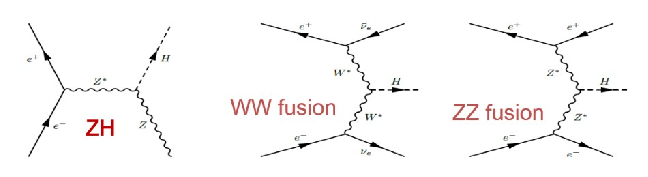
\includegraphics[width=0.75\textwidth]{FMD}
\caption[]{Feynman diagrams for Higgs boson production mechanisms at CEPC}
\label{fig:fmd}
\end{center}
\end{figure}


%\subsection{Measurement of width of Higgs boson}
%In nonrelative quantum dynamics, the eigenvalue of hamitonian of free particle is mass. For a unstable particle, 
%its probability of existing in whole space is a function of time, $e^{-\Gamma t}$. $\Gamma$ in which is width. the physical 
%meaning is width of the function of mass's probability inducing to half of the highest.
%
%As we all known, the width of a particle is equal to sum of width product branch ratio of each decay mode. Once the width 
%has been measured, compared to the total width, we can know if the decay modes of this particle are complete. 
%
%Because the mass of Higgs boson is 125$\gev$, three decay modes, which have strong Yukawa coupling, $H\rightarrow t\bar{t}$, 
%$H\rightarrow WW$ and $H\rightarrow ZZ$, have been abstained. It makes width narrow enough, about 4$\mev$. Because the mass 
%resolution of LHC is 3 order higher than width of Higgs boson, the measurement of width is not very well in LHC. But we can 
%measure width indirectly through measurement of the absolute branch ratio of Higgs boson in CEPC. 
%
%To measure the width, we introduce four independent observables firstly:
%\begin{eqnarray}
%Y_1 = \sigma_{ZH} = F_1\cdot g_Z^2,
%\end{eqnarray}
%\begin{eqnarray}
%Y_2 = \sigma_{ZH} \cdot Br(H \rightarrow b\bar{b}) = F_2 \cdot \frac{g_Z^2g_b^2}{\Gamma_H},
%\end{eqnarray}
%\begin{eqnarray}
%Y_3 = \sigma_{\nu\bar{\nu}H} \cdot Br(H \rightarrow b\bar{b}) = F_3 \cdot \frac{g_W^2g_b^2}{\Gamma_H},
%\end{eqnarray}
%\begin{eqnarray}
%Y_4 = \sigma_{ZH} \cdot Br(H \rightarrow b\bar{b}) = F_4 \cdot \frac{g_W^2g_W^2}{\Gamma_H},
%\end{eqnarray}
%where $g_Z$, $g_W$ and $g_b$ are couplings of Higgs to $ZZ$,$ WW$ and $b\bar{b}$ respectively;
%$F_1$, $F_2$, $F_3$ and $F_4$ are factors which can be calculated unambiguously. With these
%four observable the couplings and total width can be obtained as follows:
%\begin{itemize}
%\item From the measurement of $Y_1$ we can get the coupling $g_Z = \sqrt{\frac{Y_1}{F_1}}$,
%\item From the ratio $Y_2/Y_3$ we can get the coupling ratio $g_Z/g_W = \sqrt{\frac{Y_2F_3}{Y_3F_2}}$,
%\item With $g_Z$ and $g_Z/g_W$, we can get $g_W = \sqrt{\frac{Y_1Y_3F_2}{Y_2F_1F_3}}$,
%\item With $g_Z$ and $g_W$ known, from the measurement of $Y_4$ we can get the Higgs
%total width $\Gamma_H = \frac{Y_1^2Y_3F_2F_4}{Y_2Y_4F_1^2F_3}$.
%\end{itemize}
%In this note, we can get a important input for measurement, the branch ratio of $H\rightarrow WW^*$. And the other results 
%would be given by other collabration or CEPC.

\subsection{Classification of signal final states}
A full simulation study of the measurement of Br($H\rightarrow WW^*$) at the CEPC is highly motivated. Firstly, 
the SM Higgs boson branching ratio to $WW^*$ is 22\%, which renders is the most important channel 
to study the $HWW$ coupling at the CEPC. Moreover, the Br($H\rightarrow WW^*$) measurement is also 
a key ingredient for the determination of the Higgs boson width. Last but not least, the $W$ bosons decay into various physics 
objects (leptons, missing energy and momentum, taus and jets), providing an excellent benchmark to evaluate detector 
performance. The current status of the CEPC full simulation studies for the measurement of branch ratio BR($H\rightarrow WW^*$)
is reported in this note. 

For the studies discussed here,  the $H\rightarrow WW^*$ decays are classified into 50 different channels according to
the number of electrons, muons, tau-leptons, neutrinos and jets in the final state.
Assuming one million Higgs bosons, the expected yield for $H\rightarrow WW^*$ events in these final states 
is presented in Table~\ref{tab:list}. 
These final states are further classified into four categories depending on the number of jets in the event. As shown in
Table~\ref{tab:list} there can be, zero, two, four or six jet events.
\begin{table}[H]
  \begin{center}
    \begin{tabular}{|c|c|c|c|c|c|}
      \hline \hline
      \backslashbox{$W$ boson decay}{$Z$ boson decay}      & $ee$ & $\mu\mu$ & $\tau\tau$ & $\nu\nu$ & $qq$ \\
      \hline
      $WW^*\rightarrow e\nu e\nu$	&	\multicolumn{1}{>{\columncolor{mygray}}c|}{88}	
	  								&	\multicolumn{1}{>{\columncolor{mygray}}c|}{88}	
									&	\multicolumn{1}{>{\columncolor{mygray}}c|}{88} 	
	  								&	\multicolumn{1}{>{\columncolor{mygray}}c|}{603} 	
									&	\multicolumn{1}{>{\columncolor{green}}c|}{1836}\\
	  \hline                                                                
      $WW^*\rightarrow \mu\nu\mu\nu$&	\multicolumn{1}{>{\columncolor{mygray}}c|}{87}	
	  								&	\multicolumn{1}{>{\columncolor{mygray}}c|}{87}	
									&	\multicolumn{1}{>{\columncolor{mygray}}c|}{87}	
									&	\multicolumn{1}{>{\columncolor{mygray}}c|}{593}		
									&	\multicolumn{1}{>{\columncolor{green}}c|}{1808}\\
      \hline                                                                
      $WW^*\rightarrow e\nu\mu\nu$	&	\multicolumn{1}{>{\columncolor{mygray}}c|}{175}	
	  								&	\multicolumn{1}{>{\columncolor{mygray}}c|}{175}	
									&	\multicolumn{1}{>{\columncolor{mygray}}c|}{175}	
									&	\multicolumn{1}{>{\columncolor{mygray}}c|}{1206}	
									&	\multicolumn{1}{>{\columncolor{green}}c|}{3644}\\
      \hline                                                                
	  $WW^*\rightarrow e\nu\tau\nu$	&	\multicolumn{1}{>{\columncolor{mygray}}c|}{187}	
	  								&	\multicolumn{1}{>{\columncolor{mygray}}c|}{187}	
									&	\multicolumn{1}{>{\columncolor{mygray}}c|}{188}	
									&	\multicolumn{1}{>{\columncolor{mygray}}c|}{1281}	
									&	\multicolumn{1}{>{\columncolor{green}}c|}{3901}\\
	  \hline                                                                
	  $WW^*\rightarrow \mu\nu\tau\nu$&	\multicolumn{1}{>{\columncolor{mygray}}c|}{186}	
	  								&	\multicolumn{1}{>{\columncolor{mygray}}c|}{186}	
									&	\multicolumn{1}{>{\columncolor{mygray}}c|}{186}	
									&	\multicolumn{1}{>{\columncolor{mygray}}c|}{1271}	
									&	\multicolumn{1}{>{\columncolor{green}}c|}{3872}\\
	  \hline                                                                
	  $WW^*\rightarrow \tau\nu\tau\nu$&	\multicolumn{1}{>{\columncolor{mygray}}c|}{99}	
	  								&	\multicolumn{1}{>{\columncolor{mygray}}c|}{99}	
									&	\multicolumn{1}{>{\columncolor{mygray}}c|}{99}	
									&	\multicolumn{1}{>{\columncolor{mygray}}c|}{681}		
									&	\multicolumn{1}{>{\columncolor{green}}c|}{2072}\\
      \hline                                                                
      $WW^*\rightarrow e\nu qq$		&	\multicolumn{1}{>{\columncolor{green}}c|}{1111}
	  								&	\multicolumn{1}{>{\columncolor{green}}c|}{1112}
									&	\multicolumn{1}{>{\columncolor{green}}c|}{1114}
									&	\multicolumn{1}{>{\columncolor{green}}c|}{7589}	
									&	\multicolumn{1}{>{\columncolor{magenta}}c|}{23112}\\
      \hline                                                                
      $WW^*\rightarrow \mu\nu qq$ 	&	\multicolumn{1}{>{\columncolor{green}}c|}{1103}
	  								&	\multicolumn{1}{>{\columncolor{green}}c|}{1104}
									&	\multicolumn{1}{>{\columncolor{green}}c|}{1105}
									&	\multicolumn{1}{>{\columncolor{green}}c|}{7530}	
									&	\multicolumn{1}{>{\columncolor{magenta}}c|}{22939}\\
      \hline                                                                
	  $WW^*\rightarrow \tau\nu qq$	&	\multicolumn{1}{>{\columncolor{green}}c|}{1181}
	  								&	\multicolumn{1}{>{\columncolor{green}}c|}{1182}
									&	\multicolumn{1}{>{\columncolor{green}}c|}{1183}
									&	\multicolumn{1}{>{\columncolor{green}}c|}{8066}	
									&	\multicolumn{1}{>{\columncolor{magenta}}c|}{24558}\\
	  \hline                                                                
	  $WW^*\rightarrow qqqq$ 		&	\multicolumn{1}{>{\columncolor{magenta}}c|}{3498}
	  								&	\multicolumn{1}{>{\columncolor{magenta}}c|}{3502}
									&	\multicolumn{1}{>{\columncolor{magenta}}c|}{3506}
									&	\multicolumn{1}{>{\columncolor{magenta}}c|}{23884}	
									&	\multicolumn{1}{>{\columncolor{red}}c|}{72735}\\
      \hline \hline
    \end{tabular}
   \caption[Monte Carlo purities in the single lepton sample]{Signal events of the  
     $Z\rightarrow X, H\rightarrow WW^*, WW^* \rightarrow X$ processes.
     The different colours denote different jet categories: zero-jet category (gray), two-jet
     category (green), four-jet category (magenta), and six-jet category (red).}
  \label{tab:list}
 \end{center}
\end{table}

In this note, a representative analysis of each jet category is reported in detail. For the zero-jet category, 
$e^+e^-\rightarrow ZH, Z\rightarrow \mu^+\mu^-, H\rightarrow WW^*, WW^*\rightarrow e\nu\mu\nu$ decay chain has been considered. 
For categories with jets the following decay chains have been studied:
$e^+e^-\rightarrow ZH, Z\rightarrow e^+e^-,  H\rightarrow WW^*, WW^*\rightarrow \mu\nu qq$ (two-jet category)  
and $e^+e^-\rightarrow ZH, Z\rightarrow \nu\nu,  H\rightarrow WW^*, WW^*\rightarrow qqqq$ (four-jet category).
The six-jet category is more complicated and will be the topic of a future analysis.


%This manuscript is organized as following. The second section described the detector geometry implemented in the full simulation. 
%The MC sample,simulation and reconstruction tools are introduced, and to reduce the consumption of computing power, general 
%event filters has been applied to the CEPC Higgs analsis, which is reported in section 3. Section 4 is devided into three parts, 
%each corresponding to one representative analysis of different $H\rightarrow WW^*$ decay mode. In section 5, the results of all 
%individual analysis are combined, leading to an accuracy of Br($H\rightarrow WW^*$) measurement. Conclusion and outlooks are 
%summarized in Section 6.

%\section{The CEPC detector}
%The CEPC conceptual detector design is based on ILC detector designs, as illustrated in Figure~\ref{fig:acepcdetector}. 
%\begin{figure}[H]
%	\centering
%	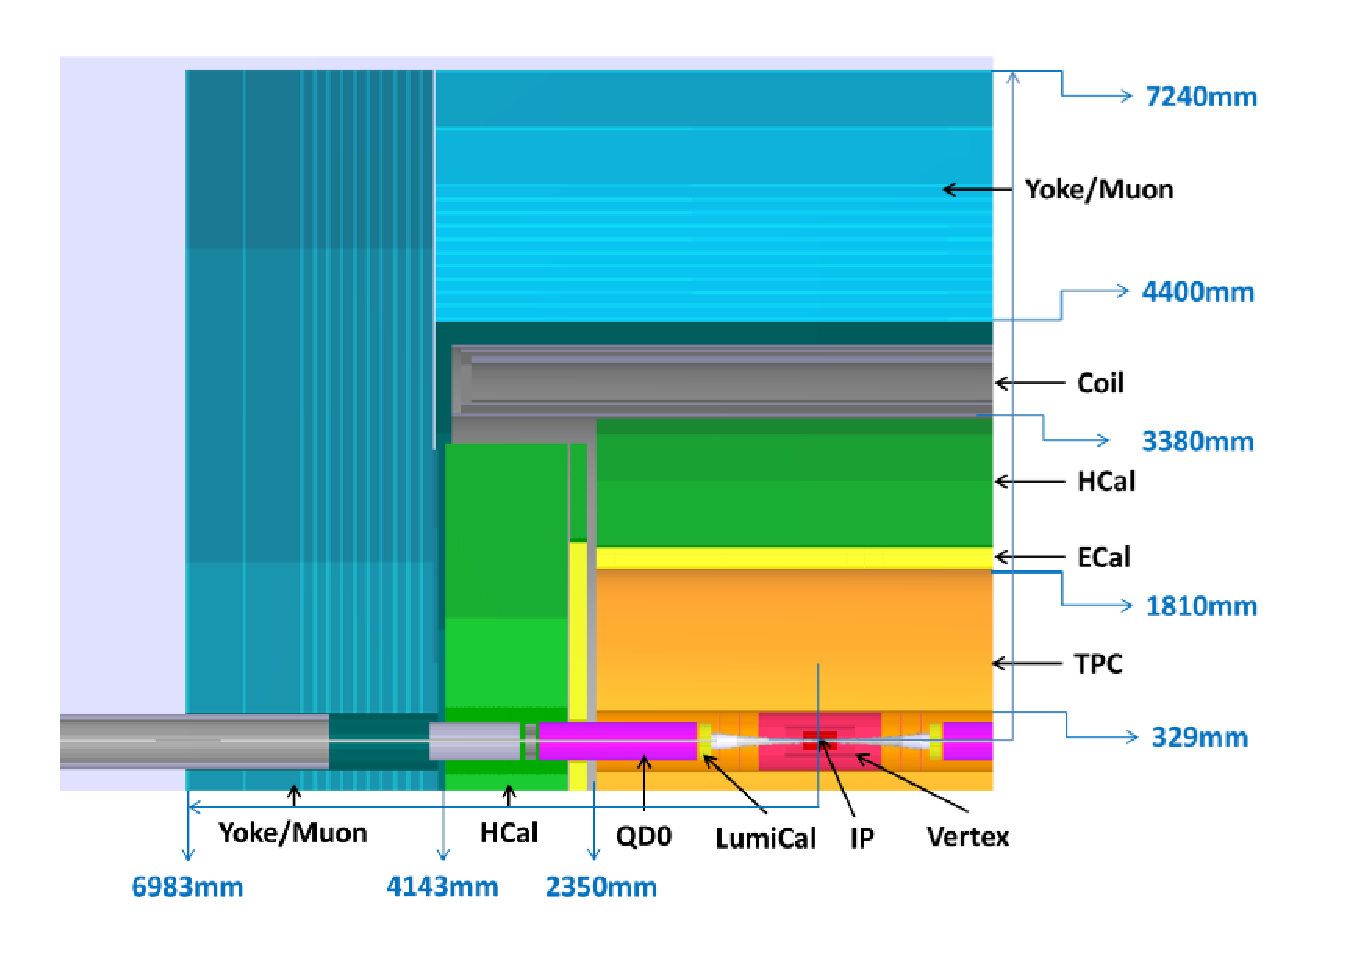
\includegraphics[width=0.7\textwidth]{cepcdetector}
%	\caption[]{Overview of the CEPC detector}
%	\label{fig:acepcdetector}
%\end{figure}
%The CEPC detectoe consists of the following sub-detectors:
%\begin{itemize}
%	\item A vertex detector(VTX) construted with high resolution pixel sensors. 
%		The vertex detector is placed very close to the intreaction point, withan inner radius of 16mm. 
%		This vertex detector ensures excellent tagging capability of $b\text{-}/c\text{-}$quark jets and $\tau\text{-}$leptons.
%	\item A silicon tracker composed of Silicon Inner Tracker(SIT), Forward Tracking Disks(FTDs), 
%		Silicon External Tracker(SET) and End-cap Tracking Disks(ETDs). The VTX and SIT provide 
%		excellent spatial measurement near the IP, crucial for vertex reconstruction and jet flavor tagging. 
%		The SET and ETD, on the other handm provide excellent spatial resolution with the maximal possible 
%		track arm length, therefore improving the track momentum resolution of charged particles. 
%		The FTDs significantly increases the geometric acceptance of the tracking system with coverage of $|\cos\theta| < 0.99$. 
%	\item A Time Projection Chanber(TPC) with a half-length of 2.35m and an outer radius of 1.8m.
%		The TPC provides a large number of spatial points ($\sim$200 hits per track) and spatial resolution 
%		in $r\phi$ plane better than 100$\mu$m. It has excellent pattern recognition and track reconstruction 
%		efficiency(better than 97\% for tracks with $p_T > 1\gev$).
%	\item A calorimetry system consists of Electromagnetic Calorimeter(ECal) and Hadron Calorimeter(HCal) 
%		with very fine granularity. The system plays an essential role in the Particle-Flow Algorithm(PFA), 
%		allowing excellent separation of showers from different particles, and provides jet energy resolution of 3 - 4\%.
%	\item A superconducting solenoid of 3.5T surrounds the calorimetry system. The return yoke is placed outside the solensid. 
%	\item A muon detector with tracking layers installed in the return yoke. 
%\end{itemize}

\section{MC samples}
\subsection{Simulation and analysis tools}
This analysis is performed using simulated data that correspond to an integrated luminosity of 5000fb$^{-1}$ at $\sqrt s =250\gev$.
The cross section and No. of events for the various processes relevant for this energy is shown in Figure~\ref{fig:csf} and Table~\ref{tab:vocandnoe}. 
For all signal samples a Higgs boson mass of $m_H = 125\gev$ is assumed. 
Background events are generated by Whizard 1.95~\cite{Kilian:2007gr} and include initial state radiation (ISR). 
The detector model, cepc\_v1~\cite{CEPC-SPPCStudyGroup:2015csa}, is simulated by {\tt Geant4}~\cite{Agostinelli:2002hh}. 
Object reconstruction is done using the particle-flow algorithm, {\tt Arbor}~\cite{Ruan:2014paa}.
Charged particle identification is performed by LICH~\cite{Yu:2017mpx}, 
which is a TMVA-based~\cite{Therhaag:2009dp} software package optimized for a high granularity calorimeter~\cite{Brient:2002gh}. 
The $ee$-$k_T$ clustering algorithm is used for jet clustering and the performance of the $b$-tagging algorithm is given by 
LCFIPlus package~\cite{Suehara:2015ura}.

\begin{figure}[H]
	\begin{center}
		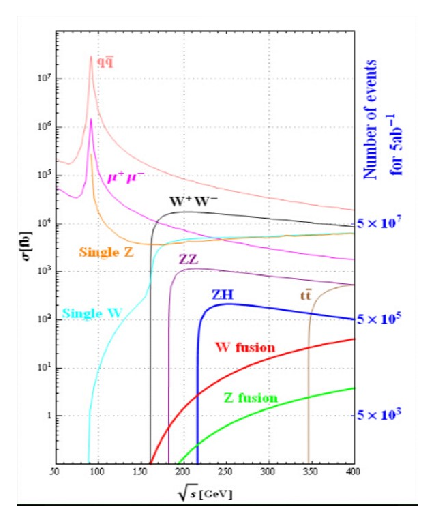
\includegraphics[width=0.35\textwidth]{CSF}
	\end{center}
	\caption[]{The distribution of cross section of the Standard Model when center mass of system is near 250~\gev.}
		\label{fig:csf}
\end{figure}
\begin{table}[H]
	\begin{center}
	\begin{tabular}{ccc}
		\hline\hline
		Process	&	Cross Section in fb	&	Number of Events in 5000fb$^{-1}$	\\
		\hline
		\multicolumn{3}{ c }{\textbf{\large Higgs production}}	\\
		\hline
		$ZH$	&	212					&	$1.06\times 10^6$	\\
		$\nu\bar{\nu}H$&	6.27		&	$3.36\times 10^4$	\\
		$e^+e^-H$	&	0.63			&	$3.15\times 10^3$	\\
		\hline
		total	&	219					&	$1.10\times 10^6$	\\
		\hline\hline
		\\
		\multicolumn{3}{ c }{\textbf{\large Standard Model Background}}	\\
		\hline
		qq		&	50216				&	$2.5\times 10^8$	\\
		$\mu\mu$&	4405				&	$2.2\times 10^7$	\\
		$WW$	&	15484				&	$7.7\times 10^7$	\\
		$ZZ$	&	1033				&	$5.2\times 10^6$	\\
		$eeZ$(single $Z$)	&	4734	&	$2.4\times 10^7$	\\
		$e\nu W$(single $W$)&	5144	&	$2.6\times 10^7$	\\
		\hline
		total	&	801016				&	$3.54\times 10^8$	\\
		\hline\hline
	\end{tabular}
	\end{center}
	\caption[]{The specific value of cross section and No. of events of the signal processes and the main Standard Model when center mass of system is 250~\gev.}
	\label{tab:vocandnoe}
\end{table}

The SM backgrounds included in this search are classified in two-fermion and four-fermion final states.
Two fermion backgrounds include  Bhabha scattering and the production of $\mu^+\mu^-$, $\tau^+\tau^-$, $\nu\bar{\nu}$ and $q\bar{q}$ pairs.
Four fermion background consist of rest of the SM backgrounds.
This includes also $ZH$ production in which the Higgs boson decays to channels other than $WW$.

\subsection{Pre-selection}
The total background to the branching ratio measurement amounts to more than 30 million events according to Table~\ref{tab:vocandnoe}.
Many of those events, however, have completely different topologies compared to signal, and therefore
the decision to reject them can be made at an early stage, even before the simulation.

The events are categorized to four classes: $llH(l=e,\mu)$, $\tau\tau H$, 
$\nu\nu H$ and $qqH$. Subsequently,  a loose selection is performed on the objects
before they are passed to the full detector simulation, which will be referred to in the
following as pre-selection. The pre-selection is such that it is fully efficient for
signal events.

\subsubsection{Pre-selection of $e^+e^- \rightarrow ZH, Z\rightarrow l^+l^-(l=e,\mu), H\rightarrow X$ decay}
Compared to the SM background, the most distinguishing feature of 
$Z\rightarrow l^+l^-(l=e,\mu), H\rightarrow X$ decays is the invariant mass 
and the recoil mass of $Z$ boson. For the pre-selection, {\color{blue}all the leptons with same flavor would be looped, 
and two of them which combined invariant mass is nearest to mass of $Z$ boson are selected.} 
And subsequently a window in the di-lepton invariant mass and in the recoil mass
is required with numerical values shown in Table~\ref{tab:llhprecut}.
%And the plots of invariant mass and recoil mass are in Appendix~\ref{}.
\begin{figure}[H]
	\centering
	\subfigure[]{
		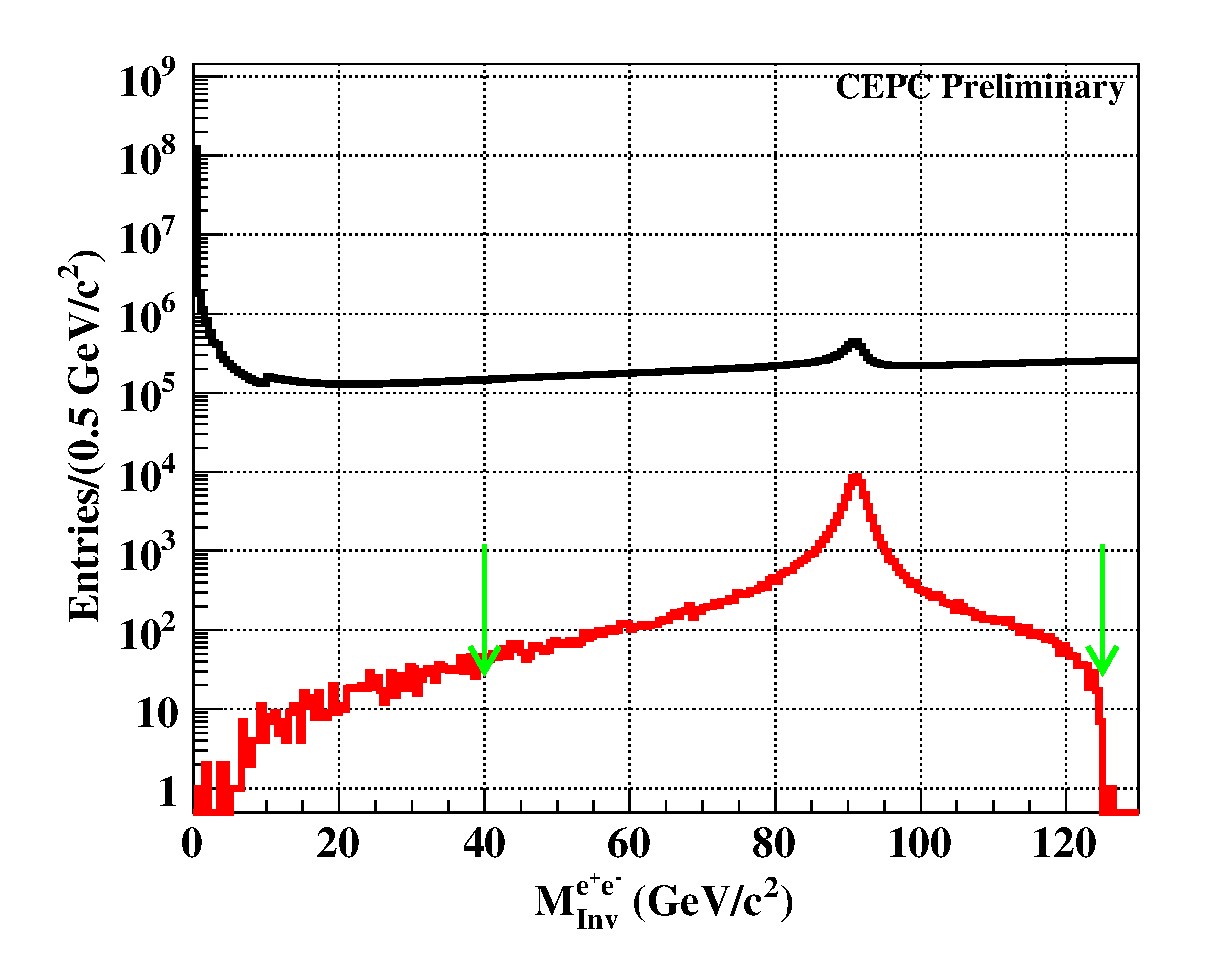
\includegraphics[width=0.35\textwidth]{filterfig/mcfig/e1e1H/eeHInvMass}
		\label{fig:eeHfilterInvMass}
	}
	\subfigure[]{
		 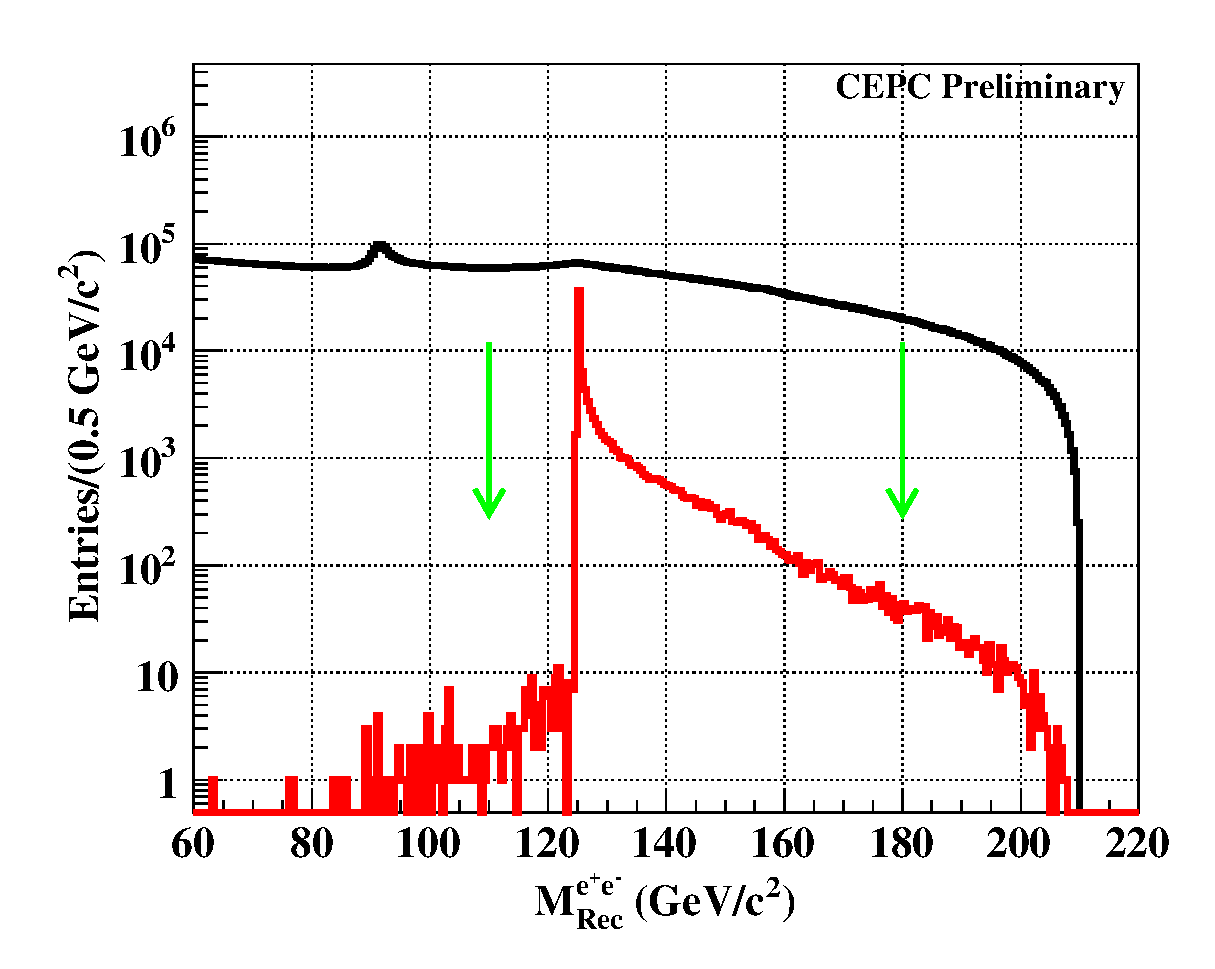
\includegraphics[width=0.35\textwidth]{filterfig/mcfig/e1e1H/eeHRecMass}
		 \label{fig:eeHfilterRecMass}
	}
	\subfigure[]{
		\includegraphics[width=0.35\textwidth]{filterfig/mcfig/e2e2H/uuHInvMass}
		\label{fig:uuHfilterInvMass}
	}
	\subfigure[]{
		 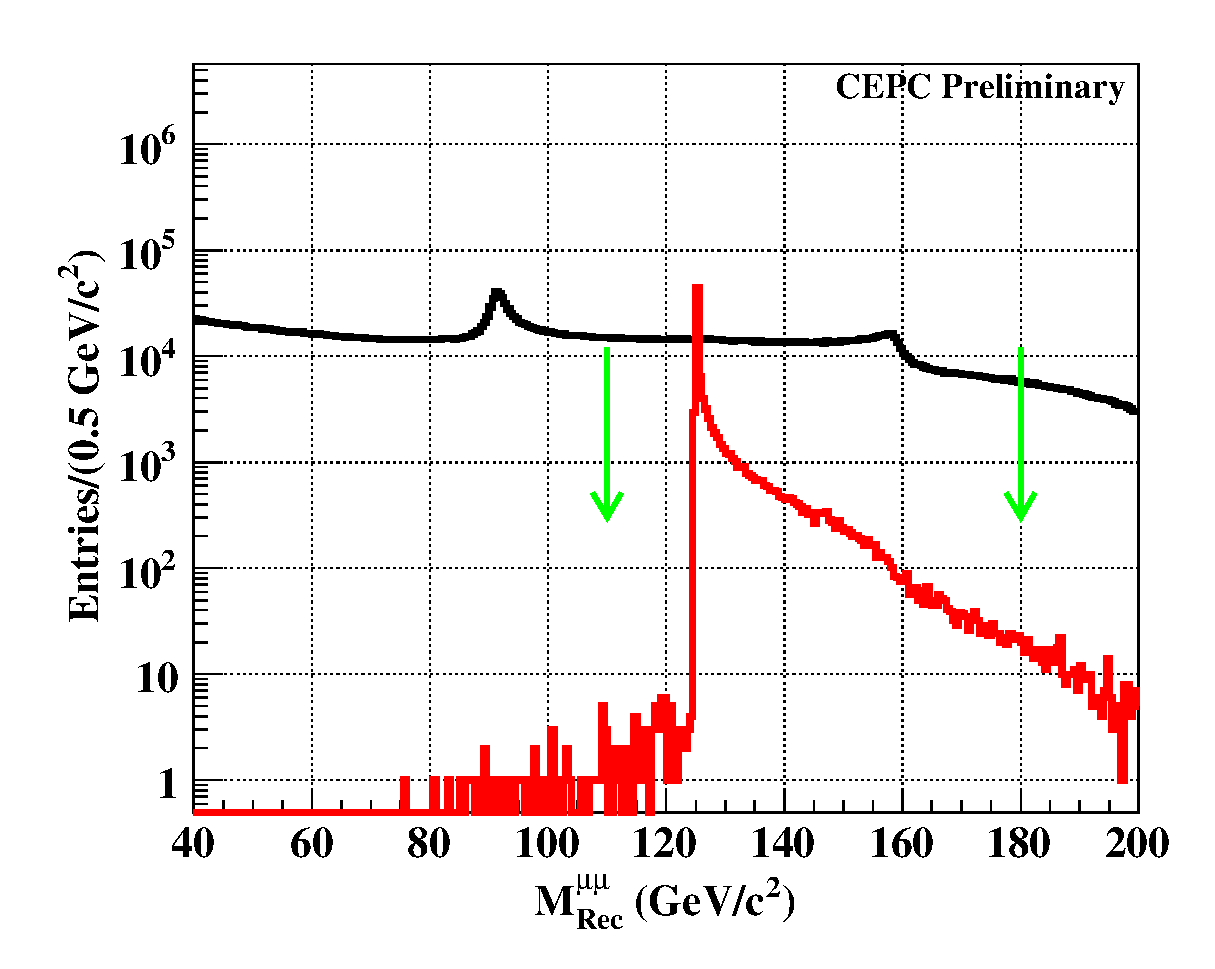
\includegraphics[width=0.35\textwidth]{filterfig/mcfig/e2e2H/uuHRecMass}
		 \label{fig:uuHfilterRecMass}
	}
	\caption[]{The distribution of invariant mass and recoil mass of the best candidate of $Z$ boson. 
	Red line is the distribution of Higgs signal. Black line is the distribution of the Standard Model background.
	TOP: These two plots are the mass distribution of $Z\rightarrow e^+e^-, H\rightarrow X$ decay.
	Bottom: The left is invariant mass distribution and right is recoil mass distribution of $Z\rightarrow \mu^+\mu^-, H\rightarrow X$ decay.}
	\label{fig:llHfilter}
\end{figure}
	
	After applied the pre-selection in MC level and full simulated, the same variable of pre-selection should 
	be valid, as shown in Figure~\ref{fig:llHfiltered}, and the cut windows shown in Table~\ref{tab:llhprecut}.
\begin{figure}[H]
	\centering
	\subfigure[]{
		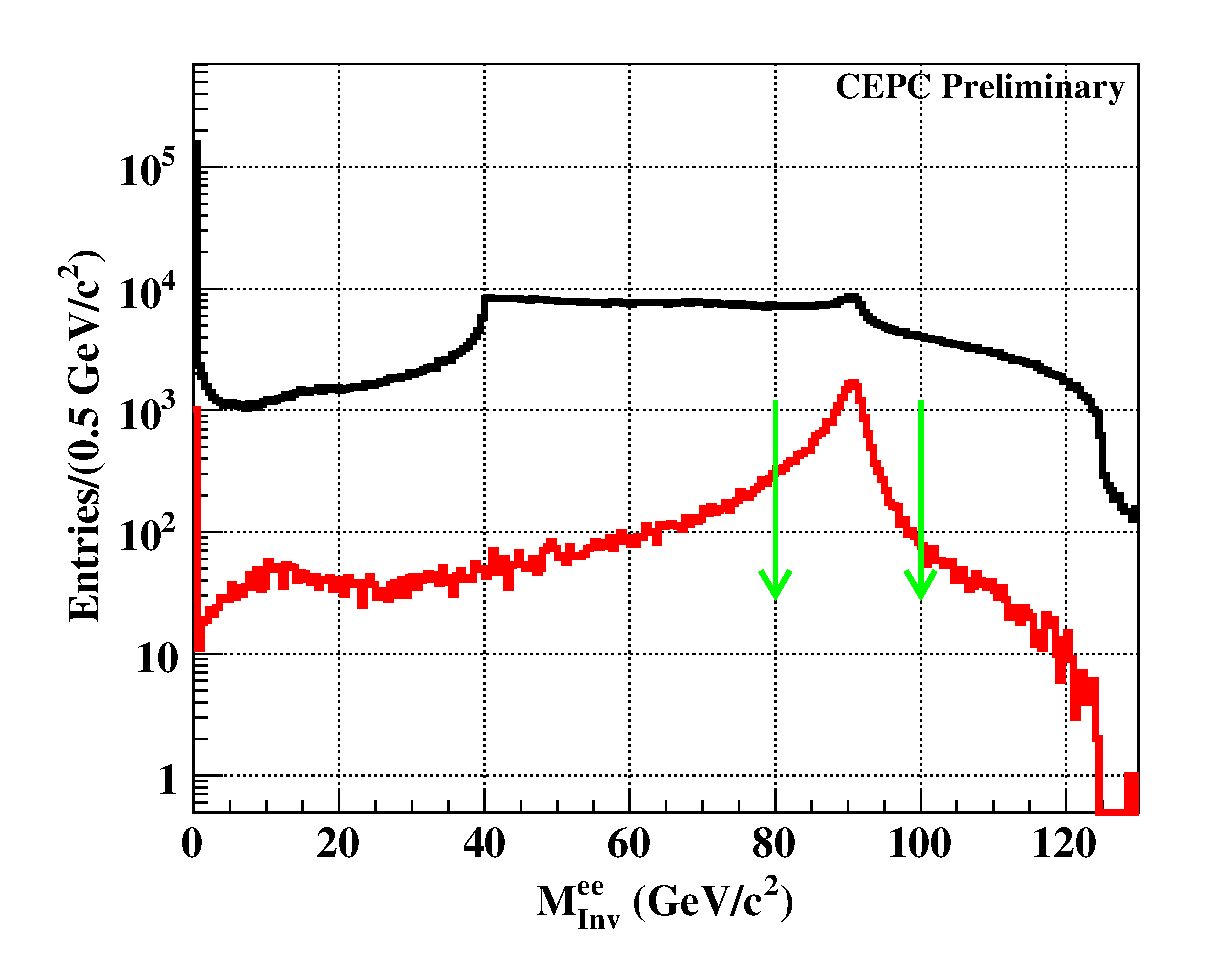
\includegraphics[width=0.35\textwidth]{filterfig/fullsim/e1e1H/InvMass}
		\label{fig:eeHfilteredInvMass}
	}
	\subfigure[]{
		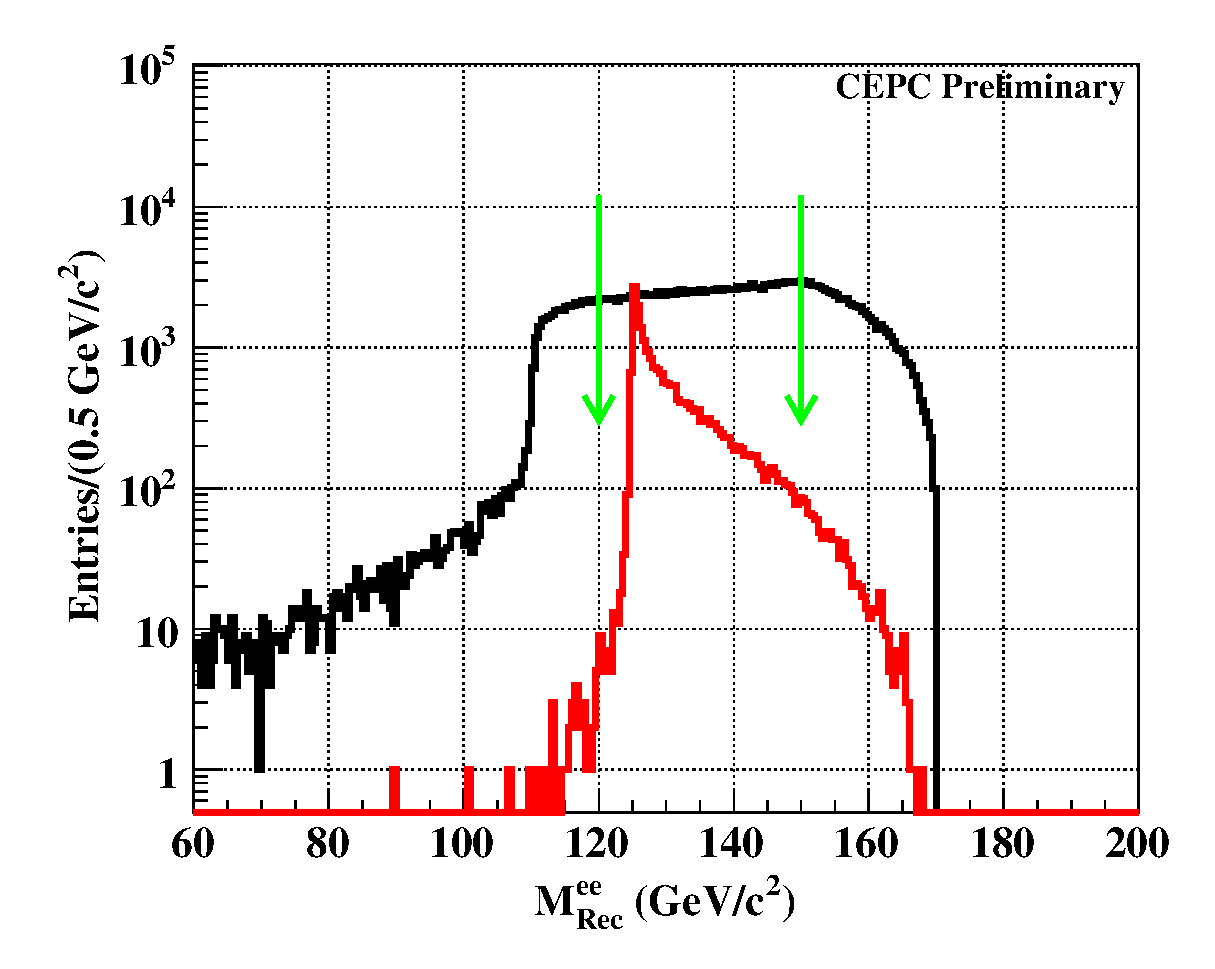
\includegraphics[width=0.35\textwidth]{filterfig/fullsim/e1e1H/RecMass}
		\label{fig:eeHfilteredRecMass}
	}
	\subfigure[]{
		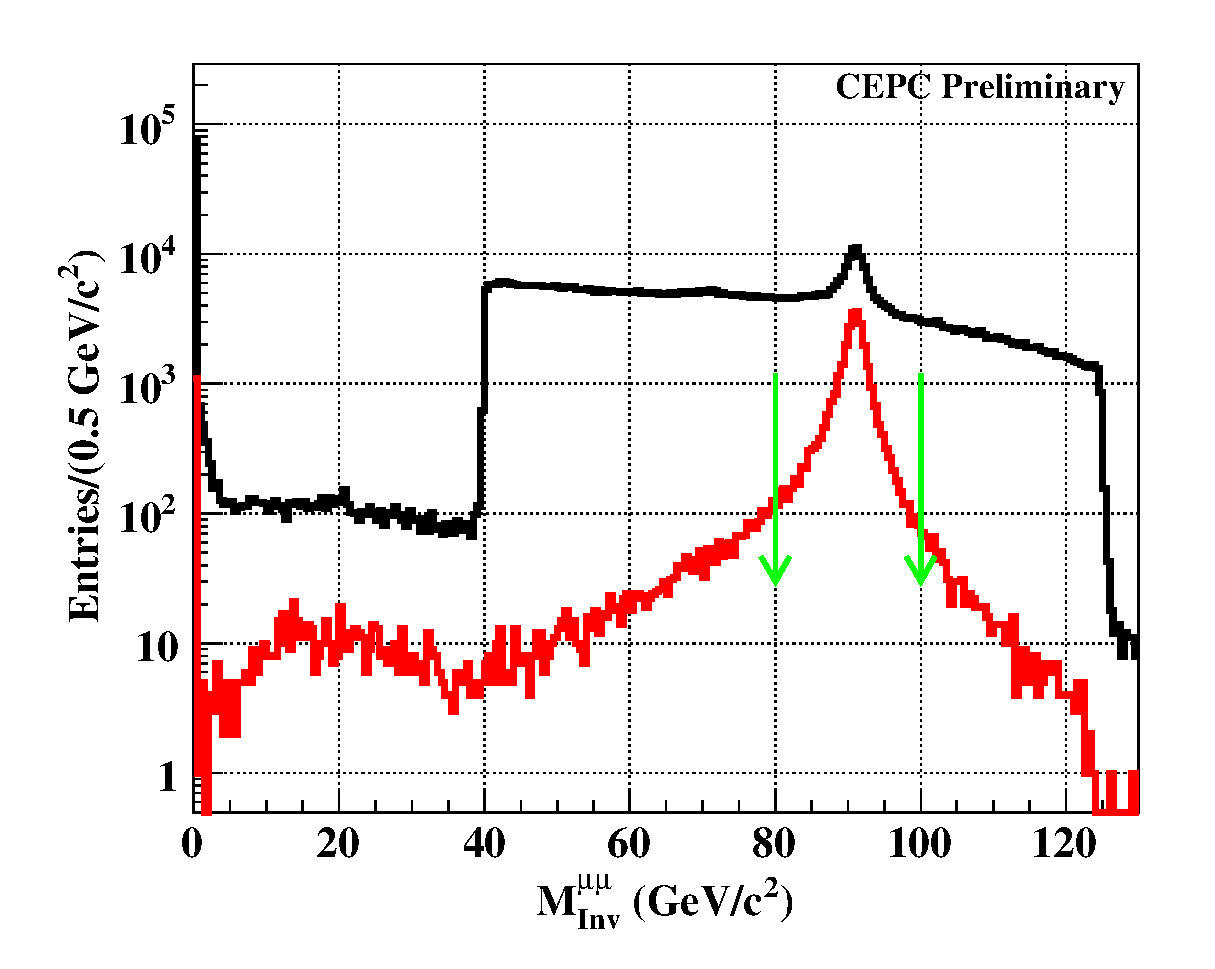
\includegraphics[width=0.35\textwidth]{filterfig/fullsim/e2e2H/InvMass}
		\label{fig:uuHfilteredInvMass}
	}
	\subfigure[]{
		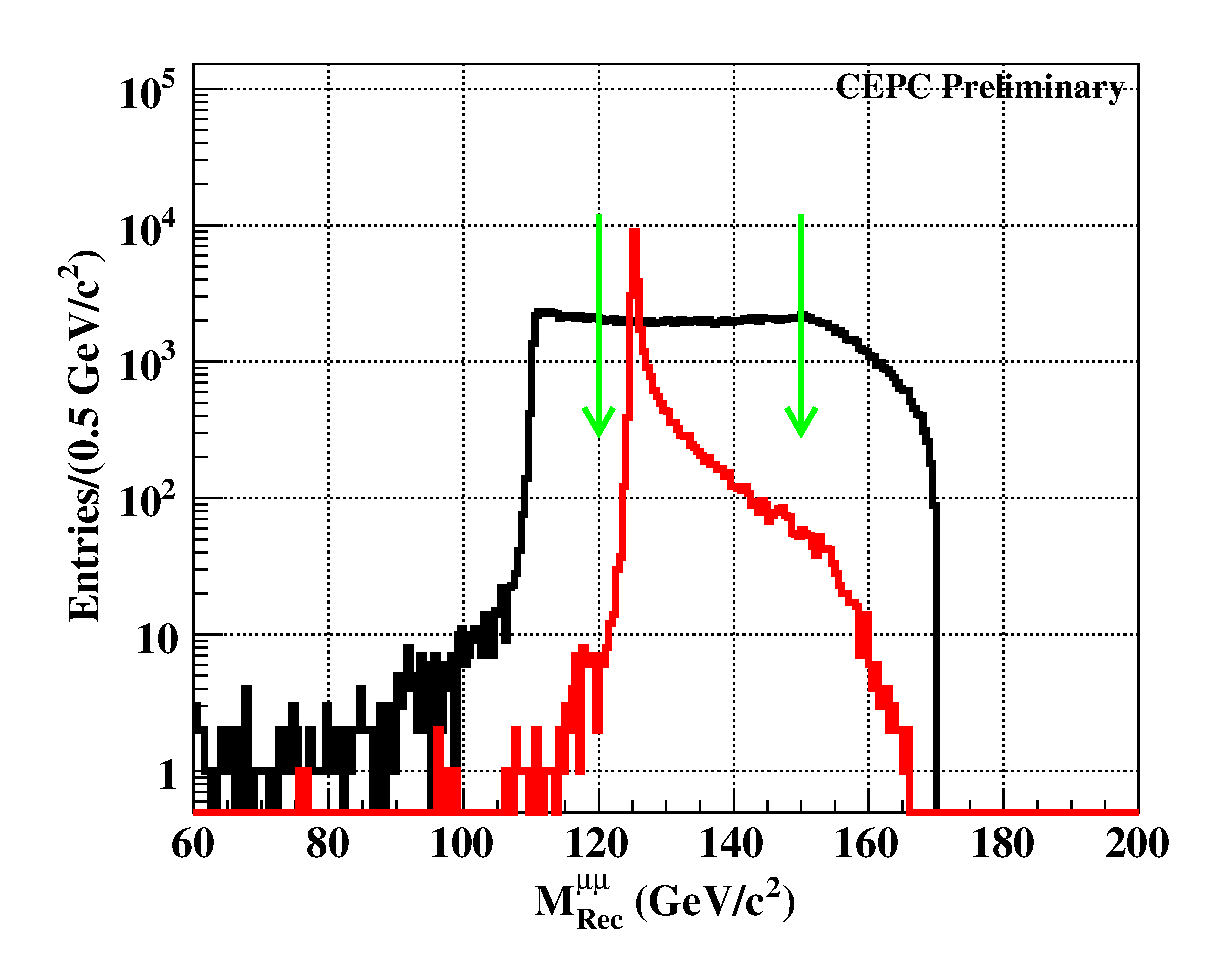
\includegraphics[width=0.35\textwidth]{filterfig/fullsim/e2e2H/RecMass}
		\label{fig:uuHfilteredRecMass}
	}
	\caption[]{The distribution of invariant mass and recoil mass of the best candidate of $Z$ boson in full simulation. 
	Red line is the distribution of Higgs signal. Black line is the distribution of the Standard Model background.
	TOP: These two plots are the mass distribution of $Z\rightarrow e^+e^-, H\rightarrow X$ decay.
	Bottom: The left is invariant mass distribution and right is recoil mass distribution of $Z\rightarrow \mu^+\mu^-, H\rightarrow X$ decay.}
	\label{fig:llHfiltered}
\end{figure}

\begin{table}[H]
\newcommand{\tabincell}[2]{\begin{tabular}{@{}#1@{}}#2\end{tabular}}
 \begin{center}
  \begin{tabular}{|c|c|c|}
  \hline \hline
  Process of signal				&		$eeH$ process						&				$\mu\mu H$ process\\
  \hline
  \multirow{2}{*}{conditions of pre-selection} 	&	$40\gev/c^2 < M_{Inv}^{ee} < 130\gev/c^2$&$40\gev/c^2 < M_{Inv}^{\mu\mu} < 130\gev/c^2$	\\
  											&	$110\gev/c^2 < M_{Rec}^{ee} < 180\gev/c^2$		&$110\gev/c^2 < M_{Rec}^{\mu\mu} < 180\gev/c^2$\\
  \hline
  \multirow{2}{*}{conditions of validation}	&	$80\gev/c^2 < M_{Inv}^{ee} < 100\gev/c^2$&$80\gev/c^2 < M_{Inv}^{\mu\mu} < 100\gev/c^2$	\\
  											&	$120\gev/c^2 < M_{Rec}^{ee} < 150\gev/c^2$		&$120\gev/c^2 < M_{Rec}^{\mu\mu} < 150\gev/c^2$\\
  \hline \hline
  \end{tabular}
  \caption[]{Conditions of pre-selection in MC and validation in full simulation. Considered the resolution of detector, 
  the conditions of validation should be more strict.}
  \label{tab:llhprecut}
 \end{center}
\end{table}
This pre-selection is highly efficient for signal: more than 95\% of signal event are retained. At the same time
more than 99\% of the background events are rejected. 

\subsubsection{Pre-selection of $e^+e^- \rightarrow ZH, Z\rightarrow \nu\bar{\nu}, H\rightarrow X$ decay.}
The pre-selection of $\nu\nu H$ channel is less trivial to define compared to
$eeH$ and $\mu\mu H$ decay chains. Due to the $Z\to\nu\nu$ decay, it is 
possible to use the missing mas of the event to discriminate between signal 
and background. In addition to the missing mass, the total mass
and the total transverse momentum are used, as well as {\color{blue}the polar angle of each final state particle
$|cos\theta| < 0.99$ is contained}.
\begin{figure}[H]
	\centering
	\subfigure[]{
		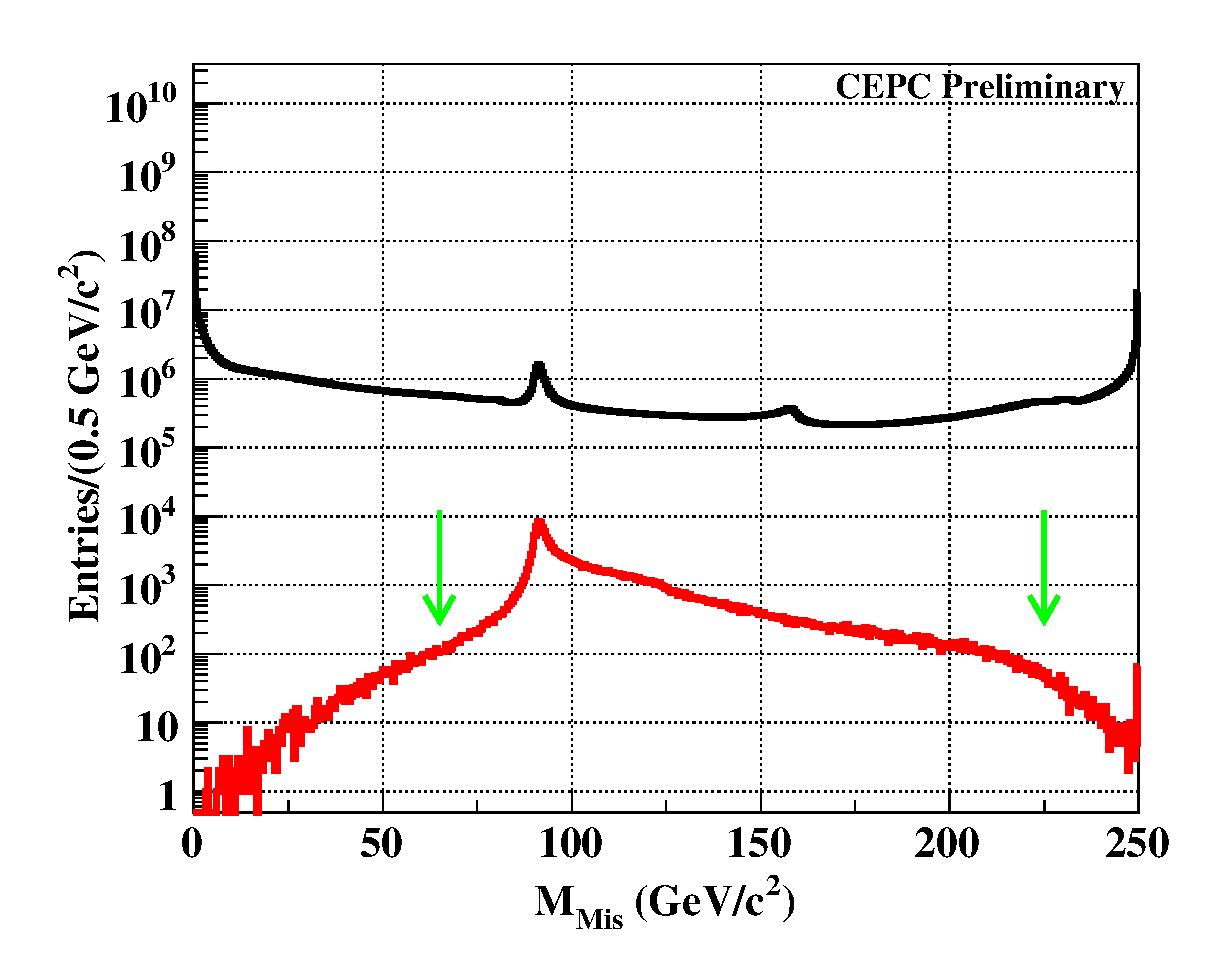
\includegraphics[width=0.35\textwidth]{filterfig/mcfig/nnH/MisMass}
		\label{fig:nnHfilterMisMass}
	}
	\subfigure[]{
		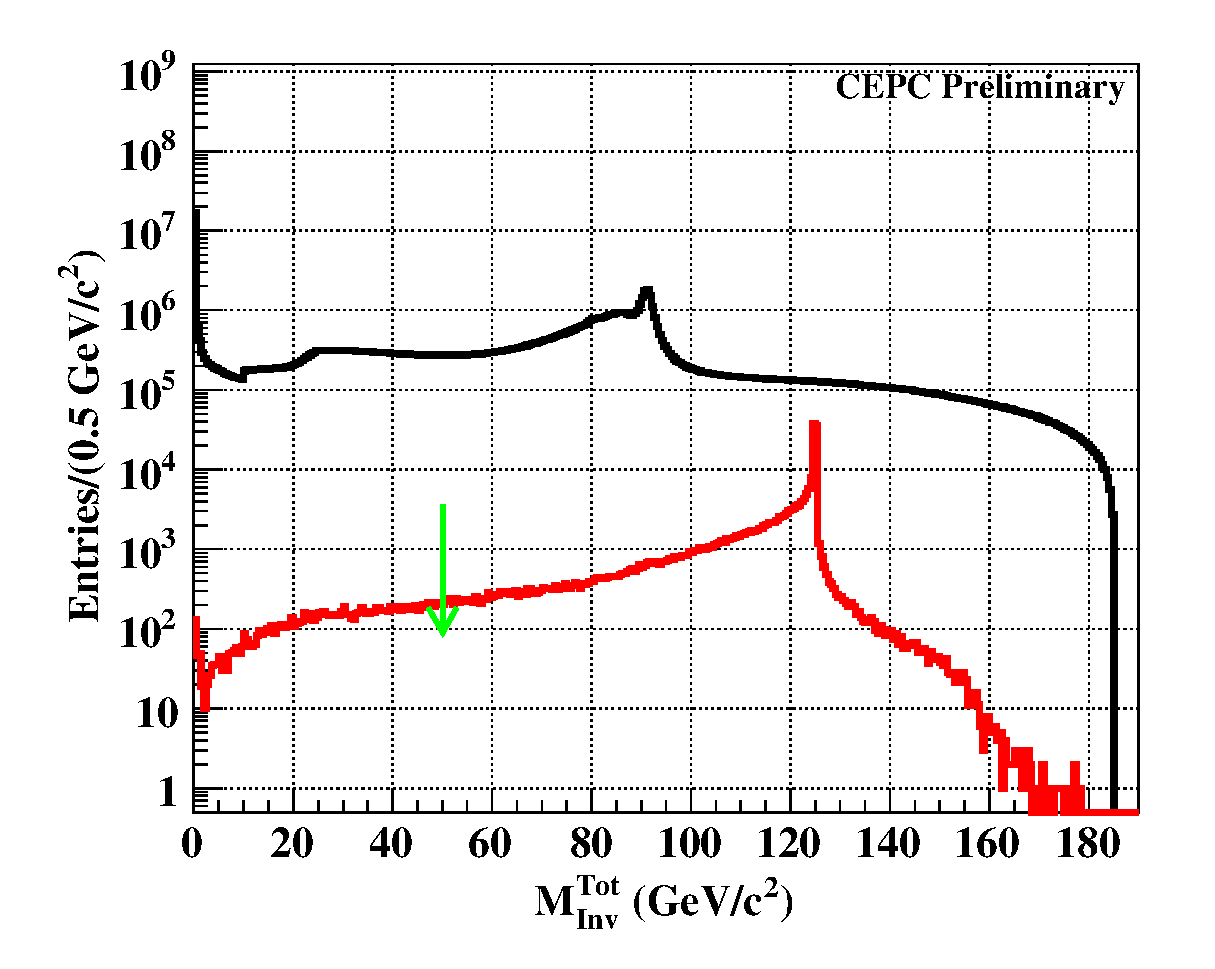
\includegraphics[width=0.35\textwidth]{filterfig/mcfig/nnH/TotalM}
		\label{fig:nnHfilterTotalM}
	}
	\subfigure[]{
		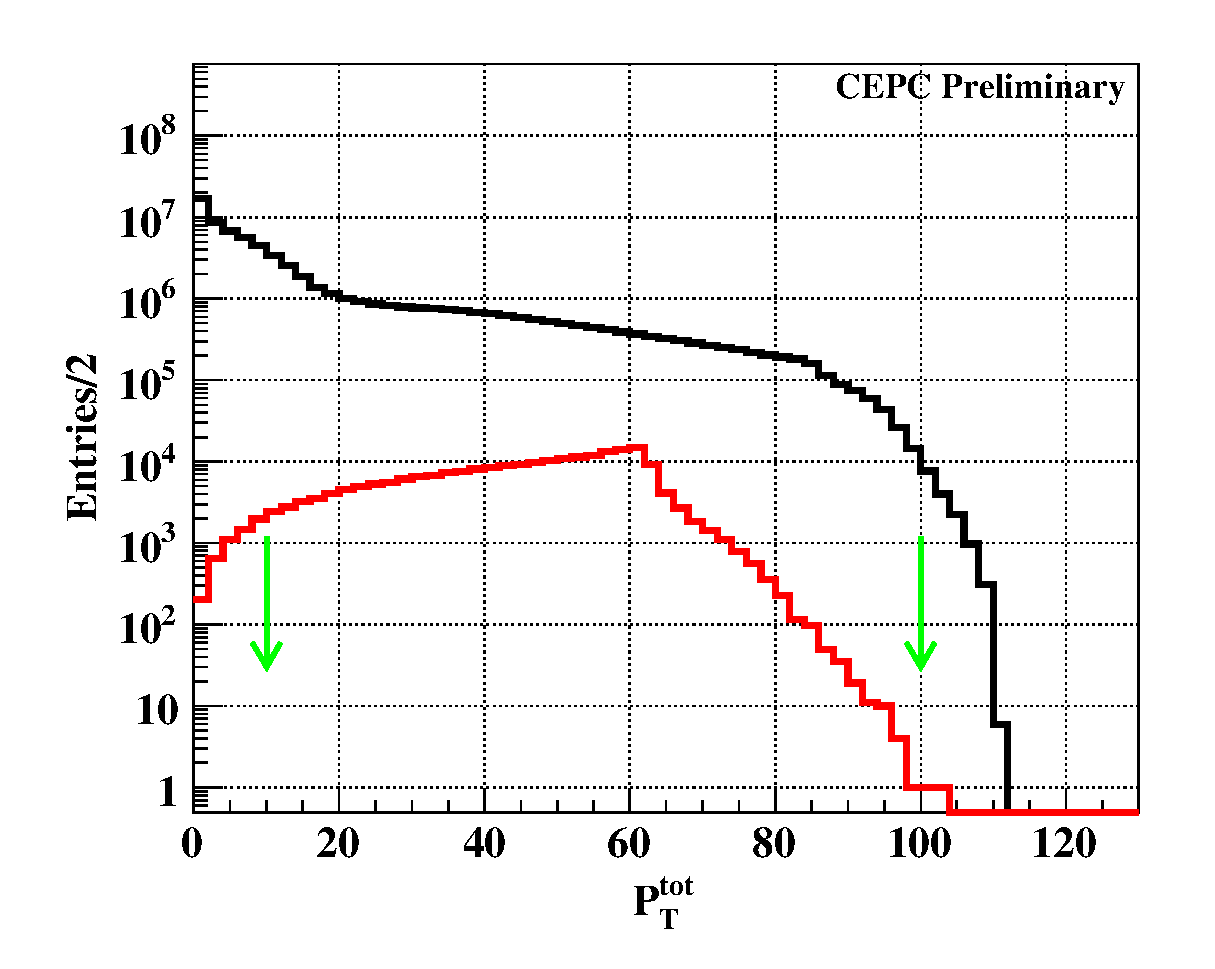
\includegraphics[width=0.35\textwidth]{filterfig/mcfig/nnH/TotalPt}
		\label{fig:nnHfilterTotalPt}
	}
	\caption[]{The distribution of missing mass, total mass and total transverse momentum in MC truth. 
	Red line is the distribution of Higgs signal. Black line is the distribution of the Standard Model background.
	Top: The left is missing mass of event. The right is total mass of event.
	Bottom: It is the distribution of total transverse momentum of event.}
	\label{fig:nnHfilter}
\end{figure}

As same as the $Z\to ll$ decay channel, after applied the pre-selection in MC, the same variable should be valid 
in full simualtion.
\begin{figure}[H]
	\centering
	\subfigure[]{
		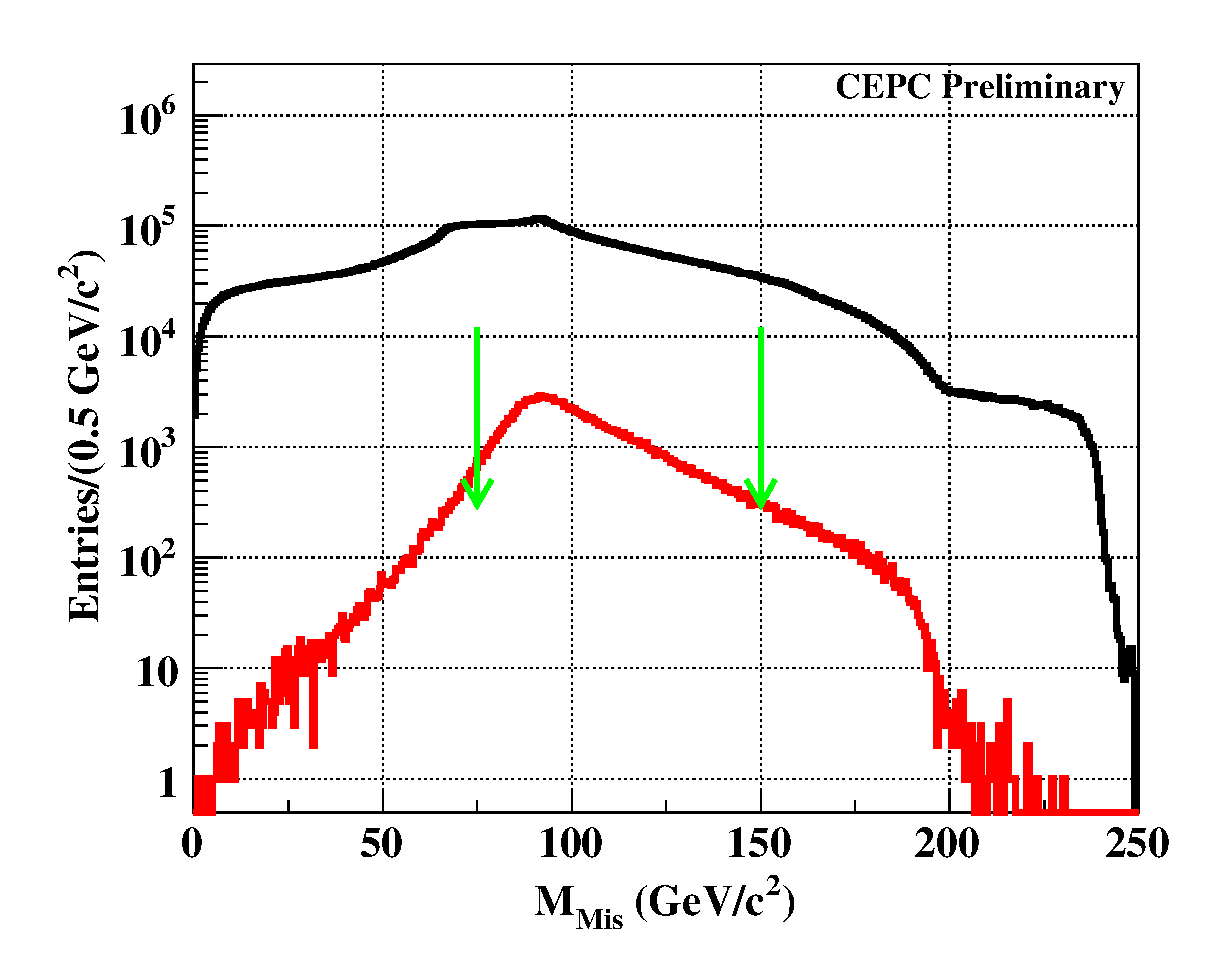
\includegraphics[width=0.35\textwidth]{filterfig/fullsim/nnH/MisMass}
		\label{fig:nnHfilteredMisMass}
	}
	\subfigure[]{
		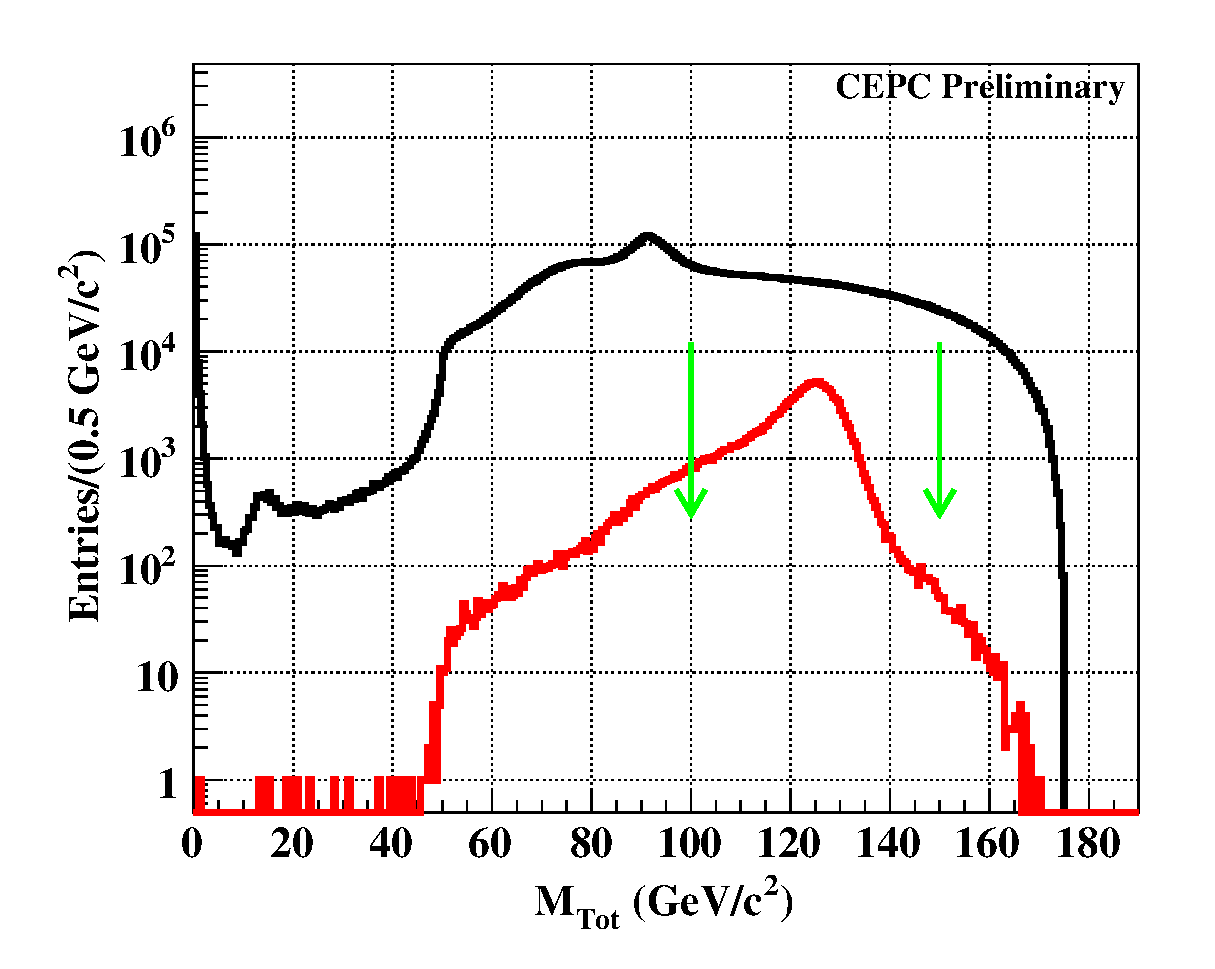
\includegraphics[width=0.35\textwidth]{filterfig/fullsim/nnH/TotalMass}
		\label{fig:nnHfilteredTotalM}
	}
	\subfigure[]{
		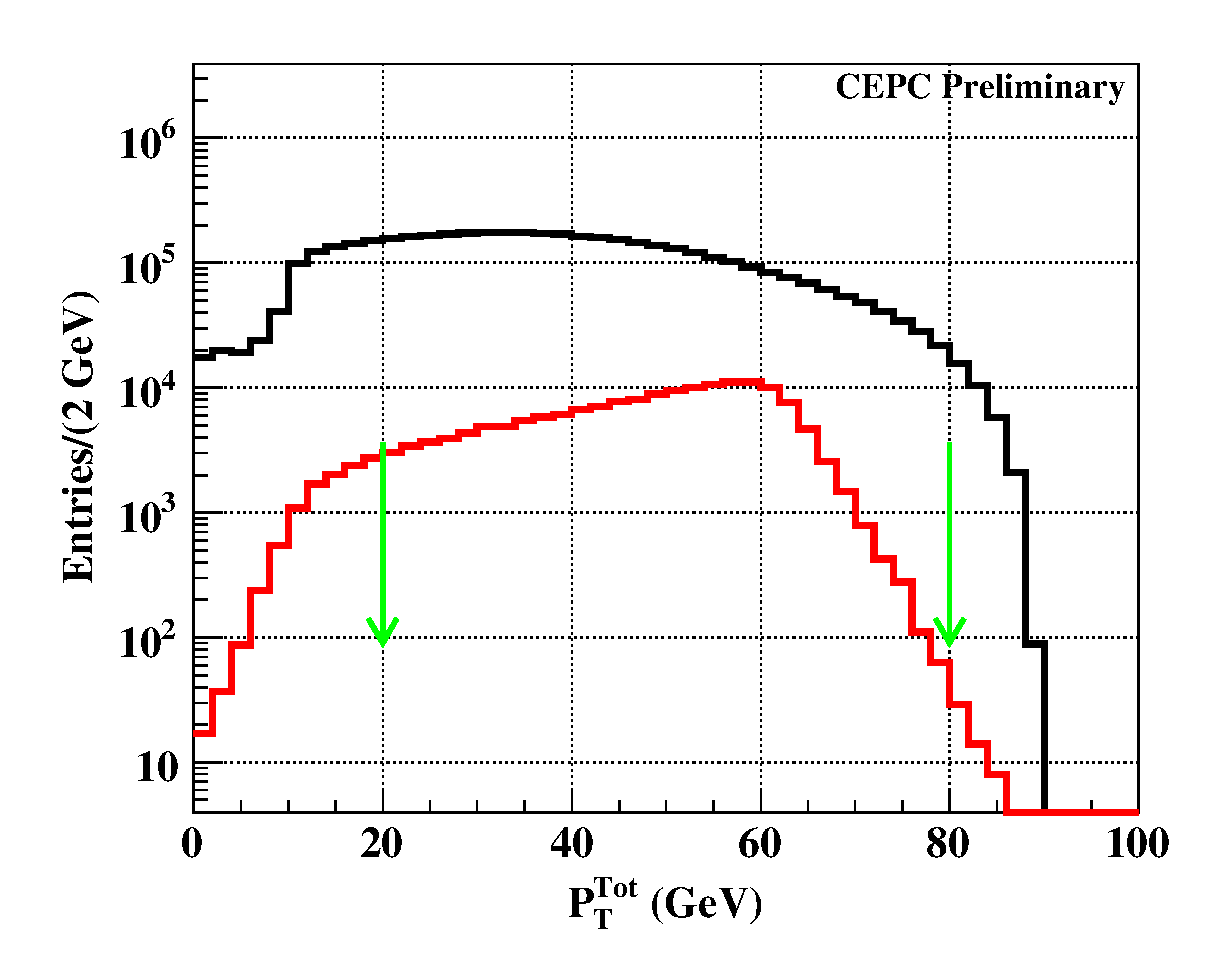
\includegraphics[width=0.35\textwidth]{filterfig/fullsim/nnH/TotalPt}
		\label{fig:nnHfilteredTotalPt}
	}
	\caption[]{The distribution of missing mass, total mass and total transverse momentum in full simulation. 
	Red line is the distribution of Higgs signal. Black line is the distribution of the Standard Model background.
	Top: The left is missing mass of event. The right is total mass of event.
	Bottom: It is the distribution of total transverse momentum of event.}
	\label{fig:nnHfiltered}
\end{figure}
\begin{table}[H]
  \begin{center}
  \begin{tabular}{|c|c|}
  \hline \hline
  Process of signal								&				$\nu\nu H$\\
  \hline
  \multirow{3}{*}{conditions of pre-selection}	&	$65\gev/c^2 < M_{Mis} < 225\gev/c^2$	\\
  												&	$M_{Tot} > 50\gev/c^2$\\
												&	$10\gev/c < p_{T} < 100\gev/c$	\\
  \hline
  \multirow{3}{*}{conditions of validation}		&	$75\gev/c^2 < M_{Mis} < 150\gev/c^2$	\\
  												&	$100\gev/c^2 < M_{Tot} < 150\gev/c^2$	\\
												&	$20\gev/c < p_{T} < 80\gev/c$	\\
  \hline \hline
  \end{tabular}
  \caption[]{Conditions of pre-selection in MC and validation in full simulation of $\nu\nu H$ process}
 \end{center}
  \label{tab:nnhprecut}
\end{table}
The distributions of signal and background events are similar, as shown in
Figure~\ref{fig:nnHfilter}. The pre-selection conditions are defined in
Table~\ref{tab:nnhprecut} and take into account this feature.

The distribution of the same variables after reconstruction is shown in
Figure~\ref{fig:nnHfiltered}.
{\color{blue} Considering the resolution of detector, the conditions of pre-selection should be valided more strict in full simulation.}

%\subsection{Reconstruction software !!!!!!!!!!!!!!!!!!!!!!!!!!!}
%Arbor is a reconstruction software for CEPC. 
%In Table~\ref{tab:RecEffLep}, we show the reconstruction efficiency of leptons by Arbor. The reconstruction efficiency of electron is near 
%90\%, and of the muon is near 98\%.
%\begin{table}[H]
%  \begin{center}
%  	\begin{tabular}{|c|c|c|c|c|c|}
%      \hline \hline
%	  $Z$ boson decay & $W$ boson decay & Excepted	&	Yield & Observable	&	Efficiency	\\ 
%      \hline
%	  \multirow{5}{*}{$\mu^+\mu^-$}		& $e\nu e\nu$		&  89	&   88	&  76	&	86\%\\
%	  									& $\mu\nu\mu\nu$	&  87	&   89	&  80	&	90\% \\
%	  									& $e\nu\mu\nu$		&  176	&	174 &  157	&	90\% \\
%	  									& $e\nu q\bar{q}$	&  1117	&  1105	& 1042	&	94.3\%\\
%	  									& $\mu\nu q\bar{q}$	&  1106	&  1110	& 1056	&	95.1\%\\
%	  \hline
%	  \multirow{5}{*}{$e^+e^-$}			& $e\nu e\nu$ 	 	&  95	&	91	&  62	&	68\%\\
%	  									& $\mu\nu\mu\nu$ 	&  94	&	82	&  63	&	77\% \\
%	  									& $e\nu\mu\nu$	 	&  188	&	178 &  132	&	74\% \\
%	  									& $e\nu q\bar{q}$	&  1195	&	1182& 1041	&	80.1\% \\
%	  									& $\mu\nu q\bar{q}$	& 1184	&	1221& 1194	&	80.0\% \\
%      \hline \hline
%    \end{tabular}
%   \caption[Monte Carlo purities in the single lepton sample]{Resonstruction efficiency of leptons in each decay channels. Excepted is the 
%   number of the theoretical events. Yield is the number of real generation events. Observable is the number of true events 
%   after leptons' and jets' number selection. The efficiency is observable over yield.}
%  \label{tab:RecEffLep}
% \end{center}
%\end{table}

\section{Measurement of $Br(H\rightarrow WW^*)$}
After the pre-selection is defined, the sensitivity estimation of
the measurement of the branching ratio can proceed. Due to the large number 
of possible decay chains only a subset of them will be considered in the
following, as discussed earlier.


\subsection{Analysis of $e^+e^-\rightarrow ZH, Z\rightarrow\mu^+\mu^-, H\rightarrow WW^*, WW^*\rightarrow e\nu\mu\nu$ decay}
\label{sec:uuevuv}
\subsubsection{Event selection}
The $e^+e^-\rightarrow ZH, Z\rightarrow\mu^+\mu^-, H\rightarrow WW^*, WW^*\rightarrow e\nu\mu\nu$ channel is selected because it contains
two different flavour leptons in the final state, which can be used very effectively to supress the backgrounds.

The requirement of exactly three muons and one electron {\color{blue}and less than three remain neutral particles} in the event has been
shown in Ref.~\cite{Mo:2015mza} to allow only small backgrounds
due to $ZZ\rightarrow \mu^+\mu^-\tau^+\tau^-$ and $ZZ\rightarrow 4\tau$ decays.
Hence, the main background is due to other Higgs boson decays, such as $H\to\tau\tau$.

{\color{blue} To cut down these Higgs background and $ZZ$ events background, the combined invariant mass of $e$ and $\mu$
within $10~\gev/c^2$ and $ 65~\gev/c^2$, and missing mass of event less than $65~\gev/c^2$, are applied.}

The SM background is further reduced by the expected excellent performance
of the CEPC vertex detector (VTX), which is planned to be 
constructed with high resolution pixel sensors near the interaction point(IP) 
resulting in resolution better than $4\mu m$.
{\color{blue}By requiring $\sqrt{(\frac{D_{0}}{sigD_{0}})^2+(\frac{Z_{0}}{sigZ_{0}})^2} < 5$ for $e$ and $\mu$ decayed from $W$ boson, 
$D_0$ and $sigD_0$ showed the derivation in X-Y plane, $Z_0$ and $sigZ_0$ showed the derivation in Z direction,
it is efficient to discriminate the background events of $\tau$ leptons or heavy flavour quarks.}

\begin{figure}[H]
\centering
	\subfigure[]{
		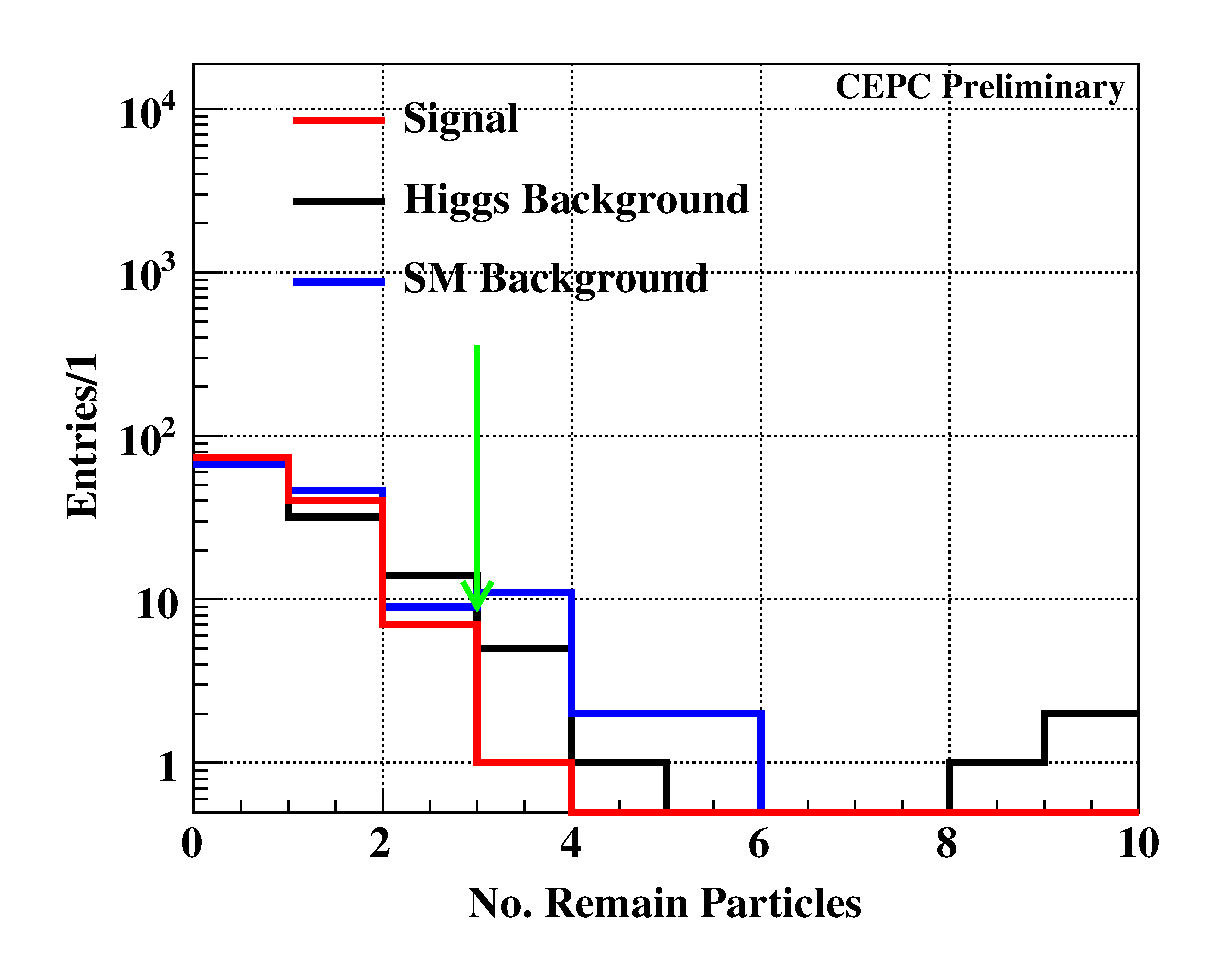
\includegraphics[width= 0.35\textwidth]{e2e2H/evuv/nRem}
		\label{fig:euRem}
	}
	\subfigure[]{
		\includegraphics[width= 0.35\textwidth]{e2e2H/evuv/llInvMass}
		\label{fig:eullInv}
	}
	\subfigure[]{
		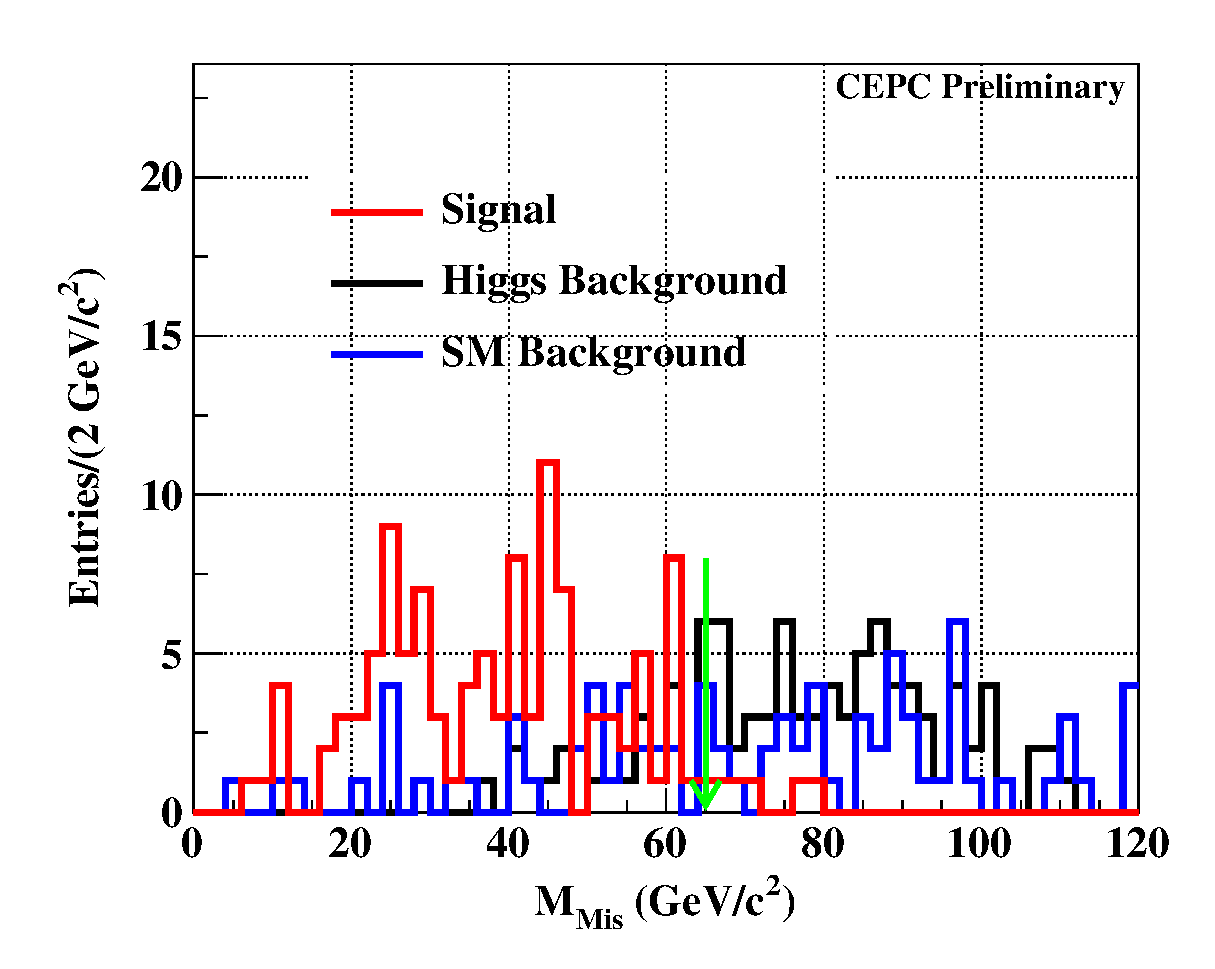
\includegraphics[width= 0.35\textwidth]{e2e2H/evuv/MisMass}
		\label{fig:euMisMass}
	}
	\subfigure[]{
		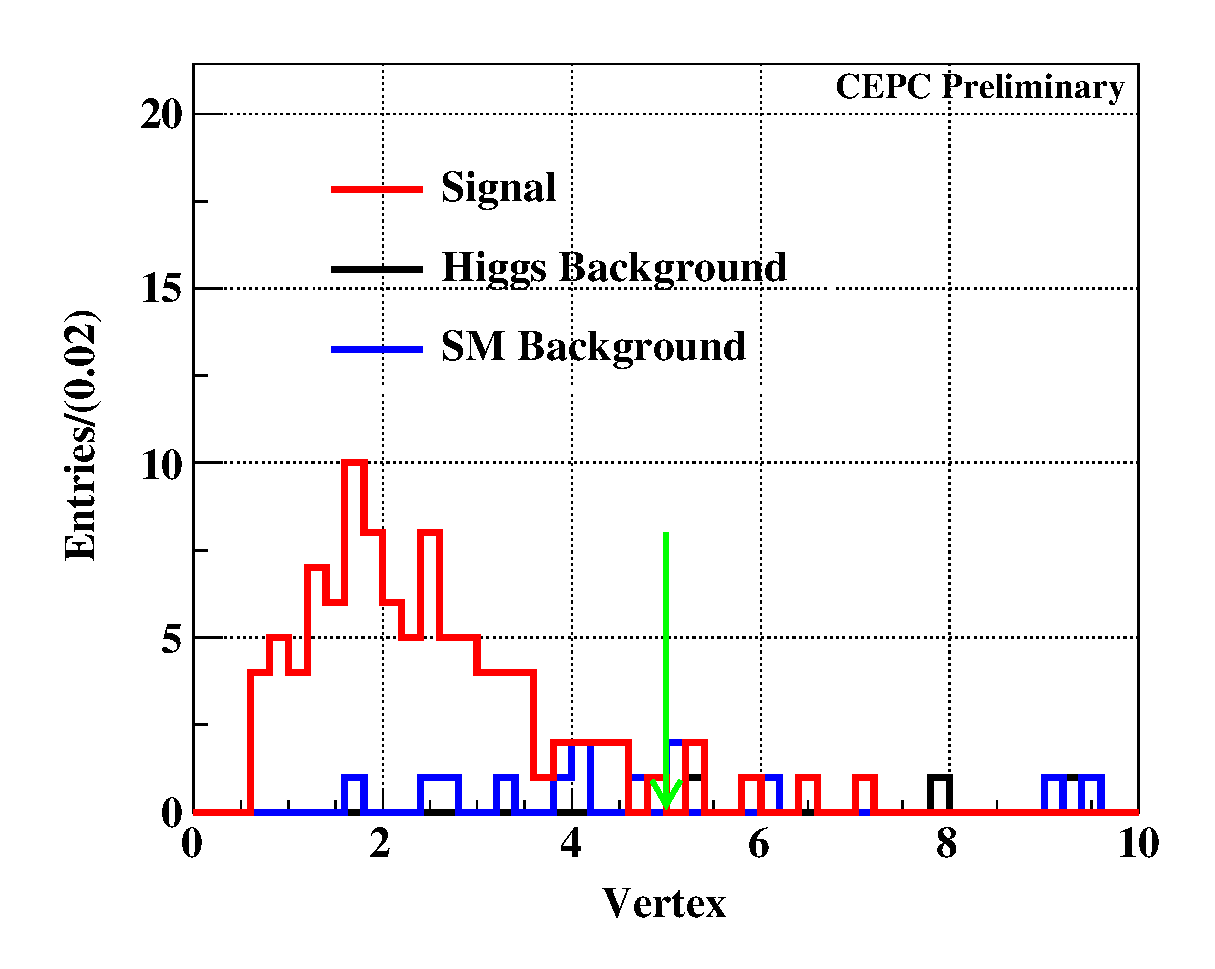
\includegraphics[width= 0.35\textwidth]{e2e2H/evuv/Vertex}
		\label{fig:euVertex}
	}
	\caption[]{
		\ref{fig:euRem} The No. remain particles of $e^+e^-\rightarrow ZH, Z\rightarrow\mu^+\mu^-, H\rightarrow WW^*,  
		WW^*\rightarrow e\nu\mu\nu$ decay. Except for four tracks, there are few photons, so we can veto semi-leptonic decay
		and hadronic decay of background.
		\ref{fig:eullInv} The distribution of combined invariant mass of electron and muon. 
		Since these two leptons decayed from different $W$ boson, the combined invariant mass of them 
		should be less than the mass of on-shell $W$ boson.
		\ref{fig:euMisMass} The distribution of missing mass of event. Since there are two neutrinos in this signal process 
		and much more neutrinos in background, four in $ZZ$ background and $H\to\tau\tau$ background, the missing mass should 
		be less than them.
		\ref{fig:euVertex} The distribution of Vertex of $e^+e^-\rightarrow ZH, Z\rightarrow\mu^+\mu^-, H\rightarrow WW^*, 
		WW^*\rightarrow e\nu\mu\nu$ decay. And there are two leptons totally from $W$ boson, so we plus the value of each lepton.
		And leptons from $\tau$ and $b$-jet would fly a long distance, so they would be rejected effectively.}
	\label{fig:euRemandVertex}
\end{figure}

The number of events passing each selection step is shown in Table~\ref{tab:emu}. The main background of this channel comes from
the  $e^+e^-\rightarrow  ZZ\rightarrow\tau^+\tau^-\mu^+\mu^- $ process, as shown in Table~\ref{tab:uueubkg}.
\begin{table}[H]
\begin{center}
\begin{tabular}{cccc}
\hline \hline
\multicolumn{1}{c}{Category}& \multicolumn{1}{c}{Signal}&\multicolumn{1}{c}{$ZH$ background}&\multicolumn{1}{c}{SM background}\\   
\hline
  Total                                                 &     172   & 34624 &700311\\
  Validation of pre-selection				            &     136   & 29263 & 117395\\
  $N_{ZPole}=2; N_{Isolep}=2; l_1 = e, l_2 = \mu$       &     122   &   145 &   150  \\
  $N_{Remain} < 3$                                      &     121   &   113 &   122   \\
  $10\gev < M_{Inv}^{e\mu} < 65\gev$                    &     116   &   101 &   87  \\
  $M_{Missing} < 65\gev/c^2$                      		&     110   &   26  &   36   \\
  $\sqrt{(\frac{D0}{sigD0})^2+(\frac{Z0}{sigZ0})^2} < 5$&     93    &   3   &   10   \\
  \hline \hline
  \end{tabular}
  \caption[Monte Carlo purities in the single lepton sample]{% Monte
	  The final event selection of $e^+e^-\rightarrow ZH, Z\rightarrow\mu^+\mu^-, H\rightarrow WW^*, WW^*\rightarrow e\nu\mu\nu$ decay.}
\label{tab:emu}
\end{center}
\end{table}
\begin{table}[H]
\begin{center}
\begin{tabular}{lrc}
\hline\hline
Decay Chain	& Final States 	&	Number of Events\\
\hline
$e^+e^-\rightarrow ZZ, ZZ\rightarrow\tau^+\tau^-\mu^+\mu^- $	& $\mu^+, \mu^-, \tau^+, \tau^-$			&10	\\
\hline\hline
\end{tabular}
\caption{Summery of total background with the same final states of signal event}
\label{tab:uueubkg}
\end{center}
\end{table}

\subsubsection{Statistical result}
The distribution of the recoil mass of the $\mu^+\mu^-$ system after 
the selection is shown in Figure~\ref{fig:uuhevuvrecfit}.
\begin{figure}[H]
\centering
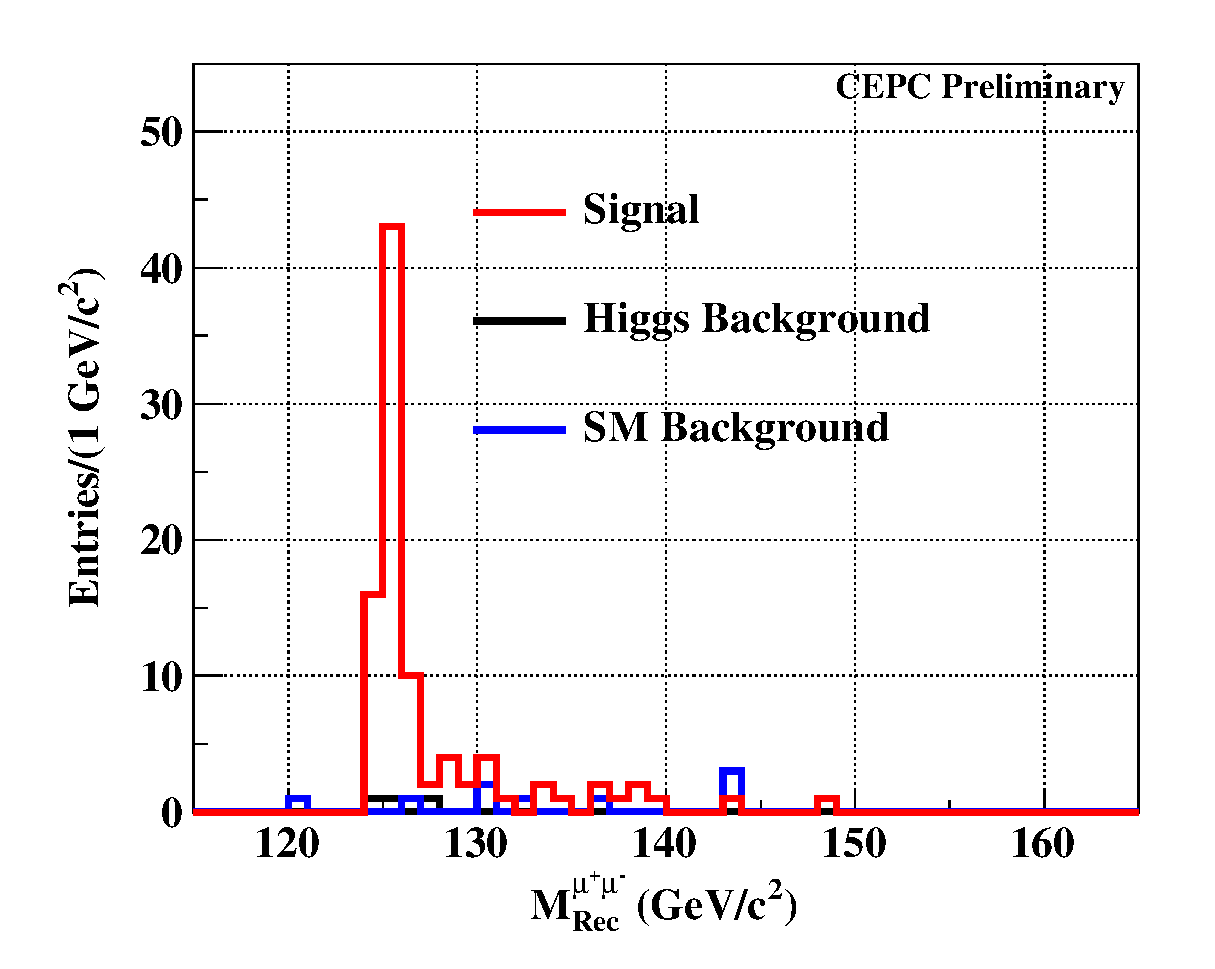
\includegraphics[width=0.5\textwidth]{e2e2H/evuv/uuh_recfit}
\caption[]{The distribution of recoil mass of $\mu^+\mu^-$ after event selection}
\label{fig:uuhevuvrecfit}
\end{figure}

The final number of signal events is estimated to be $N_{sig} = 93\pm10$ 
with a selection efficiency of $\varepsilon = 54.1\%$. 
Hence, the expected sensitivity of the measurement for this channel is:
\begin{equation*}
Accu.=\frac{\sqrt{S+B}}{S} = 10.7\%.
\end{equation*}

\subsection{Analysis of $e^+e^-\rightarrow ZH, Z\rightarrow e^+e^-, H\rightarrow WW^*, WW^*\rightarrow \mu\nu q\bar{q}$ decay}
\subsubsection{Event selection}
This channel is more promising for a high precision measurement compared to
the $ZWW^*\to \mu\mu\mu\nu  e\nu$ channel  discussed in the previous section
due to the larger branching ratios involved.
The final state consists of three leptons, several jets and neutrinos.
The fully leptonic decay background {\color{blue} and full hadronic decay} can be reduced a lot
by requiring the number of remain particles, {\color{blue}$7 < N_{Remain} < 30$, except for three energetic leptons}.

In this final state, the most effective criteria to supress the
SM background in  pre-selection are the invariant mass and the recoil mass 
of the $ee$ system. The constraints $80\gev/c^2 < M_{Inv}^{e^+e^-} < 100\gev/c^2$
and $120\gev/c^2 < M_{Rec}^{e^+e^-} < 150\gev/c^2$ are, hence, required, as part
of the channel pre-selection.

Differences in the di-jet system between Higgs, $W$ and $Z$ boson deacys
as well as hadroni $\tau$ lepton decays can be exploited to reduce backgrounds.
In particular, the invariant mass of the di-jet system is required to be
$10\gev/c^2 < M_{Rec}^{di-Jet} < 95\gev/c^2 $. In addition, $b$-tagging is used
to veto backgrounds with $b$-jets.

The excellent expected CEPC tracking performance is exploited to
distinguish muons from $W$  and muons from $\tau$ lepton decays
using the requirement 
$\sqrt{(\frac{D_{0}}{sigD_{0}})^2+(\frac{Z_{0}}{sigZ_{0}})^2} < 4$.
In addition, in order to veto background from the $t$-channel
{\color{blue}because there are lots of $t$-channel background according to Feynman diagram, }
a transverse momentum requirement $p_T > 5\gev$ is applied.

\begin{figure}[H]
\centering
	\subfigure[]{
		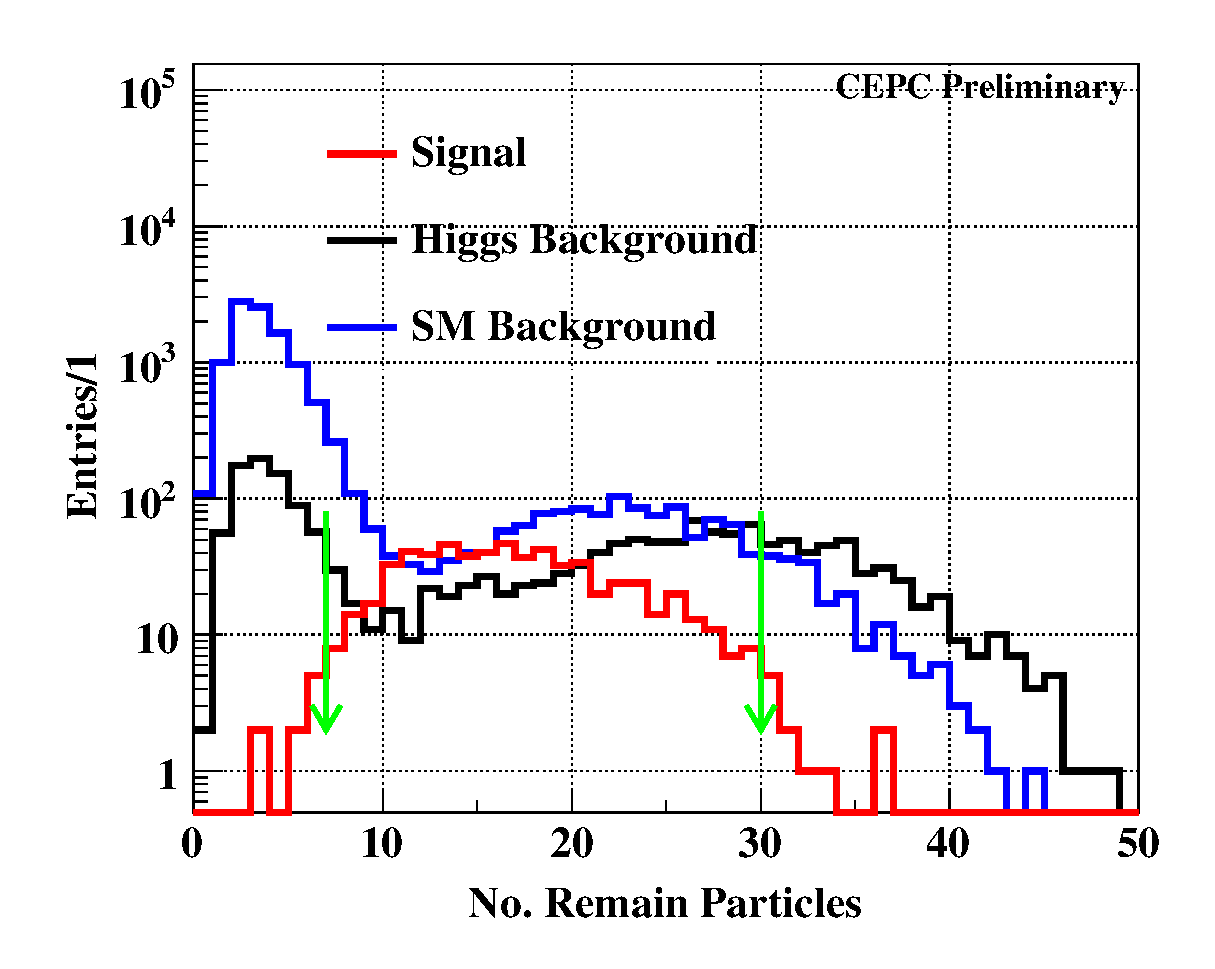
\includegraphics[width= 0.35\textwidth]{e1e1H/uvqq/nRem}
		\label{fig:eeuvqqRem}
	}
\subfigure[]{
	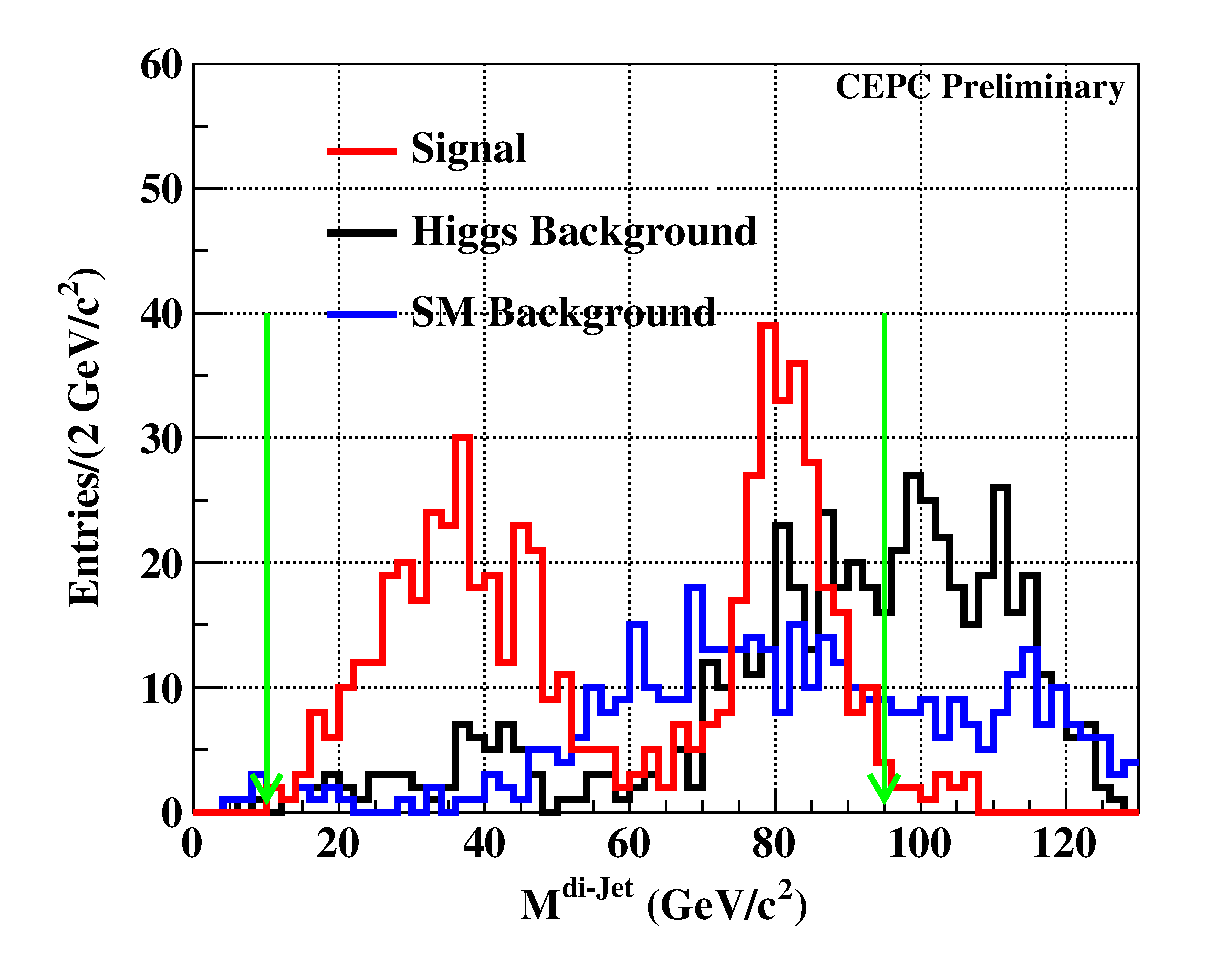
\includegraphics[width= 0.35\textwidth]{e1e1H/uvqq/diJet_InvMass}
	\label{fig:eeuvqqInvJet}
}
\subfigure[]{
	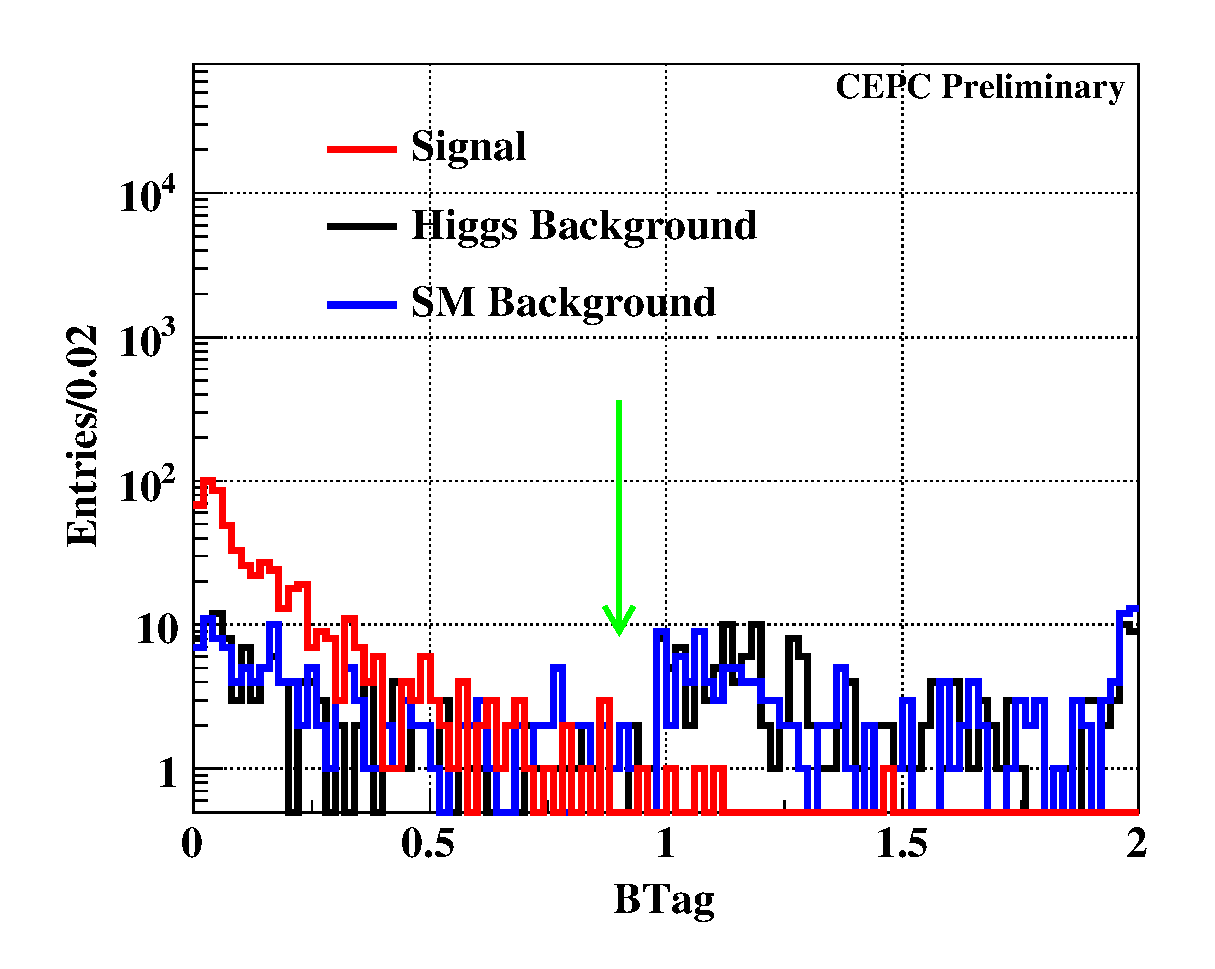
\includegraphics[width= 0.35\textwidth]{e1e1H/uvqq/Btag}
	\label{fig:eeuvqqBtag}
}
\subfigure[]{
	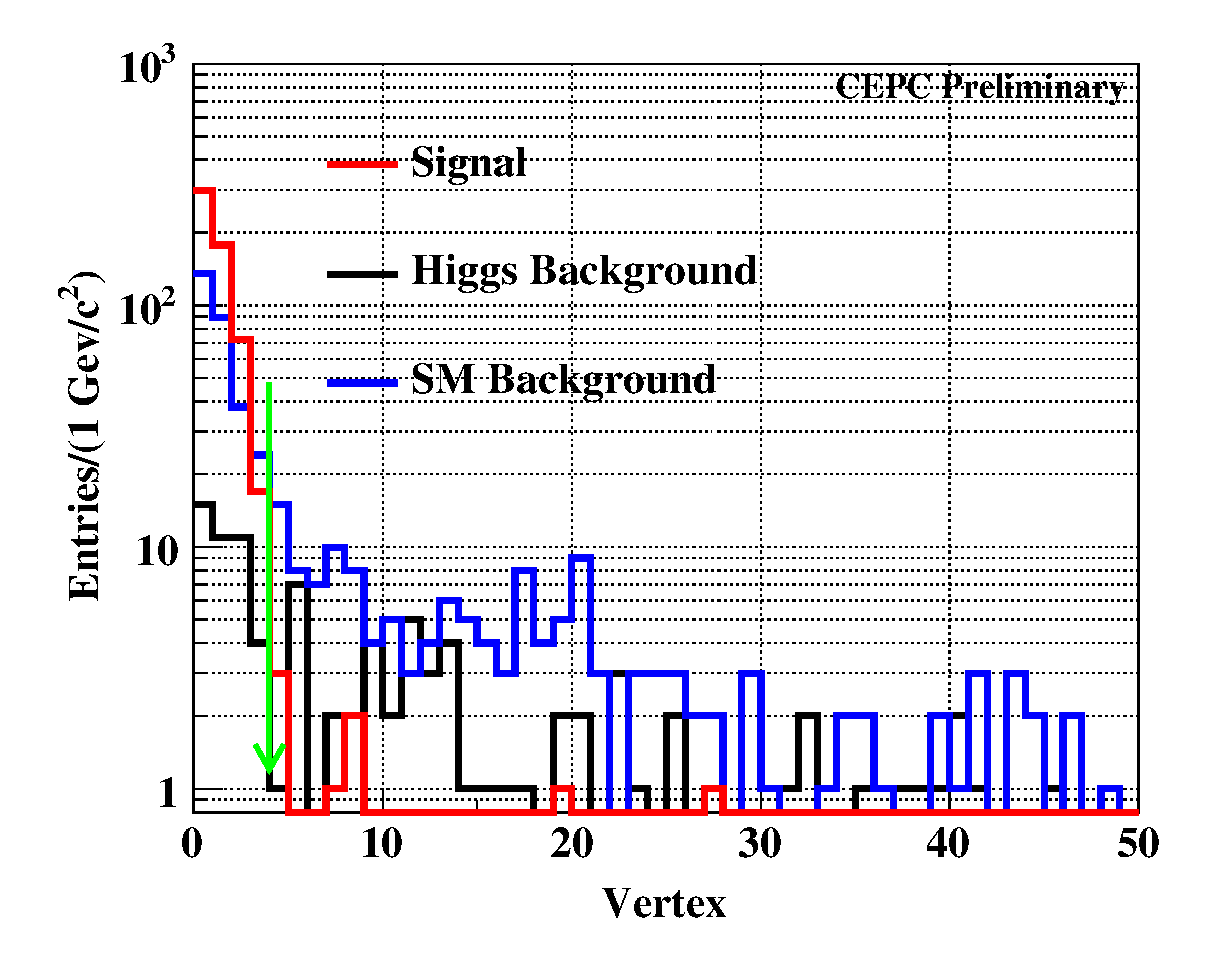
\includegraphics[width= 0.35\textwidth]{e1e1H/uvqq/Vertex}
	\label{fig:eeuvqqVertex}
}
\subfigure[]{
	\includegraphics[width=0.35\textwidth]{e1e1H/uvqq/Pt}
	\label{fig:eeuvqqPt}
}
\caption[]{
	\ref{fig:eeuvqqRem} The No. remain particles of $e^+e^-\rightarrow ZH, Z\rightarrow e^+e^-, H\rightarrow WW^*,  
	WW^*\rightarrow \mu\nu q\bar{q}$ decay. 
	Because it is semi-leptonic decay channel, so the No. remain particles should between it of hadronic decay and full-leptonic decay.
	\ref{fig:eeuvqqBtag} The distribution of Btag, we plus the Btag value of each jets because of existing two jets. And because no $b$-jet 
	decay from $W$ boson, the value of them should be less than 1.
	\ref{fig:eeuvqqVertex} The distribution of vertex of lepton. Leptons from $\tau$ and $b$-jet would fly a long distance, 
	so they would be rejected effectively.
	\ref{fig:eeuvqqPt} The distribution of transverse momentum $p_T$. Transverse momentum of t channel would be lower than of s channel.
	\ref{fig:eeuvqqInvJet} The distribution of di-jet invariant mass, the high-side could distinguish the jets from $Z$ boson or $H$ boson.
	}
\label{fig:eeuvqqfourcut}
\end{figure}

The selection criteria, as well as the signal and background events
passing each of them, are summarized in in Table~\ref{tab:eeuvqqCutchain}.
The main backgrounds after the full selection are shown in Table~\ref{tab:uuuvqqbkg}, 
{\color{blue}and only background which remain number is larger than ten would be regarded as main background}.
\begin{table}[H]
  \begin{center}
    \begin{tabular}{ccccc}
      \hline \hline
      \multicolumn{1}{c}{Category} & \multicolumn{1}{c}{Signal}&\multicolumn{1}{c}{$ZH$} background&\multicolumn{1}{c}{SM background}\\ 
      \hline
      Total 	      	 									&   1149	& 36319	& 1303847\\
      $N_{ZPole}=2; N_{Isolep}=1; N_{Jets} =2; l = \mu$		&   1022	& 1970	& 21857\\
	  Validation of pre-selection					   		&   631 	& 1207	& 2987\\
	  $7 < N_{Remain} < 30$									&	603		& 540	& 436\\
	  $15\gev/c^2 < M_{Rec}^{di-Jet} < 95\gev/c^2 $			&	589		& 284	& 278\\
	  $Btag < 0.9$											&	584		& 116	& 131\\
	  $M_{Missing} < 45\gev/c^2$							&   571		& 72	& 102\\
	  $\sqrt{(\frac{D0}{sigD0})^2+(\frac{Z0}{sigZ0})^2} < 4$&	564  	& 23 	& 45\\
	  $p_T > 5\gev$											&	551		& 18	& 21	\\	
      \hline \hline
    \end{tabular}
  \caption[Monte Carlo purities in the single lepton sample]{% Monte
    The final event selection of $e^+e^-\rightarrow ZH, Z\rightarrow e^+e^-, H\rightarrow WW^*, WW^*\rightarrow \mu\nu q\bar{q}$ decay}
  \label{tab:eeuvqqCutchain}
  \end{center}
\end{table}
\begin{table}[H]
\begin{center}
\begin{tabular}{lrc}
\hline\hline
Decay Chain	& Final States 	&	Number of Events	\\
\hline
$e^+e^-\rightarrow ZH, Z\rightarrow e^+e^-, H\rightarrow WW^*\rightarrow \tau\nu q\bar{q}$ & $e^+, e^-, \tau, \nu, 2q $	&	14\\
$e^+e^-\rightarrow e^+e^-Z, Z\rightarrow qq$ 					& $e^+, e^-, 2q$								&	13\\
\hline\hline
\end{tabular}
\caption{Summery of total background with the same final states of signal event}
\label{tab:uuuvqqbkg}
\end{center}
\end{table}

\subsubsection{Statistical result}
After selection, the distribution of the recoil mass of the $e^+e^-$ system is shown in Figure~\ref{fig:eehuvqqrecfit}.
\begin{figure}[H]
\centering
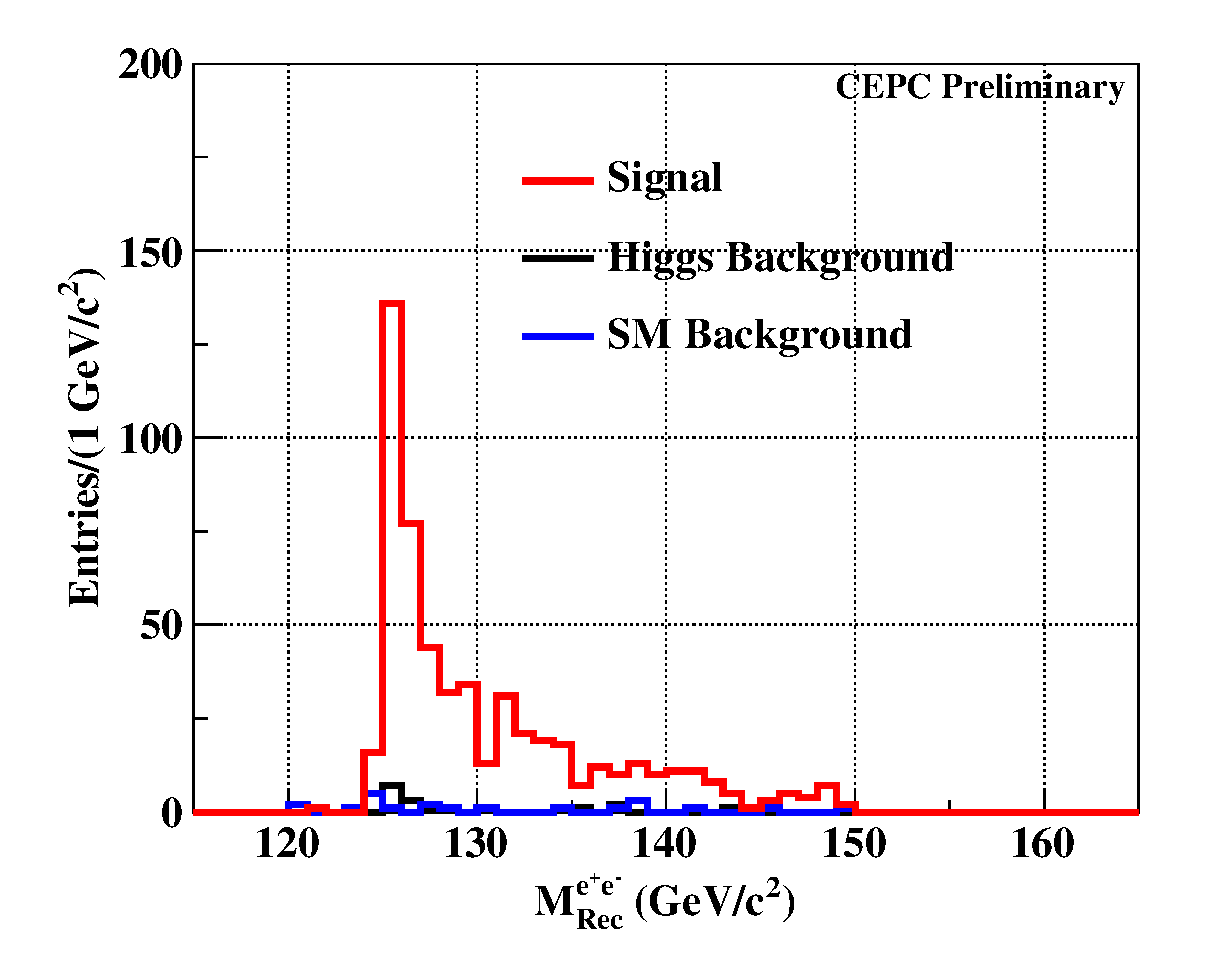
\includegraphics[width=0.5\textwidth]{e1e1H/uvqq/fit_RecMass}
\caption[]{The distribution of recoil mass of $e^+e^-$ after event selection}
\label{fig:eehuvqqrecfit}
\end{figure}

The final number of signal events is found to be $N_{sig} = 551\pm24$
and the selection efficiency is $\varepsilon = 48.0\%$. 
Hence, the expected sensitivity of the measurement for this channel is:
\begin{equation*}
Accu.=\frac{\sqrt{S+B}}{S} = 4.5\%.
\end{equation*}

\subsection{Analysis of $e^+e^-\rightarrow ZH, Z\rightarrow \nu\bar{\nu}, H\rightarrow WW^*, WW^*\rightarrow q\bar{q}q\bar{q}$ decay}
\subsubsection{Event selection}
This is a hadronic channel that features no leptons, light flavour jets
and large missing transverse energy. The SM background is
reduced by vetoing events with isolated leptons and by requiring at
least two jets. The event particle multiplicity is required to be large,
$N_{\mathrm{Particles}}^{\mathrm{Total}} > 20$, due to the many hadrons produced
after the quark hadronization takes place.
\begin{figure}[H]
	\centering
	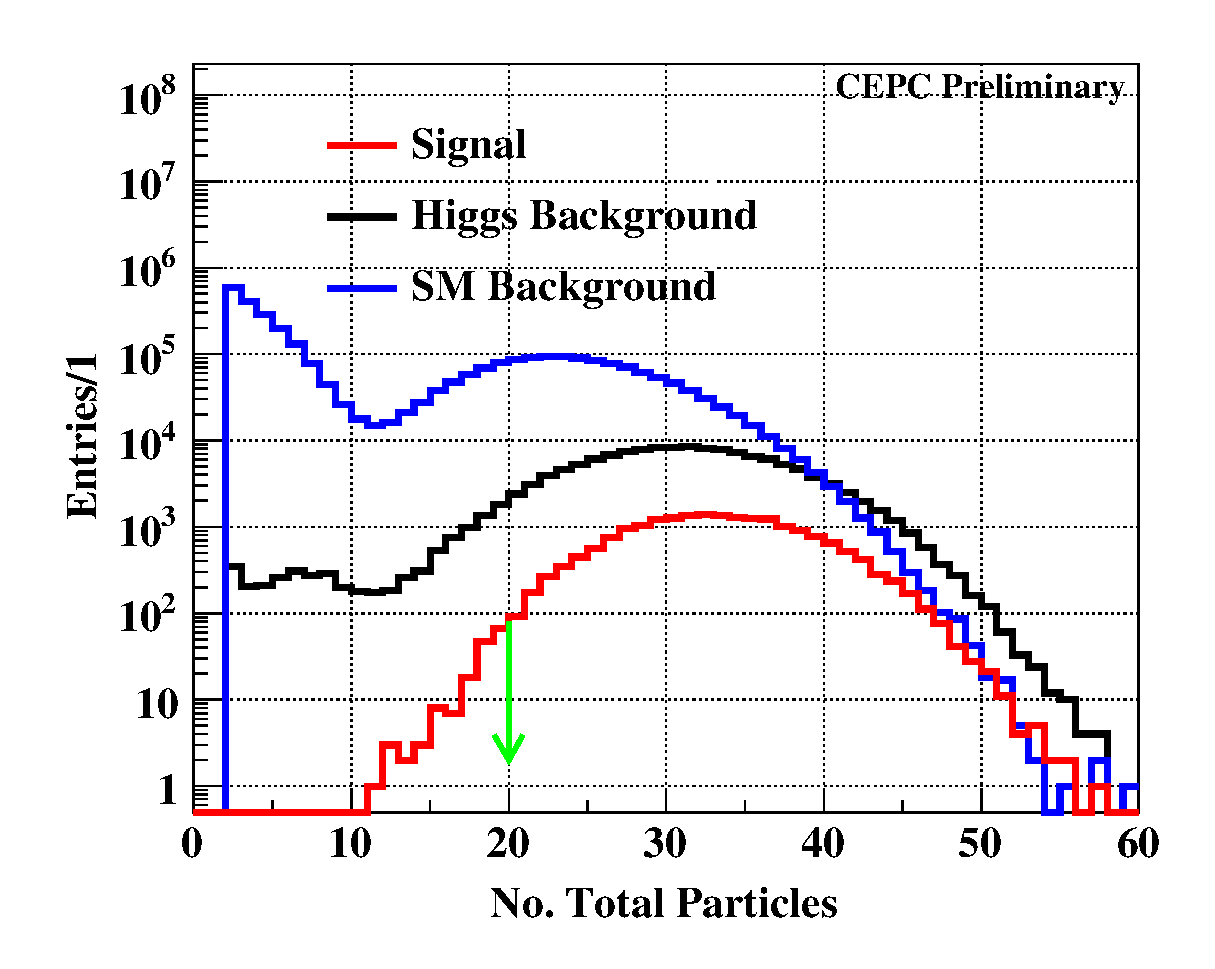
\includegraphics[width= 0.35\textwidth]{nnH/fourq/TotPart}
	\label{fig:nnH4qTotPart}
	\caption[]{The number of total final particles distribution. To count the total number, the energy threshold of each particle 
	is required, $E > 1\gev$}
\end{figure}

{\color{red}[It is not clear how this process is done, please clarify.(\color{blue} just do jet clustering twice.)]}
For this study, jet selection is done in two steps. In the first step,
two jets are required in the event to discriminate against 
two-jet background, such as $H\rightarrow q\bar{q}$ decays, 
$ZZ$ semi-leptonic decays and single-$Z\nu$ semi-leptonic decays. 
The jets jets are required to satisfy $Btagging < 0.9$, 
$Cos\theta_{2jets} > 0.87$ and $\Sigma|M_{Inv}^{2jet}| > 50\gev/c^2$. 
{\color{blue} $Btagging$ means the probilities of flavor tagging for each jet and sum them up. 
$Cos\theta_{2jets} $ means the cos angle of this two jets.
$\Sigma|M_{Inv}^{2jet}|$ means sum the invariant mass of each jet.}
In the second step, four jets are required in the event. This category
is more important, since it is the feature of the signal. 
The event is required to satisfy  $Y_{34} > 0.005$, which ycut~\cite{Catani:1991hj} means the distances between all jets i and j.
Subsequently, the four jets are used to form all possible jet pairs and the
jet-jet system invariant mass is examined. The jet-jet pair with invariant
 mass closest to the $W$ boson mass is taken as the on-shell $W$ boson decay
of the signal decay chain. The remaining two jets are assigned to the
off-shell $W$ boson decay. The invariant mass distribution of the two
jet-jet pairs is shown in Figure~\ref{fig:nnHfourqFMass}.
In addition, the following conditions are required to be met by the jet-jet pairs:
\begin{itemize}
	\item $ 65\gev/c^2 < M_{Inv}^{Real4jet} < 85\gev/c^2$, 
	\item $ 15\gev/c^2 < M_{Inv}^{Virt4jet} < 50\gev/c^2$, 
	\item $ M_{Inv}^{Virt4jet} > -7/3\dot M_{Inv}^{Real4jet} + \frac{605}{3}\gev/c^2$,
\end{itemize}
where $M_{Inv}^{Real4jet}$  ($M_{Inv}^{Virt4jet}$) is the invariant mass of the jet-jet system assigned to the on-shell (off-shell) $W$ boson decay.
\begin{figure}[H]
	\centering
	\subfigure[]{
		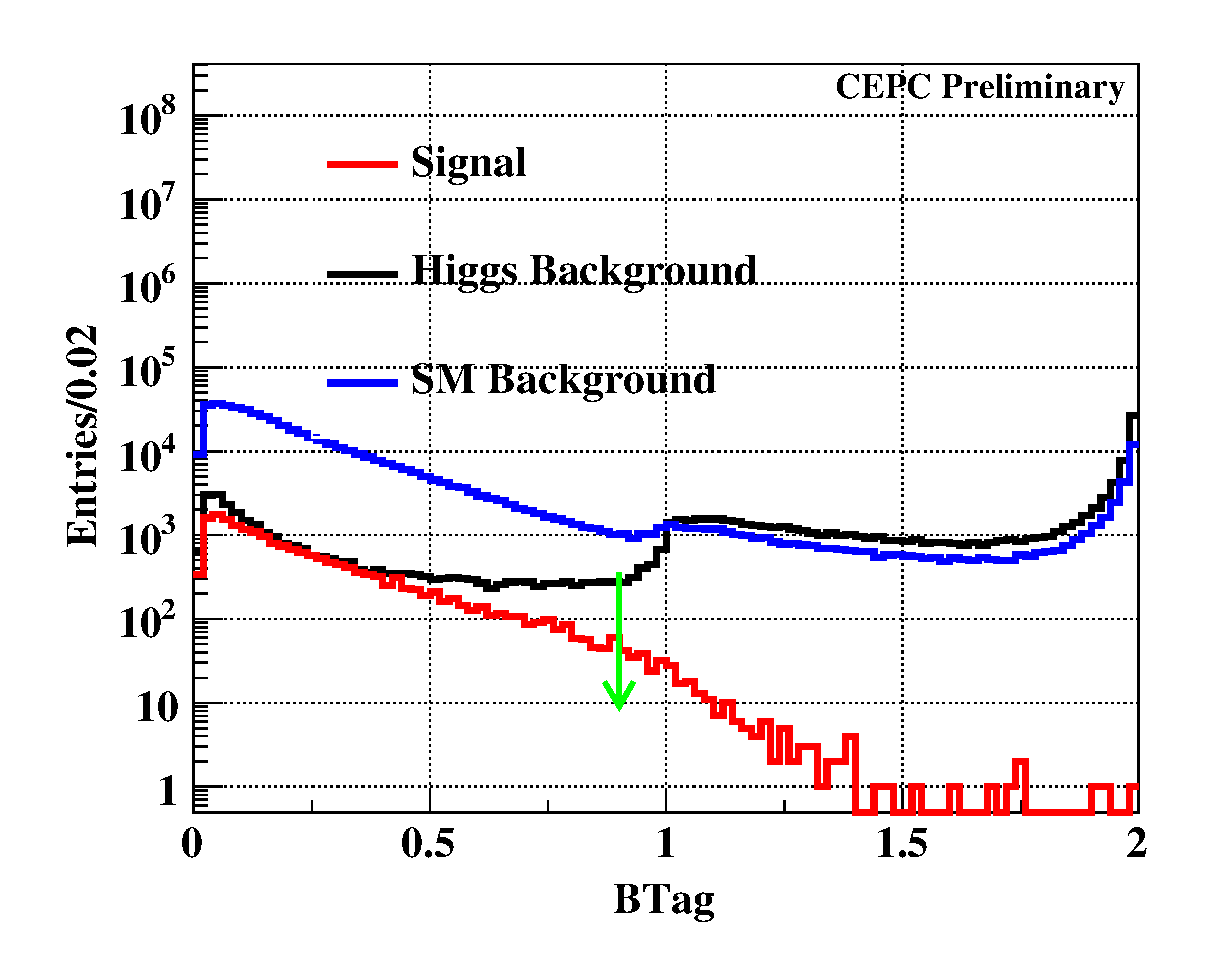
\includegraphics[width= 0.35\textwidth]{nnH/fourq/Btag}
		\label{fig:nnHfourqBtag}
	}
	\subfigure[]{
		\includegraphics[width= 0.35\textwidth]{nnH/fourq/TwoJetsAngle}
		\label{fig:nnHfourqTJAngle}
	}
	\subfigure[]{
		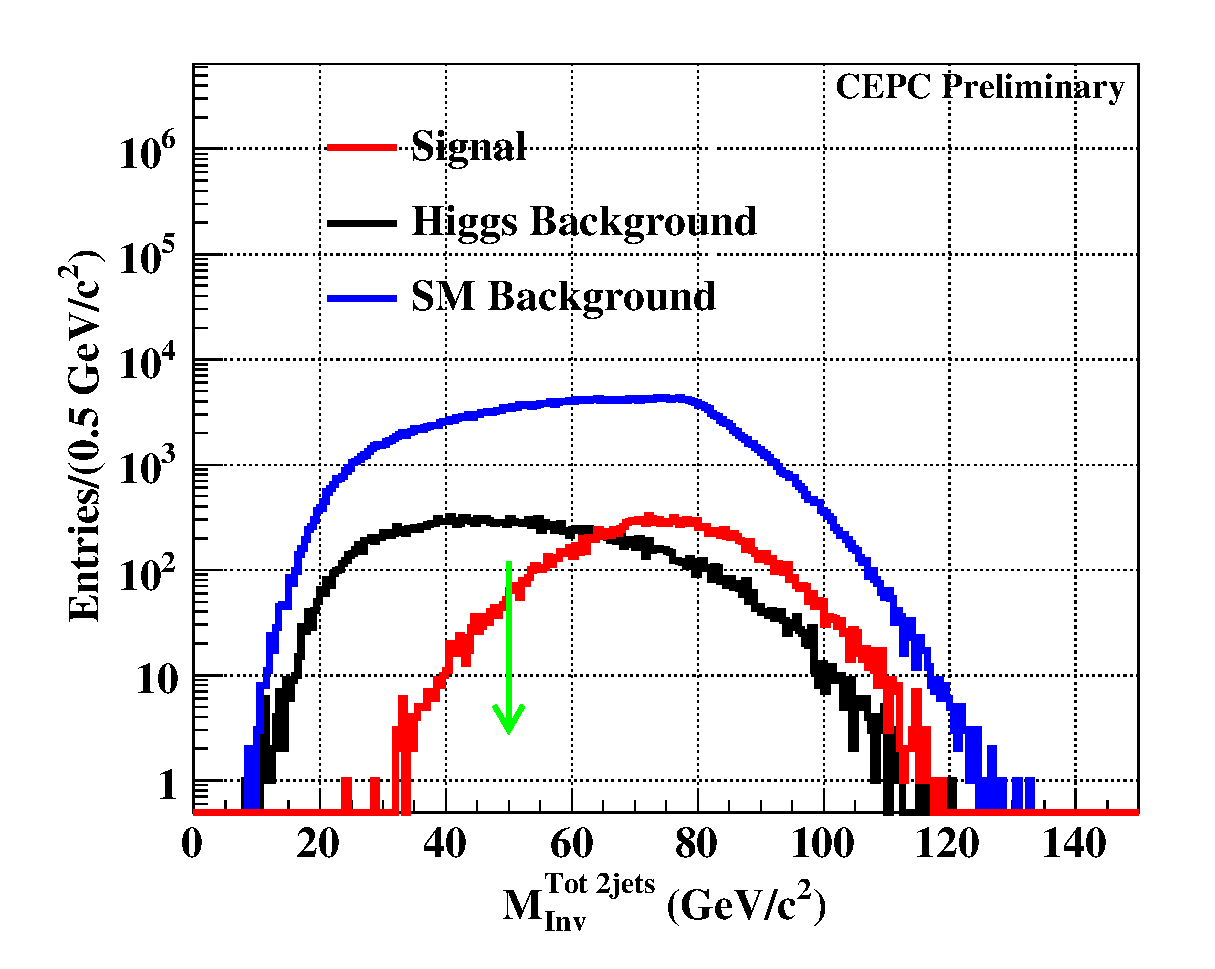
\includegraphics[width= 0.35\textwidth]{nnH/fourq/tjet_TotMass}
		\label{fig:nnHTJPInvMass}
	}
	\caption[]{
		\ref{fig:nnHfourqBtag} B-tag of two jets distribution. We plus the value of B-tag of each jet, 
		\ref{fig:nnHfourqTJAngle} The distribution of angle between two jets. The boost of Higgs is larger, so the angle 
		between two jets in signal should be smaller its in background. 
		\ref{fig:nnHTJPInvMass} The distribution of total invariant mass of two jets. The number of jets in almost background is two. 
		The invariant mass of each jet should be smaller.}
	\label{fig:nnHfourqTwoJet}
\end{figure}
\begin{figure}[H]
	\centering
	\subfigure[]{
		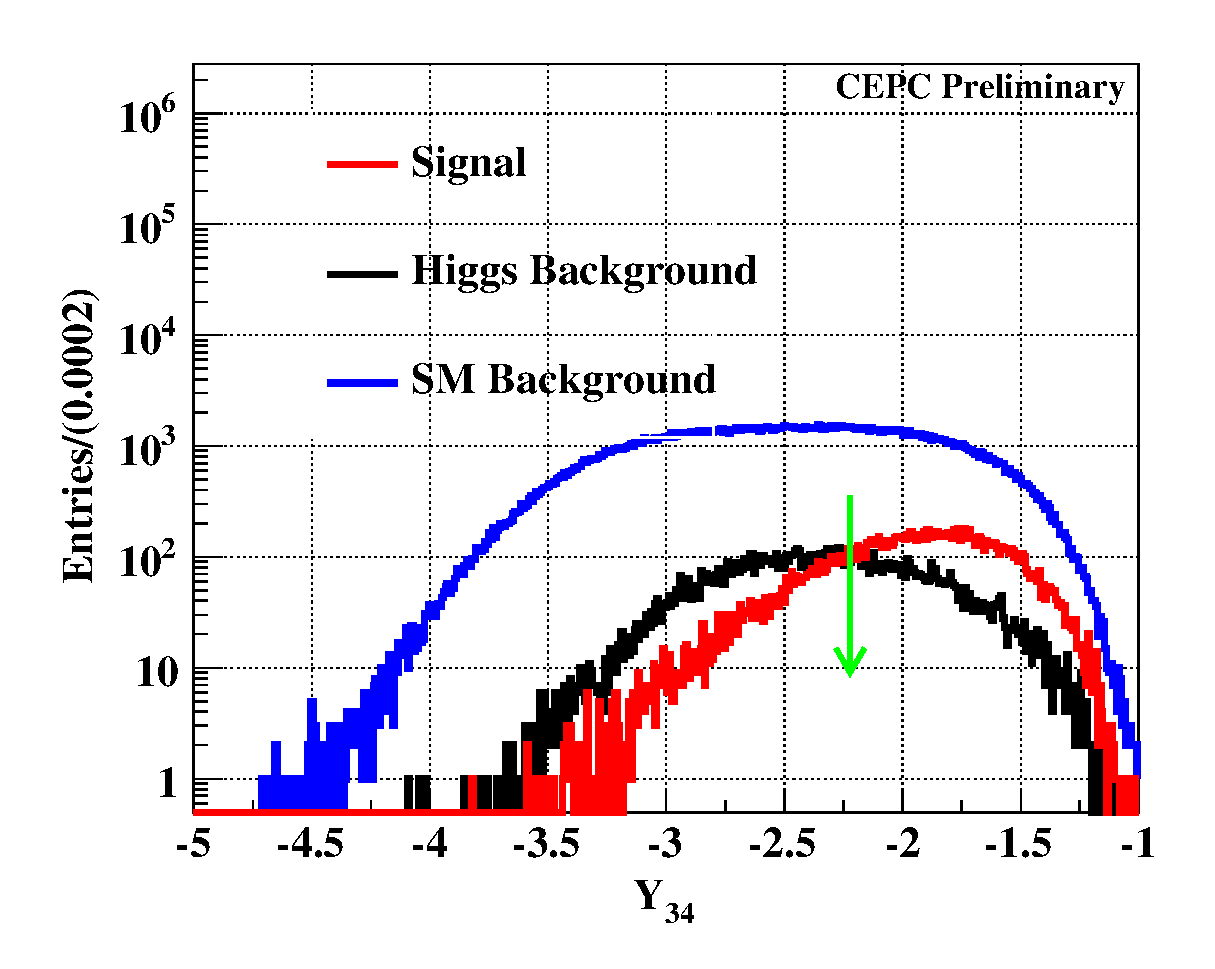
\includegraphics[width=0.35\textwidth]{nnH/fourq/Y34}
		\label{fig:nnHfourqY34}
	}
	\subfigure[]{
		\includegraphics[width=0.7\textwidth]{nnH/fourq/4qInvMass}
		\label{fig:nnHfourqFMass}
	}
	\caption[]{
		\ref{fig:nnHfourqY34} Y value distribution. 
		\ref{fig:nnHfourqFMass} 2D scatter diagram of invariant mass of real and virtual $W$ boson. The left plot represents the distribution 
		of signal, and the right is of background. In order to distinguish the signal and background effectively, a hexagonal mass window is 
		applied.}
	\label{fig:nnHfourqFourJet}
\end{figure}
%%%%%%%%%%%%%%%%%%%%%%%%%%%%%%%%%%%%%%% nn qqqq %%%%%%%%%%%%%%%%%%%%%%%%%%%%%%%%%%%%%%%%%%%%%%%

The event selection steps as well as the number of signal and background
events passing each step is shown in Table~\ref{tab:nnHfourqcutchain}.
The signal efficiency for this selection is about 50\%.
\begin{table}[H]
  \begin{center}
    \begin{tabular}{cccccccc}
      \hline \hline
      \multicolumn{1}{c}{Category}      & \multicolumn{1}{c}{Signal}&\multicolumn{1}{c}{$ZH$ background}&\multicolumn{1}{c}{SM background}\\ 
      \hline
      Total 	      	 					&   23938& 208200&	21314314	\\
	  Validation of pre-selection		  	&   20405& 143765&	3166923	\\
	  $N_{Particle}^{Tot} > 20$				&	19681& 124112& 	537839	\\
	  $Btag < 0.9$							&	19349& 28857 & 	477099	\\
	  $Cos\theta_{2jets} > 0.87  $			&	19298& 28673 &	433563	\\
	  $\Sigma|M_{Inv}^{2jet}| > 50\gev$		&   18621& 14793 &	309919	\\
	  $Y_{34} > 0.005$						&	15183& 6919  &  122866	\\
	  Combined Variable						&	9022 & 3075  &	38226	\\
      \hline \hline
    \end{tabular}
  \caption[Monte Carlo purities in the single lepton sample]{% Monte
  The final event selection of $e^+e^-\rightarrow ZH, Z\rightarrow \nu\bar{\nu}, H\rightarrow WW^*, WW^*\rightarrow q\bar{q}q\bar{q}$ decay}
  \label{tab:nnHfourqcutchain}
  \end{center}
\end{table}
\begin{table}[H]
\begin{center}
\begin{tabular}{lrc}
\hline\hline
Decay Chain	& Final States 	&	Number of Events\\
\hline
$e^+e^-\rightarrow ZH, Z\rightarrow \nu\bar{\nu}, H\rightarrow c\bar{c}$ & $\nu, \bar{\nu}, c, \bar{c}$			&192	\\
$e^+e^-\rightarrow ZH, Z\rightarrow \nu\bar{\nu}, H\rightarrow b\bar{b}$ & $\nu, \bar{\nu}, b, \bar{b}$			&352	\\
$e^+e^-\rightarrow ZH, Z\rightarrow \nu\bar{\nu}, H\rightarrow gg$ 		 & $\nu, \bar{\nu}, 2g		  $			&2028	\\
$e^+e^-\rightarrow ZH, Z\rightarrow \nu\bar{\nu}, H\rightarrow ZZ^*, ZZ^*\rightarrow q\bar{q}q\bar{q}$ &
																$\nu, \bar{\nu}, 2q, 2\bar{q}$&		439\\	
$e^+e^-\rightarrow ZZ, ZZ\rightarrow \nu\bar{\nu}q\bar{q}$      & $\nu, \bar{\nu}, 2q$					&3115	\\
$e^+e^-\rightarrow ZZ, ZZ\rightarrow \tau^+\tau^-q\bar{q}$ 		& $\tau^+, \tau^-, 2q$					&910	\\
$e^+e^-\rightarrow WW, WW\rightarrow \tau\nu qq$     		   	& $\tau, \nu, 2q$						&	30398\\
$e^+e^-\rightarrow WW, WW\rightarrow \mu\nu qq$        			& $\mu, \nu, 2q$						&	277\\
$e^+e^-\rightarrow \nu\bar{\nu} Z, Z\rightarrow qq$ 			& $\nu, \bar{\nu}, 2q$					&	1838\\
$e^+e^-\rightarrow e\nu W, W\rightarrow e\nu qq$        		& $e, \nu, 2q$							&	1398\\
$e^+e^-\rightarrow qq$											& $2q$											&262 \\
\hline\hline
\end{tabular}
\caption{Summery of main background with the same final states of signal event}
\label{tab:nnqqqqbkg}
\end{center}
\end{table}

\subsubsection{Statistical result}
The missing mass distribution after the selection is shown in
 Figure~\ref{fig:nnhqqqqmismass}.
\begin{figure}[H]
\centering
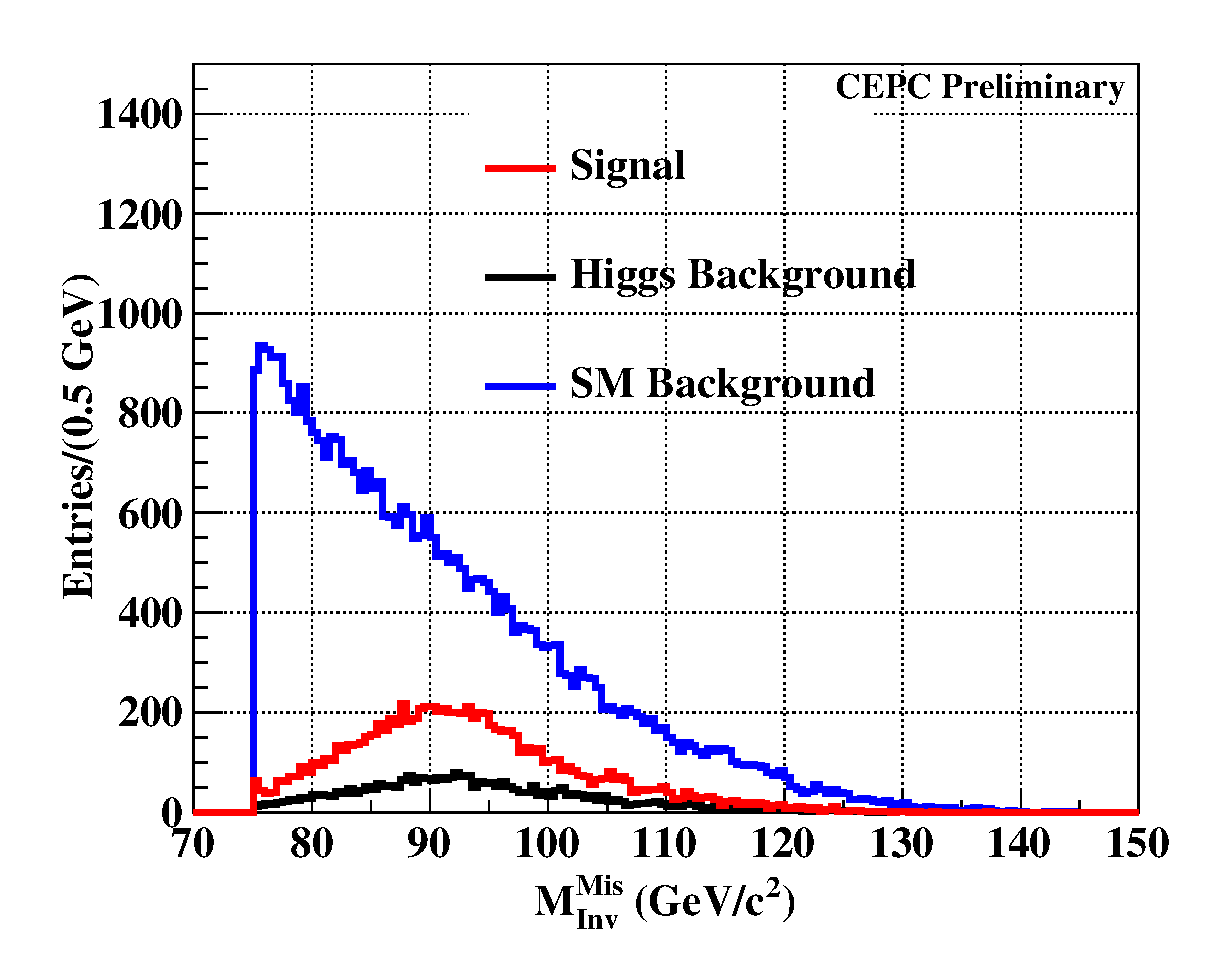
\includegraphics[width=0.5\textwidth]{nnH/fourq/MisMass_AF}
\caption[]{The distribution of recoil mass of missing mass of event after event selection}
\label{fig:nnhqqqqmismass}
\end{figure}

The final number of signal events is found to be $N_{sig} = 9022\pm224 $
and the signal efficiency is $\varepsilon = 37.7\%$. 
Hence, the expected sensitivity of the measurement for this channel is:
\begin{equation*}
Accu.=\frac{\sqrt{S+B}}{S} = 2.5\%.
\end{equation*}

%
%%%%%%%%%%%%%%%%%%%%%%%%%%%%%%%%%%%%%%%%%%%%%%%%%%%%%%%%%%%%%%%%%%%%%%%%%%%%%%%
% Data characteristics
%%%%%%%%%%%%%%%%%%%%%%%%%%%%%%%%%%%%%%%%%%%%%%%%%%%%%%%%%%%%%%%%%%%%%%%%%%%%%%%
%
%\section{Data characteristics}



%
%%%%%%%%%%%%%%%%%%%%%%%%%%%%%%%%%%%%%%%%%%%%%%%%%%%%%%%%%%%%%%%%%%%%%%%%%%%%%%%
% Systematic uncertainties
%%%%%%%%%%%%%%%%%%%%%%%%%%%%%%%%%%%%%%%%%%%%%%%%%%%%%%%%%%%%%%%%%%%%%%%%%%%%%%%
%
%\section{Systematic uncertainties}

%Give a detailed list of systematic uncertainties, the method
%by which they were obtained, and a justification of the resulting
%values.
%%
%Use ``systematic uncertainty'' instead of ``systematic errors''.
%The latter sounds as if you have made a mistake systematically.

%
%%%%%%%%%%%%%%%%%%%%%%%%%%%%%%%%%%%%%%%%%%%%%%%%%%%%%%%%%%%%%%%%%%%%%%%%%%%%%%%
% Results
%%%%%%%%%%%%%%%%%%%%%%%%%%%%%%%%%%%%%%%%%%%%%%%%%%%%%%%%%%%%%%%%%%%%%%%%%%%%%%%
%
\section{Results}
%\subsection{Statistical uncertainty}
The final result of precision for the branching ratio BR($H\rightarrow WW^*$) is 
obtained using the relation: 
\begin{equation*}
\Delta{Br(H\rightarrow WW^*)}/Br(H\rightarrow WW^*) = 
\sqrt{(\frac{\Delta N_{obs.}}{N_{obs.}})^2
		+(\frac{\Delta N_{total}}{N_{total}})^2
	+(\frac{\Delta Br_{rel.}}{Br_{rel.}})^2},
\end{equation*}
where $N_{total}$ and $\Delta N_{total}$ are the total number of $ee\to ZH$ producted events and its deviation,
$N_{obs.}$ and $\Delta N_{obs.}$ are the number of signal events after selection and its deviation in this sample,
and finally, $Br_{rel.}$ and $\Delta Br_{rel.}$ included branch fraction of $Z$ boson and $W$ boson and its deviation
which are given by PDG table~\cite{Agashe:2014kda} and listed in Table~\ref{tab:relativeresult}. And these precisions are neligible, 
therefore a equation would be got:
\begin{equation}
	\Delta{Br(H\rightarrow WW^*)}/Br(H\rightarrow WW^*) \sim \sqrt{(\frac{\Delta N_{obs.}}{N_{obs.}})^2}.
	\label{equ:one}
\end{equation}
Then, define the vairable $\Gamma_i$ as the precision of each subchannel, $\Gamma_{ij}$ as the combination of two subchannels. 
The result of combination is:
\begin{equation}
	\Gamma_{ij}^2 = \frac{\Gamma_i^2\Gamma_j^2}{\Gamma_i^2+\Gamma_j^2}.
	\label{equ:two}
\end{equation}

The relative uncertainty for the number of signal events is shown in Table~\ref{tab:fullstatistic}. 
\begin{table}[H]
  \begin{center}
    \begin{tabular}{cr@{$\pm$}lcc}
      \hline \hline
      Category&\multicolumn{2}{c}{Signal}&\multicolumn{1}{c}{Relative uncertainty}&\multicolumn{1}{c}{Efficiency of selection}\\ 
      \hline
      $Z\rightarrow e^+e^-; H\rightarrow WW^*\rightarrow e\nu e\nu			$	&20    &7	&35.0\% &25.0\%\\
      $Z\rightarrow e^+e^-; H\rightarrow WW^*\rightarrow \mu\nu\mu\nu		$	&44    &8	&18.2\%	&43.1\%\\ 
      $Z\rightarrow e^+e^-; H\rightarrow WW^*\rightarrow e\nu\mu\nu			$	&53    &8	&15.1\% &27.6\%\\
	  $Z\rightarrow e^+e^-; H\rightarrow WW^*\rightarrow e\nu qq			$	&435   &23  &5.3\%  &37.0\%\\
	  $Z\rightarrow e^+e^-; H\rightarrow WW^*\rightarrow \mu\nu qq			$	&551   &24	&4.5\%  &48.0\%\\
      $Z\rightarrow \mu^+\mu^-; H\rightarrow WW^*\rightarrow e\nu e\nu		$	&23    &5	&21.7\% &25.8\%\\
      $Z\rightarrow \mu^+\mu^-; H\rightarrow WW^*\rightarrow \mu\nu\mu\nu	$	&39    &7	&17.9\%	&44.8\%\\ 
      $Z\rightarrow \mu^+\mu^-; H\rightarrow WW^*\rightarrow e\nu\mu\nu		$	&93    &10	&10.7\% &54.1\%\\
	  $Z\rightarrow \mu^+\mu^-; H\rightarrow WW^*\rightarrow e\nu qq		$	&573   &25  &4.0\%  &51.7\%\\
	  $Z\rightarrow \mu^+\mu^-; H\rightarrow WW^*\rightarrow \mu\nu qq		$	&756   &30	&4.4\%  &68.4\%\\
	  $Z\rightarrow \mu^+\mu^-; H\rightarrow WW^*\rightarrow qqqq			$	&   	&	&2.9\%  &\\
	  $Z\to \nu\bar{\nu}; H\to WW^* \to e \nu qq							$	&680   &32	&4.7\%	&9.8\%\\
	  $Z\to \nu\bar{\nu}; H\to WW^* \to \mu\nu qq							$	&790   &43	&4.2\%	&11.2\%\\
	  $Z\rightarrow \nu\bar{\nu}; H\rightarrow WW^*\rightarrow qqqq			$	&9022  &224	&2.5\%  &37.7\%\\
      \hline \hline
    \end{tabular}
  \caption{Statistic uncertainty of Signal and Relative uncertainty}
  \label{tab:fullstatistic}
  \end{center}
\end{table}
\begin{table}[H]
\begin{center}
\begin{tabular}{cccccc}
\hline\hline
&Total events $N$ & $Br(W\rightarrow \ell\nu)$ & $Br(W\rightarrow qq)$ & $Br(Z\rightarrow \ell^+\ell^-)$ & $Br(Z\rightarrow qq)$\\
\hline
Mean value	&1060000		 &  10.86\%				 &  67.41\%			   &  3.3658\%				  &  69.91\%			\\
Uncertainty	&$\pm4000$		 &	$\pm0.09\%$			 &  $\pm0.27\%$		   &  $\pm0.0023\%$			  &  $\pm0.06\%$			\\
\hline\hline
\end{tabular}
\caption[]{Relative data for measurement of branch ratio}
\label{tab:relativeresult}
\end{center}
\end{table}

Through applied the Equ~\ref{equ:one} and Equ~\ref{equ:two}, he overall combination results in a statistical uncertainty for 
$\Delta{Br(H\rightarrow WW^*)}/Br(H\rightarrow WW^*)$ is 1.29\%.

%\subsection{Systematic uncertainty}
%Because the data we have used are MC data, the analysis of systematic uncertainty should be based on a experienced discussion. 
%And we can refer to the result of LEP due to it is also a electron positron collider.
%\begin{itemize}
%\item Tracker reconstruction: Especially for reconstruction of lepton, it is a main resource of systematic uncertainty. 
%Improving the efficiency of reconstruction would reduce the uncertainty, and we should do research systematically in the future.
%\item Jet clustering: It would be a main influence for measurement of mass of $W$ boson. Energy resolution of jet and flavor tag 
%are two parts of this systematic uncertainty.
%\item MC simulation: In true practice, MC would not match the data totally, so we should reduce the bias between MC and data to 
%decrease this systematic uncertainty when we have true data sample.
%\item Measurement of luminosity: The luminosity of CEPC is given by measurement of BaBar scatter. This measurement would 
%has its own uncertainty, so it is also a resource of systematic uncertainty.
%\end{itemize}
%

%\subsection{Measurement of Higgs width}
%As mentioned before, $\Gamma_H = \frac{Y_1^2 Y_3 F_2 F_4}{F_1^2 F_3 Y_2 Y_4} = f_a\times\frac{\sigma_{\nu\bar{\nu}H}}{Br(H\rightarrow WW^*)}$, 
%and $f_a= \frac{F_2 F_4}{F_1^2 F_3}$ could be caculated in theory. 
%
%%%%%%%%%%%%%%%%%%%%%%%%%%%%%%%%%%%%%%%%%%%%%%%%%%%%%%%%%%%%%%%%%%%%%%%%%%%%%%%
% Discussion
%%%%%%%%%%%%%%%%%%%%%%%%%%%%%%%%%%%%%%%%%%%%%%%%%%%%%%%%%%%%%%%%%%%%%%%%%%%%%%%
%
%\section{Discussion}
%
%Put the results into the context of the theory or a model.
%%
%If the results lead to exclusion plots, make sure that it is clear 
%which region on the plot is excluded.

%
%%%%%%%%%%%%%%%%%%%%%%%%%%%%%%%%%%%%%%%%%%%%%%%%%%%%%%%%%%%%%%%%%%%%%%%%%%%%%%%
% Summary and conclusion
%%%%%%%%%%%%%%%%%%%%%%%%%%%%%%%%%%%%%%%%%%%%%%%%%%%%%%%%%%%%%%%%%%%%%%%%%%%%%%%
%
\section{Summary and conclusion}
In summary, eleven different final states originating from 
$H\rightarrow WW^*$ decays have been analyzed at CEPC. The study assumes 
an integrated luminosity of 5000fb$^{-1}$ and a SM Higgs boson with mass 
of 125$\gev$. The obtained result indicates that the branching ratio 
BR($H\rightarrow WW^*$) can be measured with an uncertainty of just 1.29\%.

\begin{table}[H]
	\begin{center}
		\begin{tabular}{c|c|c}
			\hline\hline
				&	Yield events of signal process	&	Analyzed data	\\
			\hline
			$Z\to ll, WW^*\to l\nu l\nu$	&	2467	&	28.37\%					\\
			$Z\to ll, WW^*\to l\nu qq$		&	10224	&	43.33\%					\\
			$Z\to ll, WW^*\to qqqq$			&	10506	&	33.33\%(Yuqian)			\\
			$Z\to \nu\nu, WW^*\to l\nu l\nu$&	4910	&	0\%						\\
			$Z\to \nu\nu, WW^*\to l\nu qq$	&	20199	&	65.22\%					\\
			$Z\to \nu\nu, WW^*\to qqqq$		&	20808	&	100\%					\\
			$Z\to qq, WW^*\to l\nu l\nu$	&	17133	&	0\%						\\
			$Z\to qq, WW^*\to l\nu qq$		&	70609	&	0\%						\\
			$Z\to qq, WW^*\to qqqq$			&	72735	&	0\%(Mila)				\\
			\hline
			Total	&	229591	&	18.56\%			\\
			\hline\hline
		\end{tabular}
	\caption[]{Yield events of signal process means the No. of events in MC level. Analyzed data means how many events of signal 
	have been analyzed. }
	\label{tab:AnalyzedData}
	\end{center}
\end{table}

According to Table~\ref{tab:AnalyzedData}, this result is based on the analysis of only 18.56\% of the data of $H\to WW^*$ events. 
And some channels with high cross section, 
such as $Z\to qq, WW^*\to \ell\nu \ell\nu$ and $Z\to qq, WW^*\to \ell\nu qq$, haven't been measured.
With the CEPC research and development project ongoing, the result of this analysis are expected to improve further.
In the future, $Z\rightarrow qq, H\rightarrow WW^*\rightarrow qqqq$ channel will be studied,
which will improve the measurement of the branching ratio. In addition, the CEPC will also serve as a $Z$ boson factory, 
increasing the overall physics output of the project. The large sample of $Z$ boson decay events will provide both an opportunity
for precision measurements and a detector performance benchmark to reduce systematic uncertainties.

The sensitivity  estimation presented here has considered only statistical
uncertainties and simple event counting for the final result.
The effect of systematic uncertainties is not discussed. In addition,
significant improvement in the sensitivity is expected if the shape of the signal-background
discriminating variables is taken into account. Finally, improvement is
also expected by a dedicated optimization of the isolated lepton finder
algorithm. All these items will need to be addressed in a future study.

%
%%%%%%%%%%%%%%%%%%%%%%%%%%%%%%%%%%%%%%%%%%%%%%%%%%%%%%%%%%%%%%%%%%%%%%%%%%%%%%%
% Acknowledgements
%%%%%%%%%%%%%%%%%%%%%%%%%%%%%%%%%%%%%%%%%%%%%%%%%%%%%%%%%%%%%%%%%%%%%%%%%%%%%%%

\section{Acknowledgements}

%A standard template for the acknowledgements is available on the
%web pages of the Publication Committee.
Thanks Dr. LI Gang and Dr. RUAN Manqi greatly for their guidance and their constructive arguments.
And thanks my colleagues, Mr. CHEN Zhenxing and Mr. WEI Yuqian who build a good basement for me, 
Dr. MA Bingsong and Dr. MO Xin who are engaged in generator, simulation and reconstruction of samples, 
Dr. WANG Feng who help me solve some technical problems.
%See reference~\cite{publication_policy} for the URL. 

%
%%%%%%%%%%%%%%%%%%%%%%%%%%%%%%%%%%%%%%%%%%%%%%%%%%%%%%%%%%%%%%%%%%%%%%%%%%%%%%%
% Rules for referencing
%%%%%%%%%%%%%%%%%%%%%%%%%%%%%%%%%%%%%%%%%%%%%%%%%%%%%%%%%%%%%%%%%%%%%%%%%%%%%%%
%
%\section{Rules for referencing}
%
%Use \BibTeX{} for the references. See Appendix~\ref{app:References}
%for an explanation.
%
%Only cite permanent, publicly available, or CEPC approved references.
%Private references, not available to the general public, should be
%avoided. Caution should be used when referring to CEPC notes.
%Only reference approved notes. Do not reference COM or INT notes,
%as these are not available outside CEPC.
%
%Whenever possible, cite the article's journal rather than its
%preprint number. If desired, the hep-ex number can be given in
%addition. Always double check references when copying them from
%another source.
%
%Referencing styles are journal-dependent. See the CEPC Publication
%Policy document for more information.

%%%%%%%%%%%%%%%%%%%%%%%%%%%%%%%%%%%%%%%%%%%%%%%%%%%%%%%%%%%%%%%%%%%%%%%%%%%%%%%
% Bibliography
%%%%%%%%%%%%%%%%%%%%%%%%%%%%%%%%%%%%%%%%%%%%%%%%%%%%%%%%%%%%%%%%%%%%%%%%%%%%%%

\bibliographystyle{cepcBibStyleWoTitle}
\bibliography{instructions}

%%%%%%%%%%%%%%%%%%%%%%%%%%%%%%%%%%%%%%%%%%%%%%%%%%%%%%%%%%%%%%%%%%%%%%%%%%%%%%%
% Technical Aspects
%%%%%%%%%%%%%%%%%%%%%%%%%%%%%%%%%%%%%%%%%%%%%%%%%%%%%%%%%%%%%%%%%%%%%%%%%%%%%%%

\newpage
\appendix
\part*{Appendices}
\addcontentsline{toc}{part}{Appendices}

%Use the Appendices to include all the technical details of your work
%that are relevant for the CEPC Collaboration only (e.g. datases
%details, software release used). The Appendices can be removed from
%an CEPC Internal Note becoming an CEPC Public Note.
%
%Use the following commands to start the Appendices section:
%\begin{verbatim}
%   \newpage
%   \appendix
%   \part*{Appendices}
%   \addcontentsline{toc}{part}{Appendices}
%\end{verbatim}
\section{Analysis of the other pure-leptonic decay}
\label{app:eeevev}
Except for  a typical pure-leptonic decay channel(Chapter~\ref{sec:uuevuv}) mentioned before,
there are five similar channels would be introduced below, $eeH \to eee\nu e\nu$, $eeH \to eee\nu\mu\nu$, $eeH\to ee\mu\nu\mu\nu$, 
$\mu\mu H \to \mu\mu e\nu e\nu$ and $\mu\mu H \to \mu\nu\mu\nu$.
Since they are highly similar, the analogous variables would be applied, number of remain particles, invariant mass of leptons 
from two $W$ bosons, missing mass and the distance of particles from IP.
In this section, only the distribution of addtional variable would be showed, since the distributions of same variable are similar.
\subsection{Analysis of $e^+e^- \to ZH, Z \to e^+e^-, H\to WW^* \to e\nu e\nu$ decay}
Since the main background is $eeZ$ in the SM background, to reduce it, transverse momentum $p_T$ could be applied. 
As shown in Figure~\ref{fig:ptineeevev}, transverse momentum of four leptons in $eeZ$ process is lower than signal.
\begin{figure}[H]
	\centering
	\includegraphics[width=0.5\textwidth]{e1e1H/evev/ptineeevev}
	\caption[]{The distribution of transverse momentum}
	\label{fig:ptineeevev}
\end{figure}
Cut chain of event selection in $e^+e^- \to eee\nu e\nu$ decay channel is shown in Table~\ref{tab:cutchainofeeevev}.
\begin{table}[H]
  \begin{center}
    \begin{tabular}{cccc}
      \hline \hline
      \multicolumn{1}{c}{Category}&\multicolumn{1}{c}{Signal}&\multicolumn{1}{c}{$ZH$ background}&\multicolumn{1}{c}{SM background}\\ 
      \hline
      Total		       	 									&     80  	& 37094	&	1303843	\\
	  Validation of Pre-selection							&	  55	& 21983	&	151498	\\
      $N_{ZPole}=2; N_{Isolep}=2; l_1 = e, l_2 = e$	 		&     34    &   74	& 	9725	\\
	  $N_{Remain} < 5$										&	  34	&	40	& 	9417	\\
	  $5\gev/c^2 < M_{Inv}^{ee} < 45\gev/c^2$	        	&     30    &   22  & 	1724	\\
	  $20\gev/c^2 < M_{Missing} < 65\gev/c^2$	        	&     27    &   7   & 	534		\\
	  $P_{T} > 20\gev/c$									&	  24	&	6	& 	60		\\
	  $\sqrt{(\frac{D0}{sigD0})^2+(\frac{Z0}{sigZ0})^2} < 6$&     20    &   1   &   33		\\
      \hline \hline
    \end{tabular}
   \caption[]{Cut chain of event selection in $e^+e^- \to eee\nu e\nu$ decay channel}
  \label{tab:cutchainofeeevev}
 \end{center}
\end{table}
The main background and its number after event selection is shown in Table~\ref{tab:bkgofeeevev}.
\begin{table}[H]
	\begin{center}
		\begin{tabular}{lrc}
			\hline\hline
			Decay Chain	& Final States 	&	Number of Events	\\
			\hline
			$e^+e^-\to eeZ \to eeee $ & $4e$	&	28\\
			\hline\hline
		\end{tabular}
		\caption[]{The main background and its number after event selection}
		\label{tab:bkgofeeevev}
	\end{center}
\end{table}

Through counting, the number of signal is $N_{sig} = 20\pm 7$, and efficiency of signal selection is 25.0\%. 
According to this result, the precision of this subchannel is:
\begin{equation*}
	Accu. = \frac{\sqrt{S+B}}{S} = 35.0\%. 
\end{equation*}

\subsection{Analysis of $e^+e^- \to ZH, Z \to e^+e^-, H\to WW^* \to e\nu \mu\nu$ decay}
In this channel, the main background is also $eeZ$ process, and $Z$ boson decay to $\tau\tau$.
To reduce them, transverse momentum of four leptons is also applied, shown in Figure~\ref{fig:ptineeevuv}
\begin{figure}[H]
	\centering
	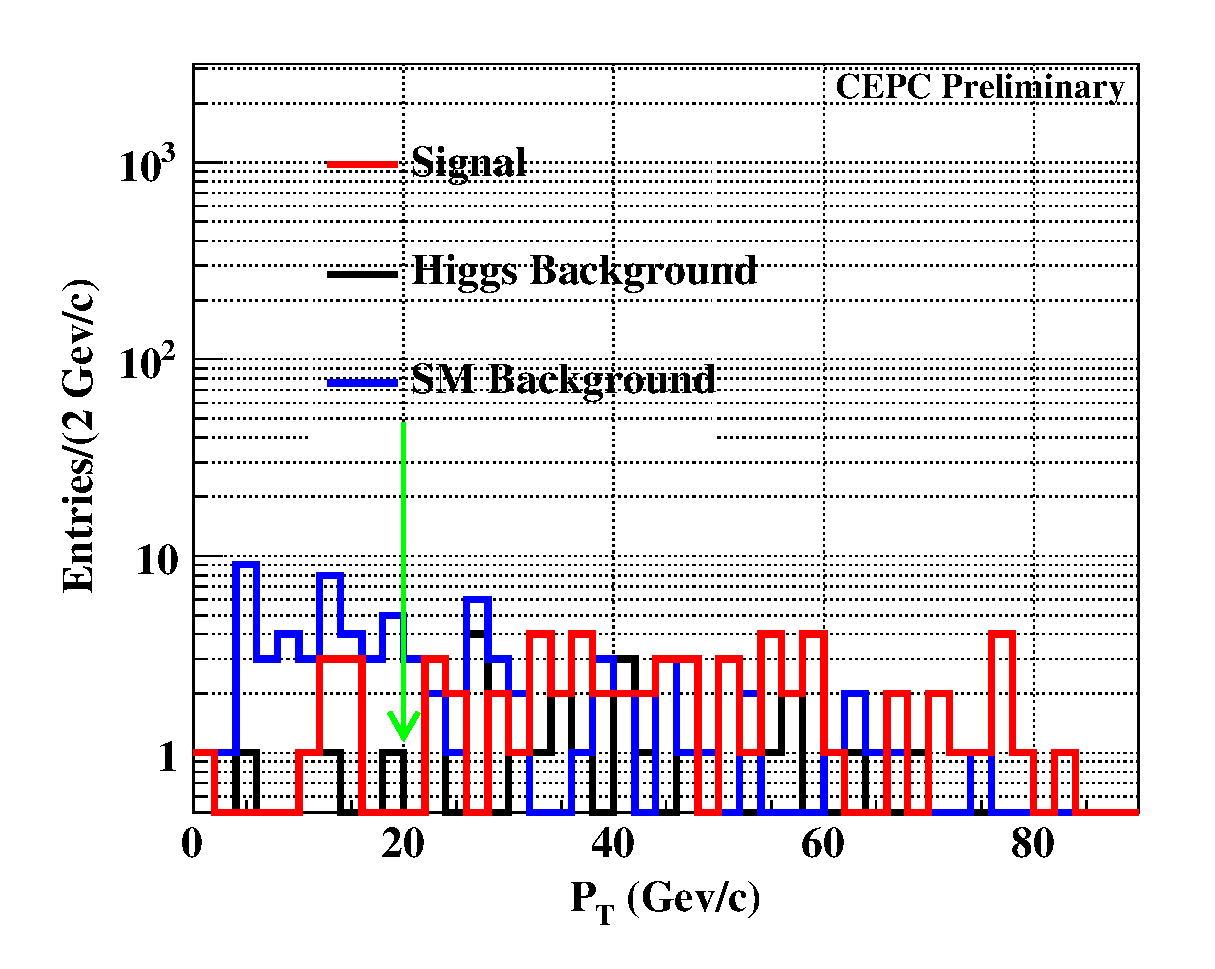
\includegraphics[width=0.5\textwidth]{e1e1H/evuv/ptineeevuv}
	\caption[]{The distribution of transverse momentum}
	\label{fig:ptineeevuv}
\end{figure}
The event selection is showed in Table~\ref{tab:eucutchain}.
\begin{table}[H]
  \begin{center}
    \begin{tabular}{cccc}
      \hline \hline
      \multicolumn{1}{c}{Category}&\multicolumn{1}{c}{Signal}&\multicolumn{1}{c}{$ZH$ background}&\multicolumn{1}{c}{SM background}\\ 
      \hline
      Total		       	 									&  192	& 37094	& 1303843\\
	  Validation of Pre-selection							&  104	& 21983	& 151498\\
      $N_{ZPole}=2; N_{Isolep}=2; l_1 = e, l_2 = \mu$	 	&  80	& 111	& 245\\
	  $N_{Remain} < 5$										&  80	& 88	& 208\\
	  $10\gev/c^2 < M_{Inv}^{e\mu} < 65\gev/c^2$	       	&  76	& 73	& 169	\\
	  $20\gev/c^2 < M_{Missing} < 70\gev/c^2$	        	&  65	& 28	& 70		\\
	  $P_{T} > 20\gev/c$									&  57	& 23	& 34		\\
	  $\sqrt{(\frac{D0}{sigD0})^2+(\frac{Z0}{sigZ0})^2} < 4$&  53 	& 3		& 3	\\
      \hline \hline
    \end{tabular}
   \caption[Monte Carlo purities in the single lepton sample]{Cut chain of $ee e\mu$ final state}
  \label{tab:eucutchain}
 \end{center}
\end{table}

Since the number of background after event selection is lower than 10, the detail of contained background would not be listed. 
According to Table~\ref{tab:eucutchain}, the events of signal are $N_{sig} = 53\pm 8$ by counting, and efficiency of signal 
selection is 27.6\%. The precision of this subchannel is 
\begin{equation*}
	Accu. = \frac{\sqrt{S+B}}{S} = 15.1\%.
\end{equation*}

\subsection{Analysis of $e^+e^- \to ZH, Z \to e^+e^-, H\to WW^* \to \mu\nu \mu\nu$ decay}
In this channel, the main background is also $eeZ$ process, and $Z$ boson decay to a pair of $\mu$. 
For the same reason mentioned before, transverse momentum of four leptons is applied.
\begin{figure}[H]
	\centering
	\includegraphics[width=0.5\textwidth]{e1e1H/uvuv/ptineeuvuv}
	\caption[]{The distribution of transverse momentum}
	\label{fig:ptineeuvuv}
\end{figure}
Events of $eeZ$ process would be reduced a lot after $p_T$ selection, as shown in Figure~\ref{fig:ptineeuvuv}. 
The cut chain is showed in Table~\ref{tab:cutchaineeuvuv}.
\begin{table}[H]
  \begin{center}
    \begin{tabular}{cccc}
      \hline \hline
      \multicolumn{1}{c}{Category}&\multicolumn{1}{c}{Signal}&\multicolumn{1}{c}{$ZH$ background}&\multicolumn{1}{c}{SM background}\\ 
      \hline
      Total		       	 									&  102	& 37094	& 1303843\\
	  Validation of Pre-selection							&  58	& 21983	& 151498\\
      $N_{ZPole}=2; N_{Isolep}=2; l_1 = \mu, l_2 = \mu$	 	&  57	& 92	& 4385\\
	  $N_{Remain} < 4$										&  57	& 50	& 4098\\
	  $5\gev/c^2 < M_{Inv}^{\mu\mu} < 60\gev/c^2$	   	   	&  53	& 41	& 1601	\\
	  $20\gev/c^2 < M_{Missing} < 65\gev/c^2$	        	&  46	& 3		& 320		\\
	  $P_{T} > 20\gev/c$									&  44	& 2		& 23		\\
	  $\sqrt{(\frac{D0}{sigD0})^2+(\frac{Z0}{sigZ0})^2} < 4$&  44 	& 1		& 17	\\
      \hline \hline
    \end{tabular}
   \caption[Monte Carlo purities in the single lepton sample]{Cut chain of $ee \mu\mu$ final state}
  \label{tab:cutchaineeuvuv}
 \end{center}
\end{table}

After event selection, the main background and its number are shown in Table~\ref{tab:bkgineeuvuv}.
\begin{table}[H]
	\begin{center}
		\begin{tabular}{lrc}
			\hline\hline
			Decay Chain	& Final States 	&	Number of Events	\\
			\hline
			$e^+e^-\to eeZ \to ee\mu\mu $ & $2e, 2\mu$	&	17\\
			\hline\hline
		\end{tabular}
		\caption[]{The main background and its number after event selection}
		\label{tab:bkgineeuvuv}
	\end{center}
\end{table}

Through counting, the events of signal is $N_{sig} = 44\pm 8$, and the efficiency of signal selection is 43.1\%.
The precision of this channel is:
\begin{equation*}
	Accu. = \frac{\sqrt{S+B}}{S} = 18.2\%.
\end{equation*}

\subsection{Analysis of $e^+e^- \to ZH, Z \to \mu^+\mu^-, H\to WW^* \to e\nu e\nu$ decay}
Since the final states in this channel are the same as $e^+e^- \to ZH, Z \to e^+e^-, H\to WW^* \to \mu\nu \mu\nu$ decay channel, 
it's no doubt that their main background are the same, $eeZ$ process. 
And transverse momentum of four leptons are also powerful to ruduce this background, as shown in Figure~\ref{fig:ptinuuevev}.
\begin{figure}[H]
	\centering
	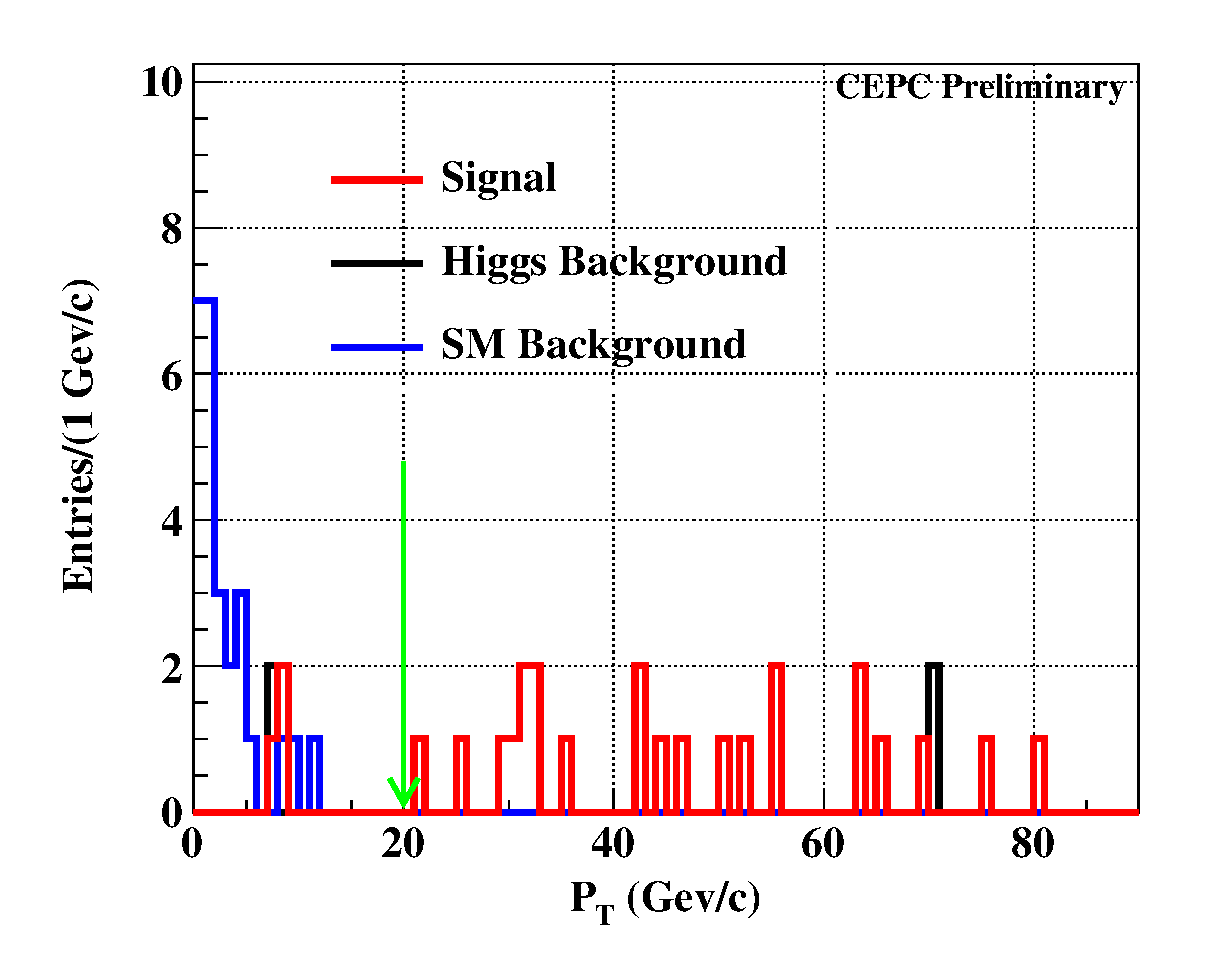
\includegraphics[width=0.5\textwidth]{e2e2H/evev/ptinuuevev}
	\caption[]{The distribution of transverse momentum}
	\label{fig:ptinuuevev}
\end{figure}

The detail of cut chain is shown in Table~\ref{tab:cutchainuuevev}.
\begin{table}[H]
  \begin{center}
    \begin{tabular}{cccc}
      \hline \hline
      \multicolumn{1}{c}{Category}&\multicolumn{1}{c}{Signal}&\multicolumn{1}{c}{$ZH$ background}&\multicolumn{1}{c}{SM background}\\ 
      \hline
      Total		       	 									&  89	& 35333	& 700311\\
	  Validation of Pre-selection							&  73	& 29479	& 117395\\
      $N_{ZPole}=2; N_{Isolep}=2; l_1 = e, l_2 = e$		 	&  48	& 117	& 5964	\\
	  $N_{Remain} < 4$										&  48	& 73	& 4968	\\
	  $5\gev/c^2 < M_{Inv}^{ee} < 45\gev/c^2$			   	&  39	& 48	& 204	\\
	  $20\gev/c^2 < M_{Missing} < 65\gev/c^2$	        	&  30	& 5		& 48	\\
	  $\sqrt{(\frac{D0}{sigD0})^2+(\frac{Z0}{sigZ0})^2} < 4$&  26 	& 2		& 26	\\
	  $P_{T} > 20\gev/c$									&  23	& 2		& 0		\\
      \hline \hline
    \end{tabular}
   \caption[Monte Carlo purities in the single lepton sample]{Cut chain of $\mu\mu ee$ final state}
  \label{tab:cutchainuuevev}
 \end{center}
\end{table}

Because the number of background is less than 10, the its detail would not be listed.
According to Table~\ref{tab:cutchainuuevev} and through counting, the number of signal events is $N_{sig} = 23\pm 5$. 
Efficiency of signal selection is 25.8\%. The precision of this channel is:
\begin{equation*}
	Accu. = \frac{\sqrt{S+B}}{S} = 21.7\%
\end{equation*}

\subsection{Analysis of $e^+e^- \to ZH, Z \to \mu^+\mu^-, H\to WW^* \to \mu\nu \mu\nu$ decay}
There are four muons as the visible final state in this channel, therefore the $ZZ$ process is the main background. 
Definitely, transverse momentum of four leptons is also useful to reduce this background, as shown in Figure~\ref{fig:ptinuuuvuv}.
\begin{figure}[H]
	\centering
	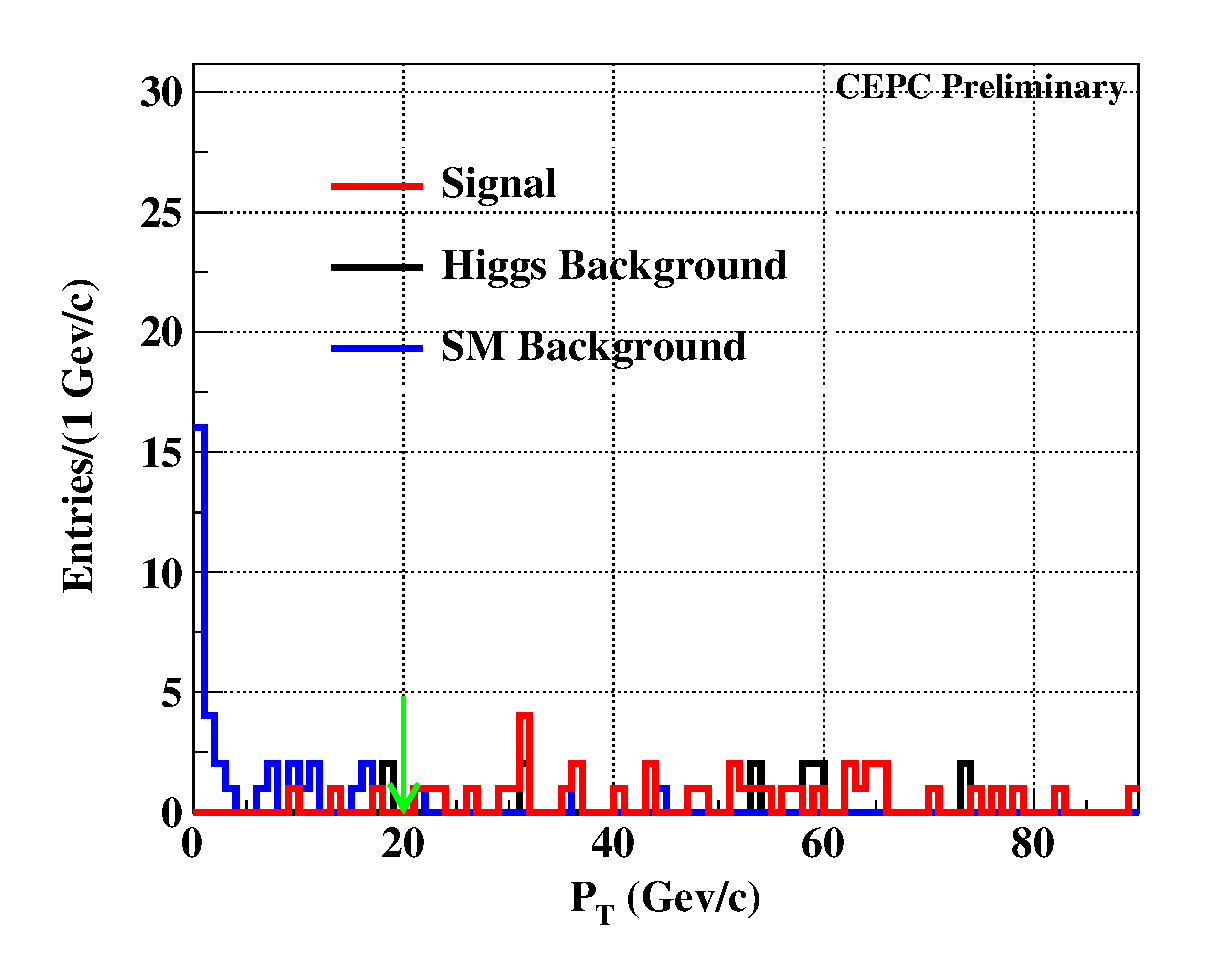
\includegraphics[width=0.5\textwidth]{e2e2H/uvuv/ptinuuuvuv}
	\caption[]{The distribution of transverse momentum}
	\label{fig:ptinuuuvuv}
\end{figure}
After the event selection, the cut chain is shown in Table~\ref{tab:cutchainuuuvuv}.
\begin{table}[H]
  \begin{center}
    \begin{tabular}{cccc}
      \hline \hline
      \multicolumn{1}{c}{Category}&\multicolumn{1}{c}{Signal}&\multicolumn{1}{c}{$ZH$ background}&\multicolumn{1}{c}{SM background}\\ 
      \hline
      Total		       	 									&  87	& 35333	& 700311\\
	  Validation of Pre-selection							&  68	& 29479	& 117395\\
      $N_{ZPole}=2; N_{Isolep}=2; l_1 = \mu, l_2 = \mu$		&  66	& 133	& 2661	\\
	  $N_{Remain} < 4$										&  63	& 71	& 2282	\\
	  $5\gev/c^2 < M_{Inv}^{\mu\mu} < 45\gev/c^2$		   	&  53	& 55	& 375	\\
	  $20\gev/c^2 < M_{Missing} < 65\gev/c^2$	        	&  43	& 12	& 63	\\
	  $\sqrt{(\frac{D0}{sigD0})^2+(\frac{Z0}{sigZ0})^2} < 4$&  42 	& 6		& 39	\\
	  $P_{T} > 20\gev/c$									&  39	& 5		& 4		\\
      \hline \hline
    \end{tabular}
   \caption[Monte Carlo purities in the single lepton sample]{Cut chain of $\mu\mu\mu\mu$ final state}
  \label{tab:cutchainuuuvuv}
 \end{center}
\end{table}

Because the number of background is less than 10, the its detail would not be listed.
According to Table~\ref{tab:cutchainuuuvuv} and through counting, the number of signal events is $N_{sig} = 39\pm 7$. 
Efficiency of signal selection is 44.8\%. The precision of this channel is:
\begin{equation*}
	Accu. = \frac{\sqrt{S+B}}{S} = 17.9\%
\end{equation*}

\section{Analysis of the other semi-leptonic decay}
In semi-leptonic decay channel, $eeH \to e\nu qq$, $\mu\mu H \to e\nu qq$ and $\mu\mu H \to \mu\nu qq$, these three channels are 
highly similar with $eeH \to \mu\nu qq$ channel, and the same variables have been applied in these three channel. 
Therefore, only the cut chain would be listed below, as well as the main background and its number of events.
For $\nu\nu H \to \nu\nu e\nu qq$ and $\nu\nu H \to \nu\nu \mu\nu qq$, they would be much different with the others
due to the initial $Z$ boson decay to two neotrinoes and there are only three visible pfos in the final states, 
so one of them would be introduced completely.
\subsection{Analysis of $e^+e^-\rightarrow ZH, Z\rightarrow e^+e^-, H\rightarrow WW^*, WW^*\rightarrow e\nu q\bar{q}$ decay}
Table~\ref{tab:cutchaineeevqq} shows the details of event selection, and Table~\ref{tab:bkgineeevqq} lists the main background in 
this channel.
\begin{table}[H]
  \begin{center}
    \begin{tabular}{cccc}
      \hline \hline
      \multicolumn{1}{c}{Category}&\multicolumn{1}{c}{Signal}&\multicolumn{1}{c}{$ZH$ background}&\multicolumn{1}{c}{SM background}\\ 
      \hline
      Total 	      	 									&   1177	& 35142	& 1303847\\
      $N_{ZPole}=2; N_{Isolep}=1; N_{Jets} =2; l = e$		&   882		& 1235	& 64595\\
	  Validation of Pre-selection							&	598		& 693	& 8437		\\
	  $7 < N_{Remain} < 30$									&	567		& 208	& 961\\
	  $10\gev/c^2 < M_{Inv}^{di-Jet} < 95\gev/c^2 $			&	542		& 136	& 662\\
	  $Btag < 0.9$											&	535		& 102	& 428\\
	  $M_{Missing} < 45\gev/c^2$							&   523		&  50	& 393\\
	  $\sqrt{(\frac{D0}{sigD0})^2+(\frac{Z0}{sigZ0})^2} < 9$&   490   	&  23 	& 278\\
	  $p_T > 10 \gev/c$										&	435		&  13	& 61\\
      \hline \hline
    \end{tabular}
  \caption[Monte Carlo purities in the single lepton sample]{% Monte
    Cut chain of semi leptonic decay of $ZH\rightarrow ZWW^* \rightarrow eee\nu qq$}
  \label{tab:cutchaineeevqq}
  \end{center}
\end{table}

\begin{table}[H]
	\begin{center}
		\begin{tabular}{lrc}
			\hline\hline
			Decay Chain	& Final States 	&	Number of Events	\\
			\hline
			$e^+e^-\to eeZ \to ee\tau\tau $ & $2e, 2\tau$	&	11\\
			$e^+e^-\to eeZ \to eeqq $ 		& $2e, 2q$		&	46\\
			\hline\hline
		\end{tabular}
		\caption[]{The main background and its number after event selection}
		\label{tab:bkgineeevqq}
	\end{center}
\end{table}
There are some $\tau$ events in the background, and it could be reduced by a reliable $\tau-$finding. 
Although the number of $ZH$ background events is larger than 10, it includes more than two parts, such as $ZH \to \nu\nu\tau\nu qq$
and $ZH \to b\bar{b}$. Therefore, the detail of $ZH$ background would not be listed.
According to this result, the number of signal events is $N_{sig} = 435\pm 23$. Efficiency of signal selection is 37.0\%. 
The precision is:
\begin{equation*}
	Accu. = \frac{\sqrt{S+B}}{S} = 5.3\%.
\end{equation*}

\subsection{Analysis of $e^+e^-\rightarrow ZH, Z\rightarrow \mu^+\mu^-, H\rightarrow WW^*, WW^*\rightarrow e\nu q\bar{q}$ decay}
Table~\ref{tab:cutchainuuevqq} shows the details of event selection, and Table~\ref{tab:bkginuuevqq} lists the main background in 
this channel.
\begin{table}[H]
  \begin{center}
    \begin{tabular}{cccc}
      \hline \hline
      \multicolumn{1}{c}{Category}&\multicolumn{1}{c}{Signal}&\multicolumn{1}{c}{$ZH$ background}&\multicolumn{1}{c}{SM background}\\ 
      \hline
      Total 	      	 									&   1108	& 33207	& 1303847\\
      $N_{ZPole}=2; N_{Isolep}=1; N_{Jets} =2; l = e$		&   842		& 961	& 23524\\
	  Validation of Pre-selection							&	739		& 789	& 3167	\\
	  $7 < N_{Remain} < 30$									&	704		& 220	& 213\\
	  $10\gev/c^2 < M_{Inv}^{di-Jet} < 95\gev/c^2 $			&	688		& 160	& 137\\
	  $Btag < 0.9$											&	683		& 120	& 83\\
	  $M_{Missing} < 45\gev/c^2$							&   675		&  73	& 74\\
	  $\sqrt{(\frac{D0}{sigD0})^2+(\frac{Z0}{sigZ0})^2} < 4$&   580   	&  25 	& 21\\
	  $p_T > 4 \gev/c$										&	573		&  22	& 8\\
      \hline \hline
    \end{tabular}
  \caption[Monte Carlo purities in the single lepton sample]{% Monte
    Cut chain of semi leptonic decay of $ZH\rightarrow ZWW^* \rightarrow \mu\mu e\nu qq$}
  \label{tab:cutchainuuevqq}
  \end{center}
\end{table}

\begin{table}[H]
	\begin{center}
		\begin{tabular}{lrc}
			\hline\hline
			Decay Chain	& Final States 	&	Number of Events	\\
			\hline
			$e^+e^-\to ZH \to ZWW^* \to \mu\mu\tau\nu qq $ 		& $2\mu, \tau, \nu, 2q$		&	21\\
			\hline\hline
		\end{tabular}
		\caption[]{The main background and its number after event selection}
		\label{tab:bkginuuevqq}
	\end{center}
\end{table}
In this channel, the main background is $ZH \to \mu\mu\tau\nu qq$ decay channel, and $\tau$ decay to a electron. 
As we all known, energy of electron which come from $\tau$ is much more lower than its from signal. 
Because of the few number of background, it's not useful to distinguish them. 
According to this result, the number of signal events is $N_{sig} = 573\pm 25$. Efficiency of signal selection is 51.7\%. 
The precision is:
\begin{equation*}
	Accu. = \frac{\sqrt{S+B}}{S} = 4.4\%.
\end{equation*}

\subsection{Analysis of $e^+e^-\rightarrow ZH, Z\rightarrow \mu^+\mu^-, H\rightarrow WW^*, WW^*\rightarrow \mu\nu q\bar{q}$ decay}
Table~\ref{tab:cutchainuuuvqq} shows the details of event selection, and Table~\ref{tab:bkginuuuvqq} lists the main background in 
this channel.
\begin{table}[H]
  \begin{center}
    \begin{tabular}{cccc}
      \hline \hline
      \multicolumn{1}{c}{Category}&\multicolumn{1}{c}{Signal}&\multicolumn{1}{c}{$ZH$ background}&\multicolumn{1}{c}{SM background}\\ 
      \hline
      Total 	      	 									&   1105	& 33207	& 1303847\\
      $N_{ZPole}=2; N_{Isolep}=1; N_{Jets} =2; l = \mu$		&   970		& 1756	& 11007\\
	  Validation of Pre-selection							&	849		& 1494	& 1893\\
	  $7 < N_{Remain} < 30$									&	807		& 664	& 723	\\
	  $10\gev/c^2 < M_{Inv}^{di-Jet} < 95\gev/c^2 $			&	794		& 353	& 588	\\
	  $Btag < 0.9$											&	787		& 149	& 238	\\
	  $M_{Missing} < 45\gev/c^2$							&   778		&  89	& 226	\\
	  $\sqrt{(\frac{D0}{sigD0})^2+(\frac{Z0}{sigZ0})^2} < 4$&   772   	&  32 	& 184	\\
	  $p_T > 4 \gev/c$										&	756		&  30	& 123	\\
      \hline \hline
    \end{tabular}
  \caption[Monte Carlo purities in the single lepton sample]{% Monte
    Cut chain of semi leptonic decay of $ZH\rightarrow ZWW^* \rightarrow\mu\mu\mu\nu qq$}
  \label{tab:cutchainuuuvqq}
  \end{center}
\end{table}

\begin{table}[H]
	\begin{center}
		\begin{tabular}{lrc}
			\hline\hline
			Decay Chain	& Final States 	&	Number of Events	\\
			\hline
			$e^+e^-\to ZH \to ZWW^* \to \mu\mu\tau\nu qq $ 	& $2\mu, \tau, \nu, 2q$	&	22\\
			$e^+e^-\to ZZ \to \mu\mu qq $ 					& $2\mu, 2q$		&	117\\
			\hline\hline
		\end{tabular}
		\caption[]{The main background and its number after event selection}
		\label{tab:bkginuuuvqq}
	\end{center}
\end{table}
There are some $\tau$ events in the $ZH$ background, and it could be reduced by a reliable $\tau-$finding. 
According to this result, the number of signal events is $N_{sig} = 756\pm 30$. Efficiency of signal selection is 68.4\%. 
The precision is:
\begin{equation*}
	Accu. = \frac{\sqrt{S+B}}{S} = 4.0\%.
\end{equation*}

\subsection{Analysis of $e^+e^-\rightarrow ZH, Z\rightarrow \nu\nu, H\rightarrow WW^*, WW^*\rightarrow \mu\nu q\bar{q}$ decay}
Compared to the $\nu\nu qqqq$ channel, there are only three pfos in the final state. Therefore the conditions of pre-selection 
would be a little different after the number of pfos applied, 
shown in Table~\ref{tab:nnhuvqqprecut} and Figure~\ref{fig:nnHuvqqfiltered}.
\begin{figure}[H]
	\centering
	\subfigure[]{
		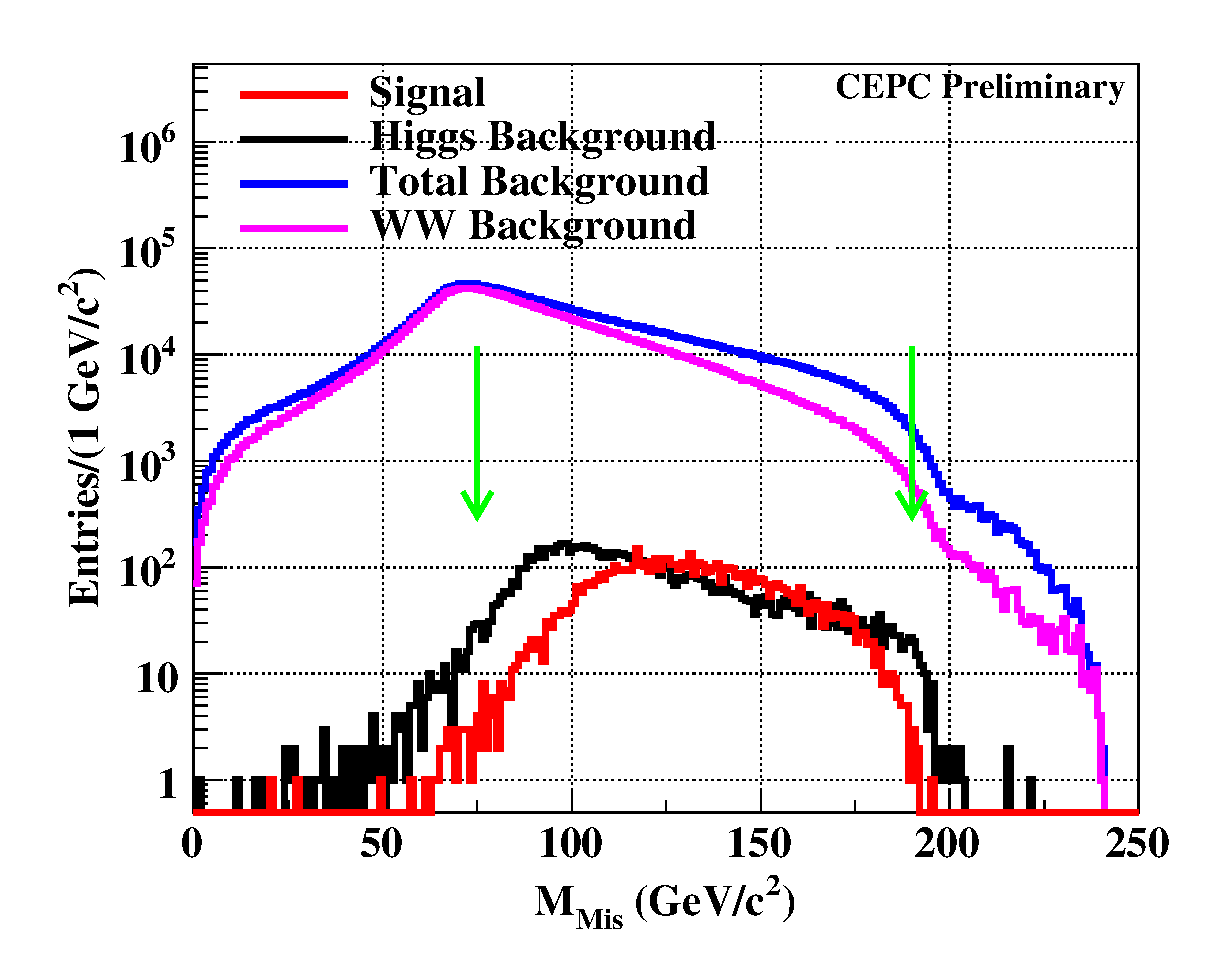
\includegraphics[width=0.35\textwidth]{nnH/lvqq/uvqq/MisMass}
	}
	\subfigure[]{
		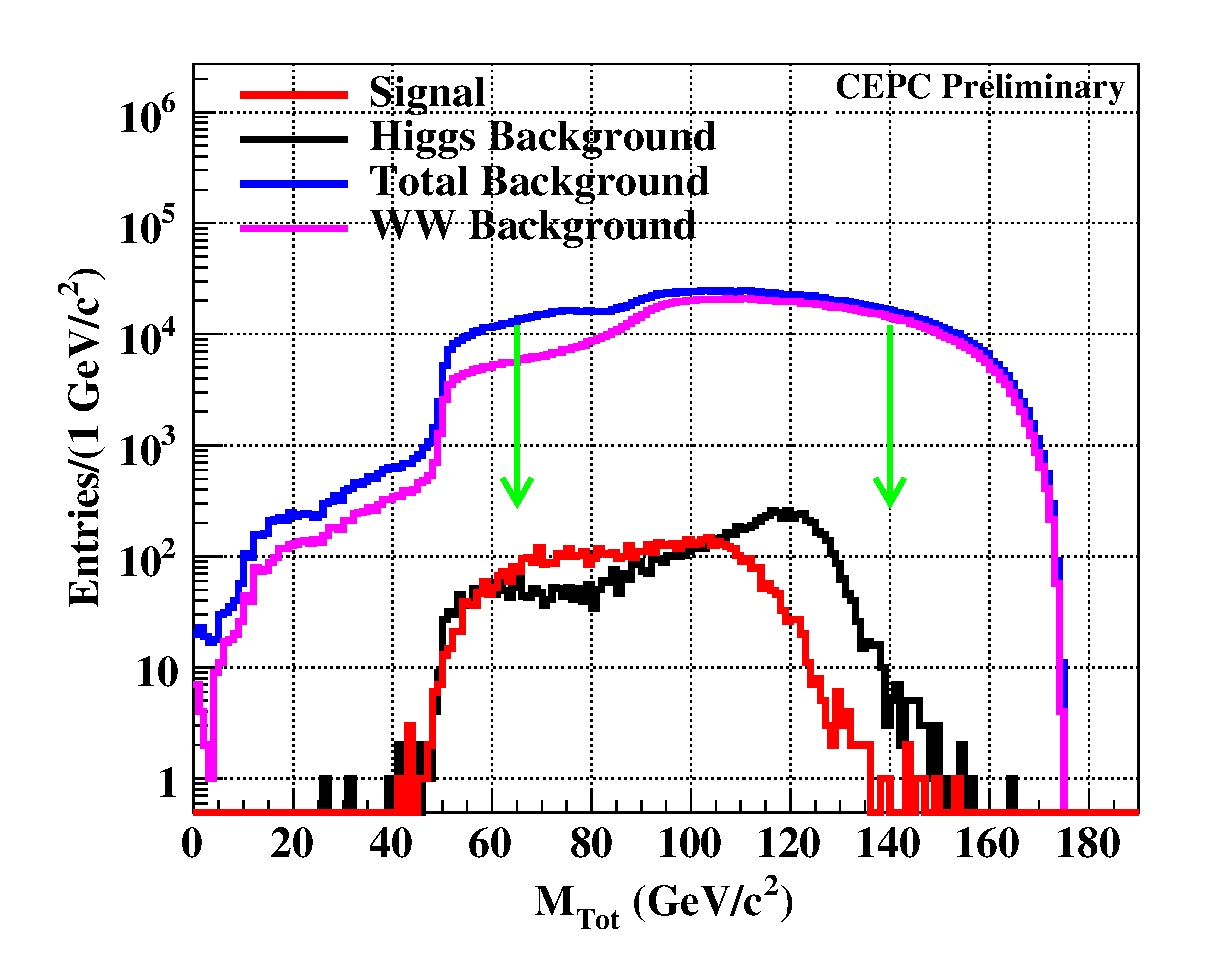
\includegraphics[width=0.35\textwidth]{nnH/lvqq/uvqq/VisMass}
	}
	\subfigure[]{
		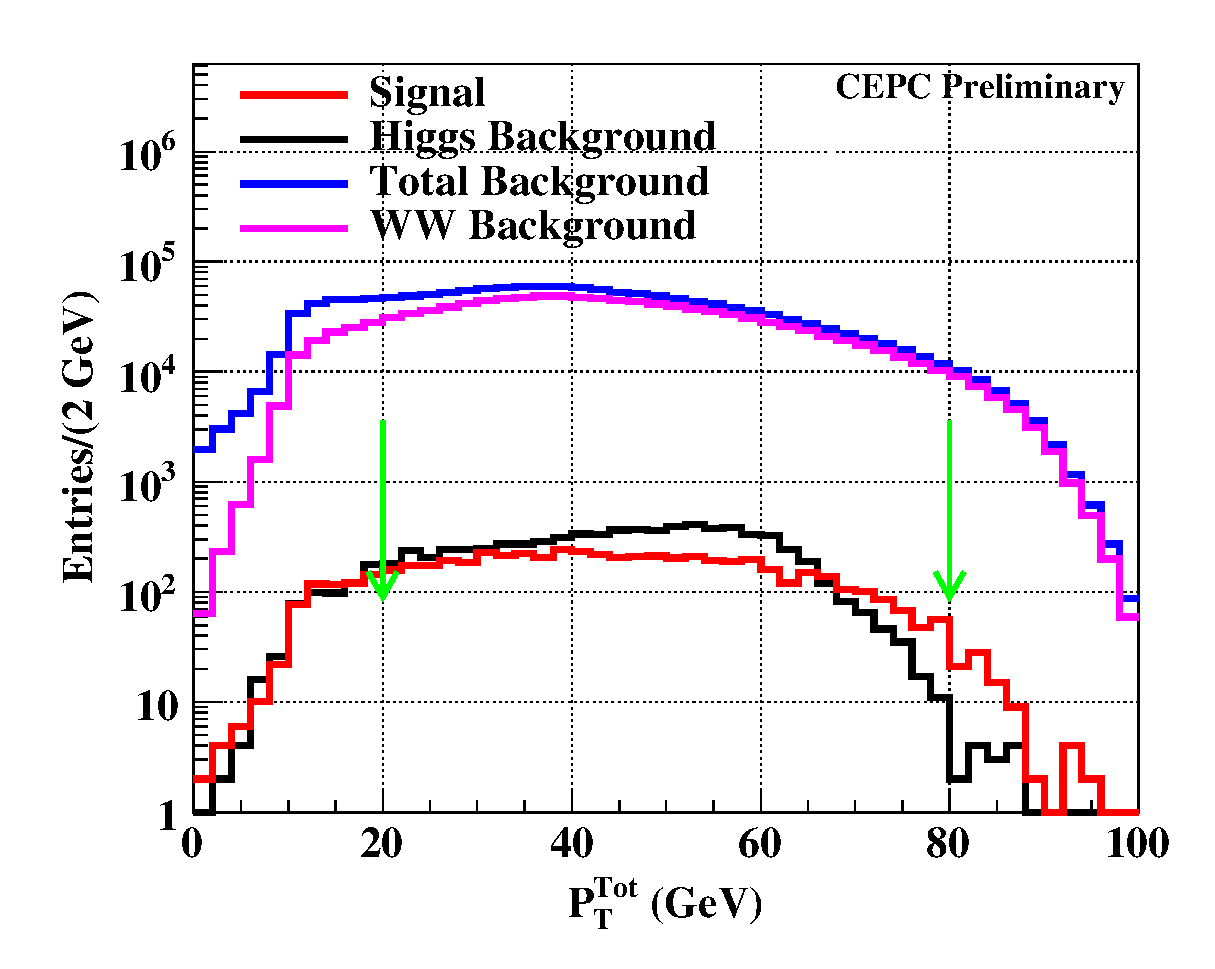
\includegraphics[width=0.35\textwidth]{nnH/lvqq/uvqq/TotalPt}
	}
	\caption[]{The distribution of missing mass, total mass and total transverse momentum in full simulation 
		in $\nu\nu\mu\nu qq$ channel. Compared to the $\nu\nu qqqq$ channel, upper missing mass should be lower, 
		and visible mass should be shifted left. Transverse momentum would be same.
		Top: The left is missing mass of event. The right is total mass of event.
		Bottom: It is the distribution of total transverse momentum of event.}
	\label{fig:nnHuvqqfiltered}
\end{figure}
\begin{table}[H]
  \begin{center}
  \begin{tabular}{|c|c|}
  \hline \hline
  Process of signal								&		$\nu\nu H \to \nu\nu \mu \nu qq$\\
  \hline
  \multirow{3}{*}{conditions of pre-selection}	&	$65\gev/c^2 < M_{Mis} < 225\gev/c^2$	\\
  												&	$M_{Tot} > 50\gev/c^2$\\
												&	$10\gev/c < p_{T} < 100\gev/c$	\\
  \hline
  \multirow{3}{*}{conditions of validation}		&	$75\gev/c^2 < M_{Mis} < 140\gev/c^2$	\\
  												&	$65\gev/c^2 < M_{Tot} < 140\gev/c^2$	\\
												&	$20\gev/c < p_{T} < 80\gev/c$	\\
  \hline \hline
  \end{tabular}
  \caption[]{Conditions of pre-selection in MC and validation in full simulation of $\nu\nu H \to \nu\nu \mu \nu qq$ process}
 \end{center}
  \label{tab:nnhuvqqprecut}
\end{table}

Since it is a semi-leptonic decay channel, the number of particles except for the isolated lepton, shown in 
Figure~\ref{fig:vvuvqqnRem} 
would be larger than pure leptonic decay channel and lower than pure hadronic decay channel. 

To reduce the events of $\tau$ and $b$ background, the vertex parameter is a useful condition by requiment of 
$\sqrt{(\frac{D_{0}}{sigD_{0}})^2+(\frac{Z_{0}}{sigZ_{0}})^2}$, shown in Figure~\ref{fig:vvuvqqVertex}. 
\begin{figure}[H]
	\centering
	\subfigure[]{
		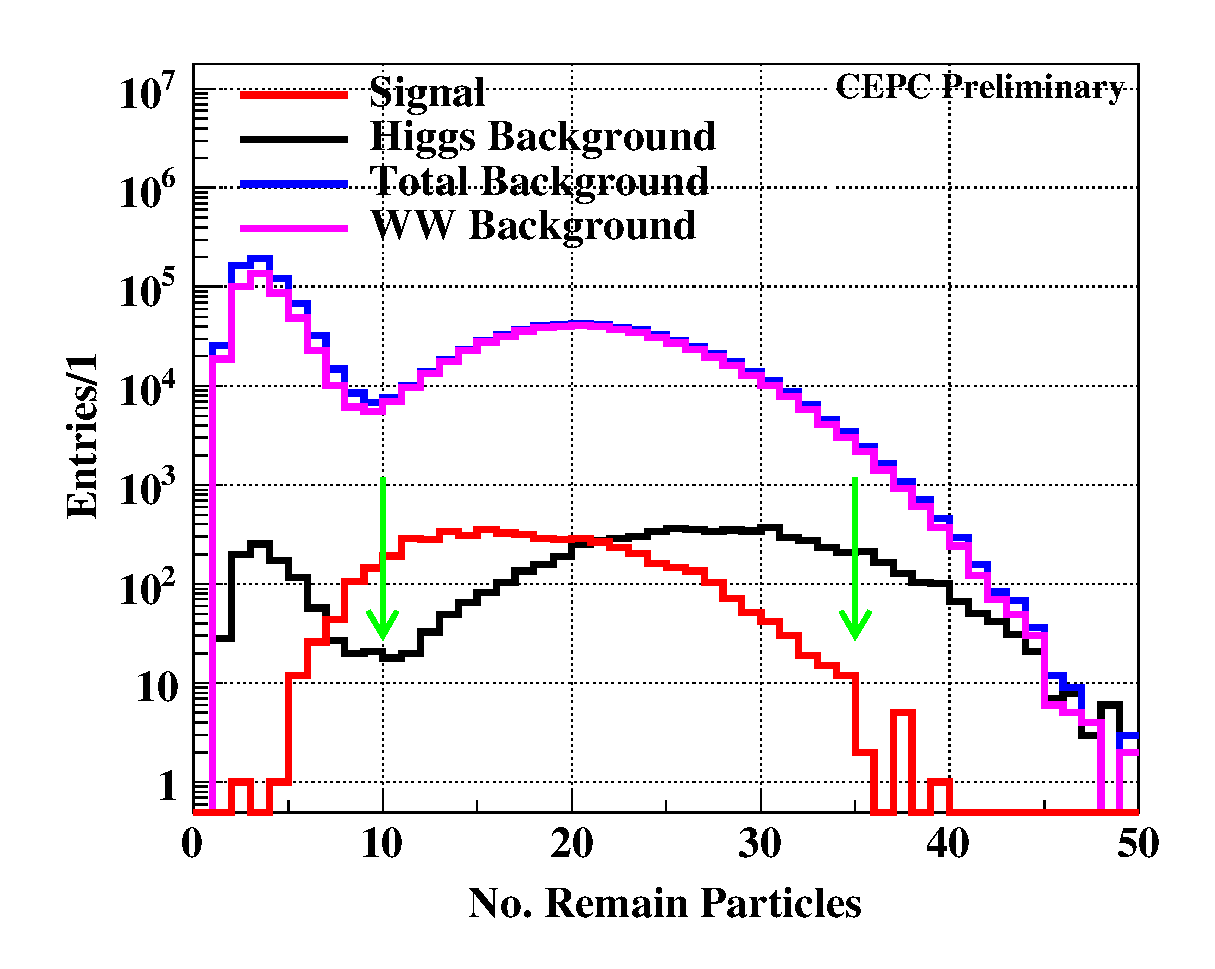
\includegraphics[width=0.35\textwidth]{nnH/lvqq/uvqq/nRem}
		\label{fig:vvuvqqnRem}
	}
	\subfigure[]{
		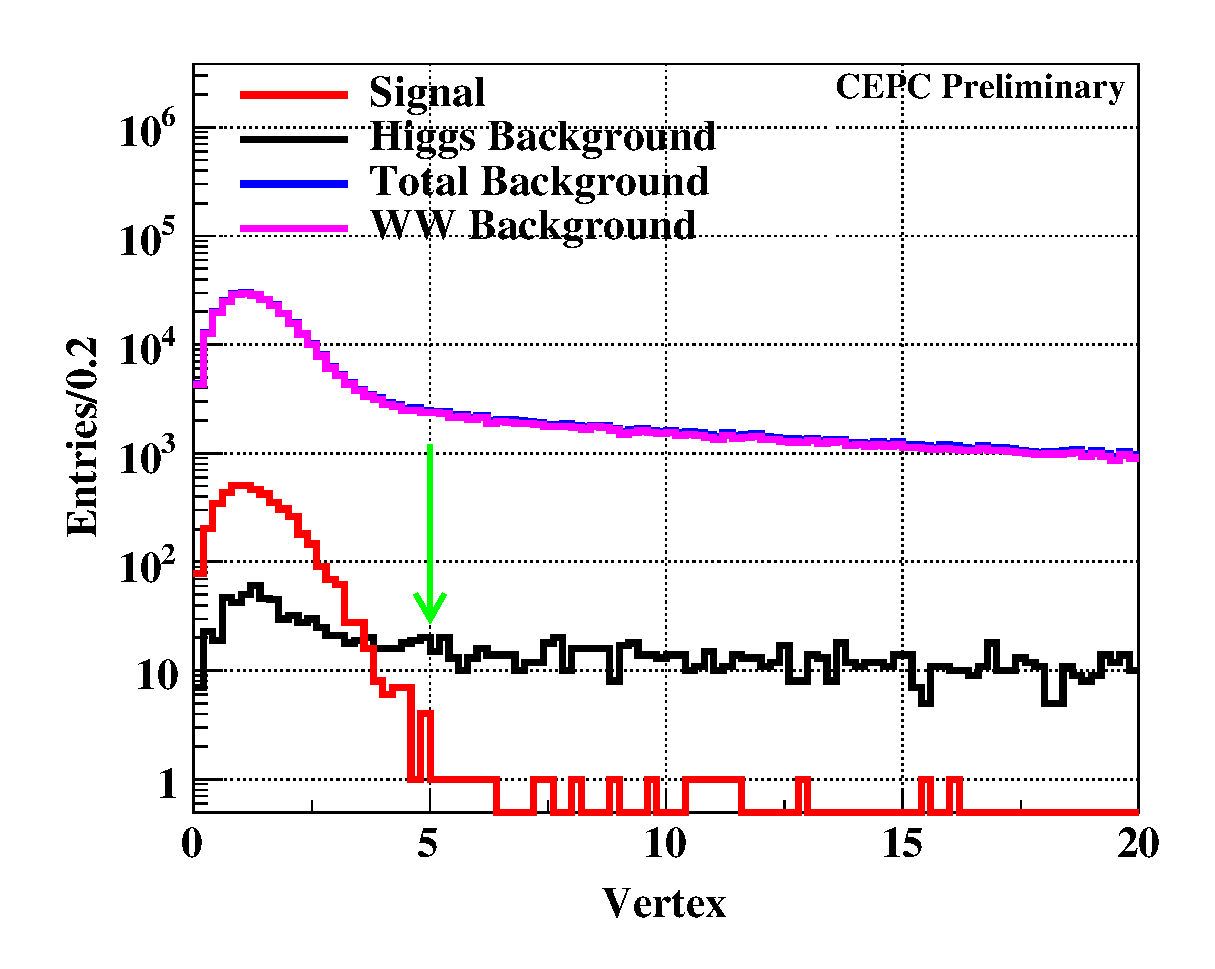
\includegraphics[width=0.35\textwidth]{nnH/lvqq/uvqq/LeptonVertex}
		\label{fig:vvuvqqVertex}
	}
	\caption[]{The distribution of particles number and the distance of $\mu$ and IP in $\nu\nu\mu\nu qq$ channel.
		}
	\label{fig:nnHuvqqremver}
\end{figure}
The main background is $WW$ channel right now. In order to reduce this background, a 2-dimensional distribution would be applied. 
As shown in Figure~\ref{fig:nnHuvqqEnerInvM}, the events in two regions, two black boxes in the plot, would be survived. 
\begin{figure}[H]
	\centering
	\subfigure[]{
		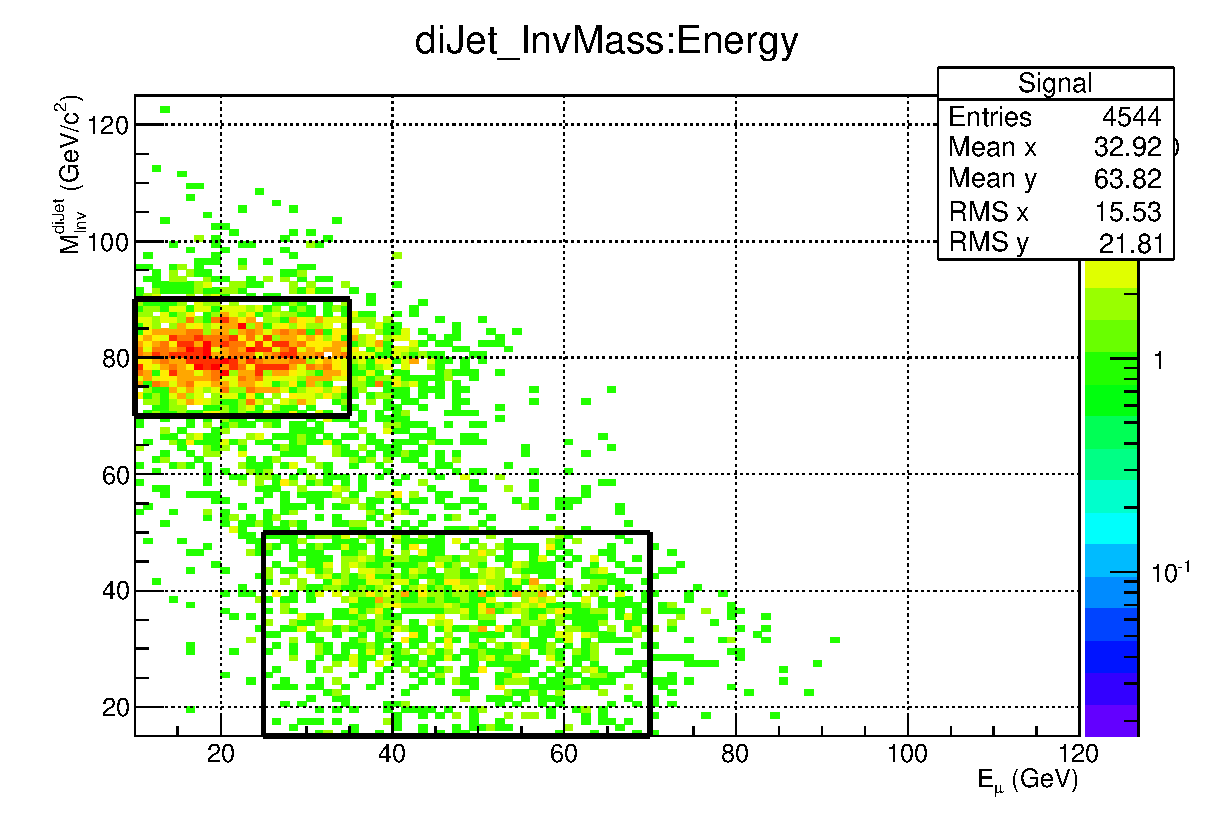
\includegraphics[width=0.35\textwidth]{nnH/lvqq/uvqq/TDsignal}
	}
	\subfigure[]{
		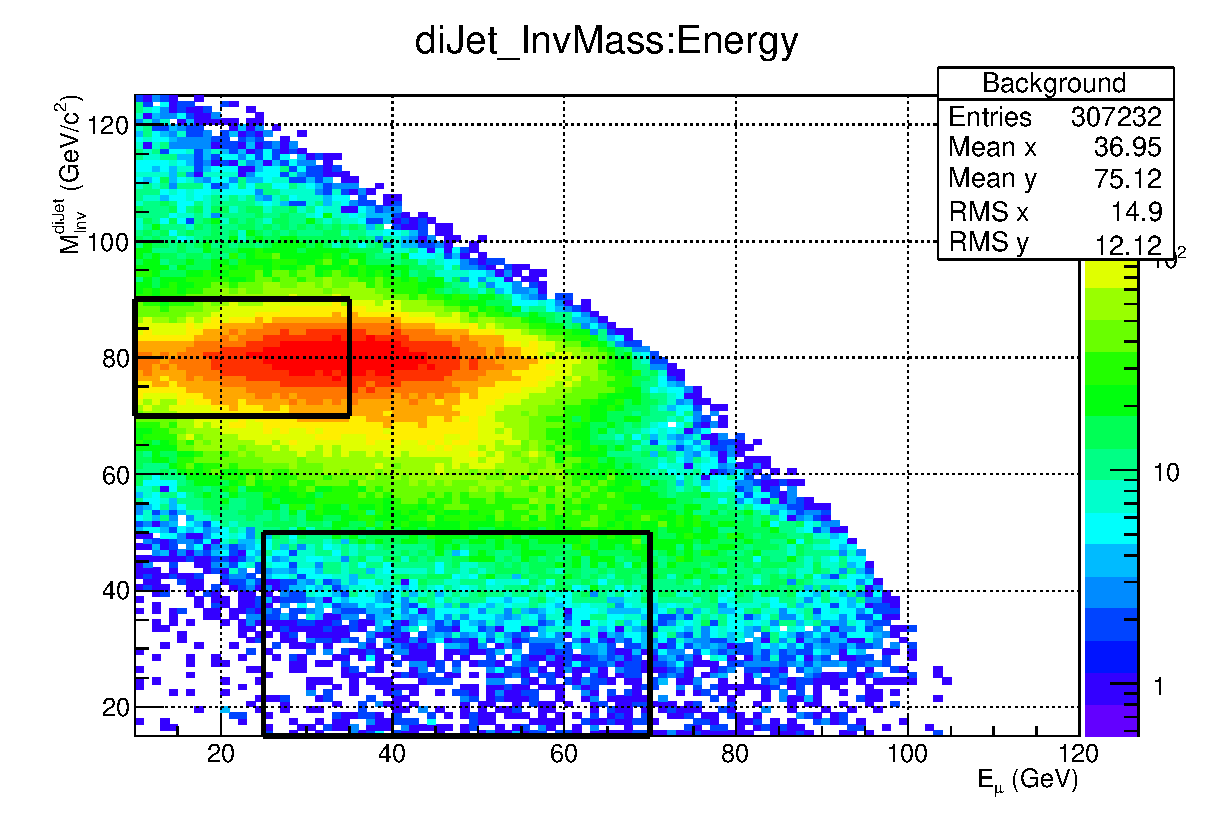
\includegraphics[width=0.35\textwidth]{nnH/lvqq/uvqq/TDbackground}
	}
	\caption[]{The distribution of lepton energy vs. di-jet invariant mass in $\nu\nu\mu\nu qq$ channel. 
		The left plot is the signal process and the right one is the background process which includes $ZH$ background and 
		SM background. X-axis is the energy of lepton and Y-axis is the invariant mass of di-jet.}
	\label{fig:nnHuvqqEnerInvM}
\end{figure}

Due to the main background is $WW$ background, the recoil mass of di-jet is another powerful condition to reduce, 
as shown in Figure~\ref{fig:nnHuvqqrecojet}. The recoil mass of some background events would be near to the $W$ mass.
\begin{figure}[H]
	\centering
	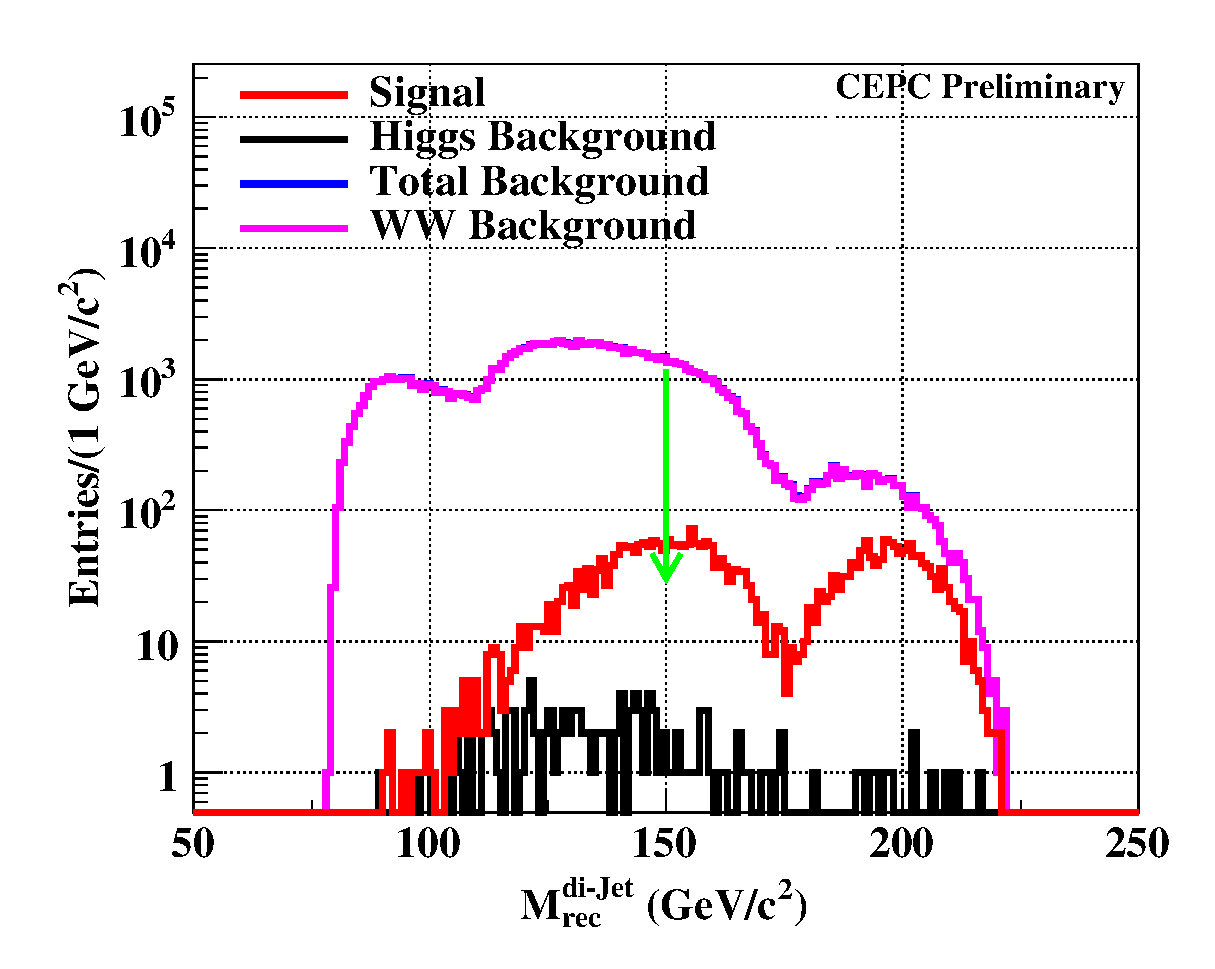
\includegraphics[width=0.5\textwidth]{nnH/lvqq/uvqq/JetReco}
	\caption[]{The distribution of recoil mass of di-jet.}
	\label{fig:nnHuvqqrecojet}
\end{figure}

Then, some variables would be put into TMVA for test and training, and the BDT(Boosted decision trees) method is applied.
The Figure~\ref{fig:nnHuvqqtmvacm} shows the correlation matrix of signal and events,
and the result of test and training samples is shown in Figure~\ref{fig:nnHuvqqbdt}.
The input variables would be introduced below:
\begin{itemize}
	\item WWAngle: This is the angle of $WW$ boson, one of the $W$ bosons is conbined by di-jet, and the other one is lepton.
	\item RecE: The energy of the isolated lepton.
	\item Area: Three vectors of 3-dimensional momentum, A, B and C, could be given by three pfos in the event.
		Vab is equal to A minus B. Vbc is equal to B minus C. Vca is equal to C minus A.
		And a triangle would be constructed by these three vectors, Vab, Vbc and Vca. The area is the area of this triangle.
	\item NorCosThe: It is the polar angle of area which is mentioned before. 
	\item Z0 and D0: They are the vertex parameter of lepton.
	\item diJet\_angle: This is the angle between di-jet.
	\item CtagOne: This is the probobility of $c$ quark tagging for the more energetic jet.
	\item TotalPt and VisMass: These two variables are introduced in the pre-selection.
\end{itemize}
\begin{figure}[H]
	\centering
	\subfigure[]{
		\includegraphics[width=0.35\textwidth]{nnH/lvqq/uvqq/CorrelationMatrixS}
	}
	\subfigure[]{
		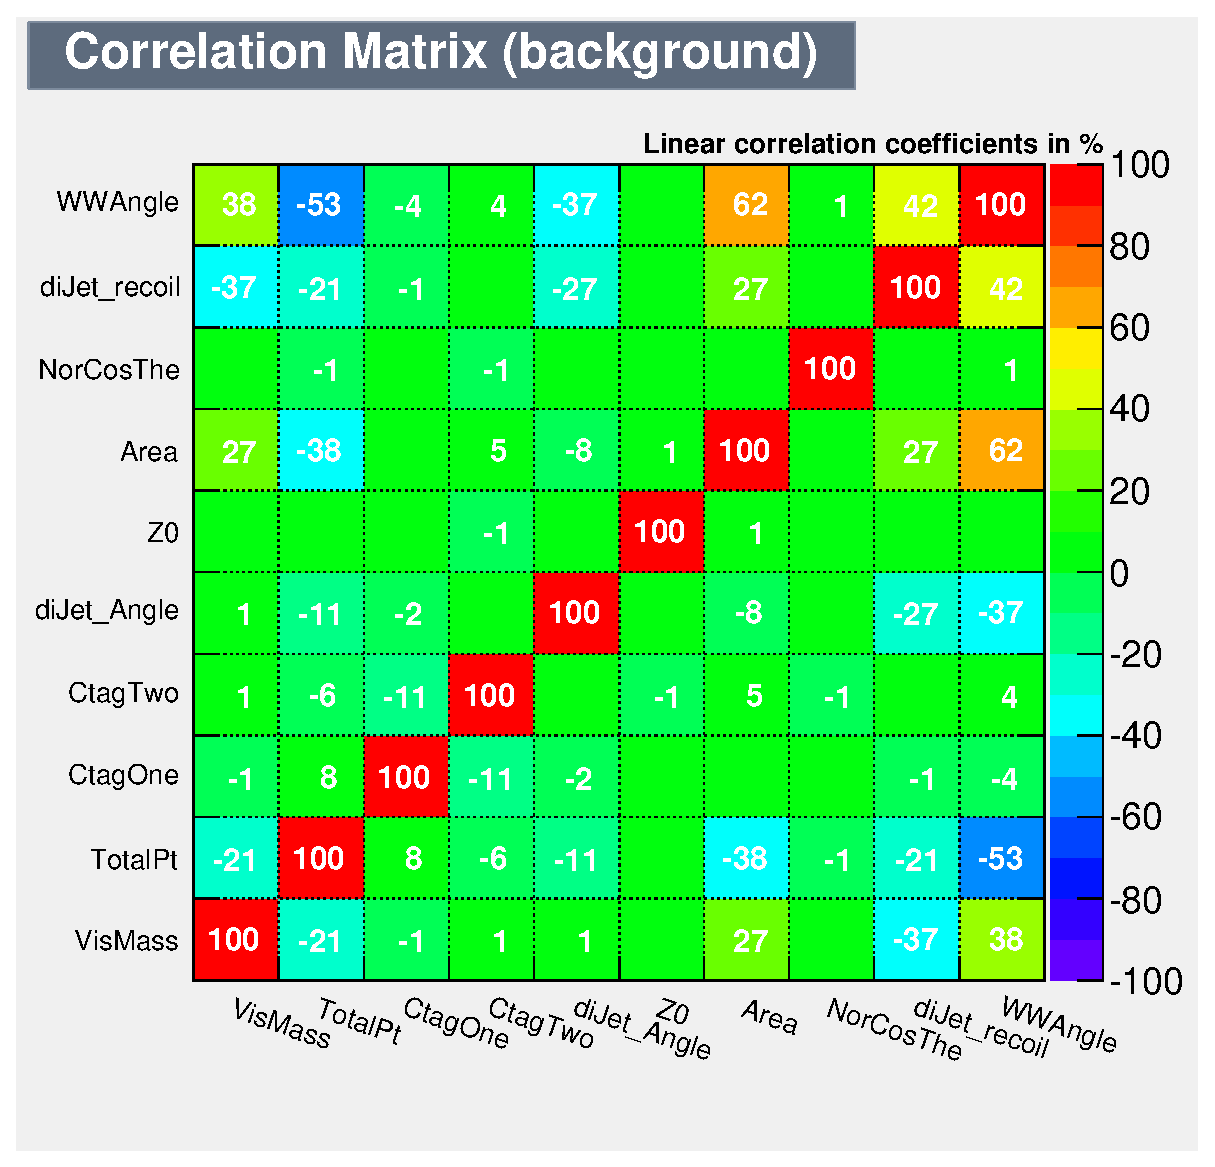
\includegraphics[width=0.35\textwidth]{nnH/lvqq/uvqq/CorrelationMatrixB}
	}
	\caption[]{The correlation matrix in $\nu\nu\mu\nu qq$ channel. 
		The left plot is the signal process and the right one is the background process which includes $ZH$ background and 
		SM background.}
	\label{fig:nnHuvqqtmvacm}
\end{figure}
\begin{figure}[H]
	\centering
	\includegraphics[width=0.5\textwidth]{nnH/lvqq/uvqq/overtrain_BDT}
	\caption[]{The result of BDT for test and training samples.}
	\label{fig:nnHuvqqbdt}
\end{figure}

After event selection, the detail of each step is shwon in Table~\ref{tab:cutchainvvuvqq} and the main background is listed in 
Table~\ref{tab:bkginvvuvqq}.
\begin{table}[H]
  \begin{center}
    \begin{tabular}{cccc}
      \hline \hline
      \multicolumn{1}{c}{Category}&\multicolumn{1}{c}{Signal}&\multicolumn{1}{c}{$ZH$ background}&\multicolumn{1}{c}{SM background}\\ 
      \hline
      Total 	      	 									&   7057	& 217161& 23469024	\\
	  $N_{ZPole}=2; N_{Isolep}=1; N_{Jets} =2; l = \mu$		&   6532	& 9006	& 3087607	\\
	  Validation of Pre-selection							&	5099	& 7291	& 1232771	\\
	  $10 < N_{Remain} < 35$								&	4564	& 5430	& 581219	\\
	  $\sqrt{(\frac{D0}{sigD0})^2+(\frac{Z0}{sigZ0})^2} < 5$&	4538	& 689	& 306543	\\
	  $E_{\mu} Vs. M_{Inv}^{di-jet}$						&	3322	& 131	& 113762	\\
	  $M_{Rec}^{di-jet} > 150\gev/c^2$						&   2200	& 39	& 24669		\\
	  $BDT >0.2$											&   790  	& 4 	& 315		\\
      \hline \hline
    \end{tabular}
  \caption[Monte Carlo purities in the single lepton sample]{% Monte
    Cut chain of semi leptonic decay of $ZH\rightarrow ZWW^* \rightarrow \nu\nu\mu\nu qq$}
  \label{tab:cutchainvvuvqq}
  \end{center}
\end{table}

\begin{table}[H]
	\begin{center}
		\begin{tabular}{lrc}
			\hline\hline
			Decay Chain	& Final States 	&	Number of Events	\\
			\hline
			$e^+e^-\to WW \to \tau\nu qq $ 	& $\tau, 2q$&	32\\
			$e^+e^-\to WW \to \mu\nu qq $ 	& $\mu, 2q$	&	274\\
			\hline\hline
		\end{tabular}
		\caption[]{The main background and its number after event selection}
		\label{tab:bkginvvuvqq}
	\end{center}
\end{table}
Through counting, the number of signal is $N_{sig} = 790\pm 33$, and the efficiency of signal selection is 11.2\%.
According to this result, the precision of this channel is:
\begin{equation*}
	Accu. =\frac{\sqrt{S+B}}{S} = 4.2\%.
\end{equation*}

\subsection{Analysis of $e^+e^-\rightarrow ZH, Z\rightarrow \nu\nu, H\rightarrow WW^*, WW^*\rightarrow e\nu q\bar{q}$ decay}
The process of this analysis is much similar with $\nu\nu\mu\nu qq$ channel, and the applied variables are also same. 
The same technique, BDT of TMVA, is also applied but the variables are little different with $\nu\nu\mu\nu qq$. 
The Figure~\ref{fig:nnHevqqtmvacm} shows the correlation matrix of signal and events,
and the result of test and training samples is shown in Figure~\ref{fig:nnHevqqbdt}.
The variables for BDT would be introduced below:
\begin{itemize}
	\item WWAngle: This is the angle of $WW$ boson, one of the $W$ bosons is conbined by di-jet, and the other one is lepton.
	\item diJet\_recoil: The recoil mass of di-jet.
	\item Area: Three vectors of 3-dimensional momentum, A, B and C, could be given by three pfos in the event.
		Vab is equal to A minus B. Vbc is equal to B minus C. Vca is equal to C minus A.
		And a triangle would be constructed by these three vectors, Vab, Vbc and Vca. The area is the area of this triangle.
	\item NorCosThe: It is the polar angle of area which is mentioned before. 
	\item Z0: It is the vertex parameter of lepton.
	\item diJet\_angle: This is the angle between di-jet.
	\item CtagOne and CtagTwo: They are the probobilitis of $c$ quark tagging for two jet.
	\item TotalPt and VisMass: These two variables are introduced in the pre-selection.
\end{itemize}
\begin{figure}[H]
	\centering
	\subfigure[]{
		\includegraphics[width=0.35\textwidth]{nnH/lvqq/evqq/CorrelationMatrixS}
	}
	\subfigure[]{
		\includegraphics[width=0.35\textwidth]{nnH/lvqq/evqq/CorrelationMatrixB}
	}
	\caption[]{The correlation matrix in $\nu\nu e\nu qq$ channel. 
		The left plot is the signal process and the right one is the background process which includes $ZH$ background and 
		SM background.}
	\label{fig:nnHevqqtmvacm}
\end{figure}
\begin{figure}[H]
	\centering
	\includegraphics[width=0.5\textwidth]{nnH/lvqq/evqq/overtrain_BDT}
	\caption[]{The result of BDT for test and training samples.}
	\label{fig:nnHevqqbdt}
\end{figure}
The detail of each step for event selection is shown in Table~\ref{tab:cutchainvvevqq}.
\begin{table}[H]
  \begin{center}
    \begin{tabular}{cccc}
      \hline \hline
      \multicolumn{1}{c}{Category}&\multicolumn{1}{c}{Signal}&\multicolumn{1}{c}{$ZH$ background}&\multicolumn{1}{c}{SM background}\\ 
      \hline
      Total 	      	 									&   6966	& 217252& 23469024	\\
	  $N_{ZPole}=2; N_{Isolep}=1; N_{Jets} =2; l = \mu$		&   5730	& 3495	& 3019180	\\
	  Validation of Pre-selection							&	4468	& 2388	& 1258539	\\
	  $10 < N_{Remain} < 35$								&	3971	& 1312	& 528845	\\
	  $\sqrt{(\frac{D0}{sigD0})^2+(\frac{Z0}{sigZ0})^2} < 5$&	3511	& 316	& 261404	\\
	  $E_{\mu} Vs. M_{Inv}^{di-jet}$						&	2587	& 63	& 93618		\\
	  $M_{Rec}^{di-jet} > 150\gev/c^2$						&   1764	& 31	& 20591		\\
	  $BDT >0.2$											&   680  	& 4 	& 359		\\
      \hline \hline
    \end{tabular}
  \caption[Monte Carlo purities in the single lepton sample]{% Monte
    Cut chain of semi leptonic decay of $ZH\rightarrow ZWW^* \rightarrow \nu\nu e\nu qq$}
  \label{tab:cutchainvvevqq}
  \end{center}
\end{table}
The below plot,Table~\ref{tab:bkginvvevqq}, is listed the main background which number of events are larger than 10.
\begin{table}[H]
	\begin{center}
		\begin{tabular}{lrc}
			\hline\hline
			Decay Chain	& Final States 	&	Number of Events	\\
			\hline
			$e^+e^-\to WW \to \tau\nu qq $ 	& $\tau, 2q$	&	13\\
			$e^+e^-\to e\nu W \to e\nu qq $ & $e, 2q$		&	344\\
			\hline\hline
		\end{tabular}
		\caption[]{The main background and its number after event selection}
		\label{tab:bkginvvevqq}
	\end{center}
\end{table}
Through counting, the number of signal is $N_{sig} = 680\pm 32$, and the efficiency of signal selection is 9.8\%.
According to this result, the precision of this channel is:
\begin{equation*}
	Accu. =\frac{\sqrt{S+B}}{S} = 4.7\%.
\end{equation*}


\section{Isolated leptons' condition}
\label{app:isolepcondition}
Isolated leptons tagging is a key in $WW^*$ analysis, especially in jets environment, so a good iaolated leptons algorithm
could decide our analysis accuracy. We will introduce the isolated leptons algorithm below:\\
There are two key conditions. The first one is lepton identification that a good PFA could help us.
The second is isolated conditions, cone angle of lepton and the ratio of energy in cone angle and lepton's energy, 
shown in Table~\ref{tab:isolep}.
\begin{table}[H]
\begin{center}
\begin{tabular}{cccccc}
\hline \hline
\multirow{2}{*}{$E_{lepton}$} & \multirow{2}{*}{Leptons' flavor} 	& \multicolumn{2}{c}{Full-leptonic Decay} 
& \multicolumn{2}{c}{Semi-leptonic Decay}\\
							&									&Cone Angle[rad]&$E_{Cone}/E_{Lepton}$
							&Cone Angle[rad]&$E_{Cone}/E_{Lepton}$\\
\hline
\multirow{2}{*}{$5\gev-10\gev$}	&			Muon					&0.15		&0.25		&0.15		&0.7	\\
							&			Electron				&0.3		&1.1		&0.3		&0.9	\\
\hline
\multirow{2}{*}{$10\gev-15\gev$}	&			Muon					&0.15		&0.35		&0.15		&0.25	\\
							&			Electron				&0.3		&0.75		&0.3		&0.75	\\
\hline
\multirow{2}{*}{$>15\gev$}	&			Muon					&0.15		&0.3		&0.15		&0.25	\\
							&			Electron				&0.25		&0.55		&0.25		&0.6	\\
\hline \hline
\end{tabular}
\caption{Isolated lepton condition}
\label{tab:isolep}
\end{center}
\end{table}
%\section{The {\tt cepcnote} class}
%\label{app:CepcNoteCls}
%
%This paper has been typeset using the {\tt cepcnote.cls} class, that
%implement the CEPC template can be used for papers, preprints,
%notes. The {\tt cepcnote} class is available on web pages of the
%Publication Committee, as well as this instruction paper and the
%related files.
%
%{\tt cepcnote.cls} derives from the standard \LaTeX{} {article.cls}
%class, thus all the usual commands and options you would have used
%with {\tt article} will work with it. For instance, this paper has
%been produced using this very simple preamble:
%
%\begin{verbatim}
%  \documentclass[11pt,a4paper]{cepcnote}
%  \graphicspath{{figures/}}
%  \usepackage{cepcphysics}
%  \usepackage{subfigure}
%\end{verbatim}
%
%\subsection{Dependencies}
%
%The {\tt cepcnote} class depends on these packages, which presence in
%your system is required:
%\begin{itemize}
%  \item {\tt graphicx}
%  \item {\tt mathptmx}
%  \item {\tt lineno}
%\end{itemize}
%The first two are all usually already installed in any modern \LaTeX{}
%installation, while the latter is part of the {\tt ednotes} package
%bundle and is direclty provided with this package; {\tt cepcnote} was
%tested on a IHEP {\tt lxslc} login node and worked out of the box. The {\tt
%  cepcnote} class works both with \LaTeX{} and pdf\LaTeX{}.
%
%If you wish to use the {\tt cepccover} package with the {\tt
%  cepcnote} class, load the latest version of the package in your
%system, and invoke it using the {\tt coverpage} option of the class:
%\begin{verbatim}
%  \documentclass[11pt,a4paper,coverpage]{cepcnote}
%\end{verbatim}
%instead of the the usual {\tt usepackage} command: this will ensure
%that the cover page is produced before the note title page.
%
%\subsection{Custom commands}
%
%The {\tt cepcnote} class implements some custom commands, mainly
%used to typeset the frontpage content:
%
%\begin{itemize}
%
%  \item {\verb|\title{<Title>}|} typesets the paper title. If not
%    given, a dummy \emph{Title goes here} title will be produced.
%
%  \item {\verb|\author{<Author>}|} typesets the paper author. If not
%    explicitly given, \emph{The CEPC Collaborations} will be used by
%    default. Note that the \verb|\author{}| command is pretty limited
%    in case you want to display multiple author names and multiple
%    affiliations. For this use case the \verb|authblk.sty| package is
%    provided; this is a typical example of its use:
%    \begin{verbatim}
%\usepackage{authblk}
%\renewcommand\Authands{, } % avoid ``. and'' for last author
%\renewcommand\Affilfont{\itshape\small} % affiliation formatting
%
%\author[a]{First Author}
%\author[a]{Second Author}
%\author[b]{Third Author}
%
%\affil[a]{One Institution}
%\affil[b]{Another Institution}
%    \end{verbatim}
%  \item {\verb|\mail{<Mail address>}|} typesets only one E-mail address in the foot note.
%
%  \item {\verb|\abstracttext{<The abstract text>}|} typesets the
%    abstract in the front page.
%
%  \item {\verb|\date{<Date>}|} typesets the paper date. If not
%    explicitly given, the current date (\verb|\today|) will be used.
%
%  \item {\verb|\draftversion{<Draft Version>}|} displays the draft
%    version on the front page, a DRAFT banner on all the other page
%    headings, and add line numbers to all text to easy commenting abd
%    reviewing. Can be omitted.
%
%  \item {\verb|\journal{<Journal Name>}|} displays the phrase \emph{to
%    be submitted to Journal Name} at the bottom of the front page. Can
%    be omitted.
%
%  \item {\verb|\skipbeforetitle{<lenght>}|} sets the distance between
%    the title page header and the note title. The default value should
%    be fine for most notes, but in case you have a long list of
%    authors or a lenghtly abstract you can use this command to buy
%    some extra space. Note that \verb|<lenght>| can also be negative
%    (use it at your own risk!).
%
%\end{itemize}
%
%\noindent {\tt emptynote.tex} contains a basic skeleton that can be
%used to start typing a new note using the {\tt cepcnote} class. All
%the custom commands described above are used in this example file, in
%order to demonstrate their use.

%\section{Bibliography}
%\label{app:References}

%We recommend to use \BibTeX{} for the references. Although it often
%appears harder to use at the beginning, it means that the number of
%typos should be reduced significantly and the format of the references
%will be correct, without you having to worry about formatting it. In
%addition the order of the references is automatically correct.
%
%A file with the extension {\tt .bib} (in this example: {\tt
%instruction.bib}) should contain all the references. This file may
%also contain references that you do not use, so it may act like a
%library of references. The typical compilation cycle when using
%\BibTeX{} looks like the following:
%%
%\begin{verbatim}
%  (pdf)latex instructions
%  bibtex instructions
%  (pdf)latex instructions
%  (pdf)latex instructions
%\end{verbatim}
%%
%\BibTeX{} will create a file with the extension {\tt .bbl}, which will
%contain the actual references used, and \LaTeX{} will then take care
%to include them in your paper. Note that only after the third run of
%\LaTeX{} will all references be correct. Unless you change a reference
%you do not have to do the {\tt bibtex} step again.
%
%A \BibTeX{} style file ({\tt cepcBibStyleWoTitle.bst}) is provided with the
%CEPC template. You can use it in your text source file like in the
%following:
%%
%\begin{verbatim}
%  \bibliographystyle{cepcBibStyleWoTitle}
%  \bibliography{instructions}
%\end{verbatim}
%%
%
%{\color{red} \textbf{Important}:} for further information on \BibTeX{} and on the standard CEPC style for referencing, look at the ``{\tt QuickGuide\_BIBTEX}" file shipped with this package.
%
%
%\section{Miscellaneous \LaTeX{} tips}
%\label{app:LatexTips}
%
%\subsection{Graphics}
%
%Use the {\tt graphicx} package \cite{} to include your plots and
%figure. The use of older packages like {\tt espfig} is deprecated.
%Since the {\tt graphicx} package is required by the {\tt cepcnote}
%class, it is automatically loaded when using it, and there is no need
%to explicitly included it in the document preamble.
%
%Always include your graphics file without metioning the file
%extension. Fior inctance, if you want to include the {\tt figure.eps}
%file, you should use a sysntax like this:
%\begin{verbatim}
%  \includegraphics[width=\textwidth]{figure}
%\end{verbatim}
%This will allow to compile your document using either \LaTeX{} or
%pdf\LaTeX{} without changing your source file: you can in fact have
%both {\tt figure.eps} and {\tt figure.pdf} in your working directorym
%and the proper one will be picked up according to the processing method
%you chose.
%
%It is a good habit to keep you graphics file in a separated
%sub-directory (e.g. in {\tt figure/}. In this case you can include them
%by mentioning it explicitly every time:
%\begin{verbatim}
%  \includegraphics[width=\textwidth]{figures/figure}
%\end{verbatim}
%or by telling once for all to the {\tt graphicx} package where to look
%for them, by using this command:
%\begin{verbatim}
%  \graphicspath{{figures/}}
%\end{verbatim}
%
%
%\subsection{Definitions}
%
%You can use \verb|\ensuremath| in definitions, so that they will work
%in both text mode and math mode, e.g.
%\verb|\newcommand{\UoneS}{\ensuremath{\Upsilon(\mathrm{1S})}}| to get
%\UoneS{} in either mode (\verb|\UoneS{}| or \verb|$\UoneS$|).
%
%\subsection{Emphasis}
%
%Use italics for emphasis sparingly: too many italicized words defeat
%their purpose. When you do italicize a word, really italicize it: do
%not use math mode! Note the difference between \emph{per se}
%(\verb|\emph{per se}|) and $per se$ (\verb+$per se$+). Abbreviations
%like i.e., e.g., etc., and et al. should \emph{not} be italicized!
%For program names we recommend to use small capitals:
%\verb|{\sc Pythia}}| produces {\sc Pythia}.
%
%\section{General Style}
%
%We recommend the use of British English. However, whatever you decide
%to choose, be consistent throughout the paper. For much more detailed
%information on writing, spelling and typographic style, etc. please
%see the CEPC Style Guide \cite{}. The CEPC Publication Policy
%contains a list of CEPC detector acronyms. Standard ways to write
%these are in the CEPC Glossary.
%
%\section{The {\tt cepcphysics.sty} style file}
%\label{app:CepcPhysicsSty}
%
%The {\tt cepcphysics.sty} style file implements a series of useful
%shortcut to typeset a physics paper, such as units or particle
%symbols. It can included in the preamble of your paper with the usual
%syntax:
%
%\begin{verbatim}
%  \usepackage{cepcphysics}
%\end{verbatim}
%
%\subsection{Remarks on units and symbols}
%
%Use SI units in roman-type font. Leave a \emph{small} space between
%the value and the units (e.g. 12\,mm), and make sure they end up
%always together on the same line. \verb|12\,mm| will fulfill both the
%requirements. Natural units, where $c=\hbar=1$, should be used for all
%CEPC publications. Masses are therefore in \GeV, not \GeV/$c^2$.
%
%Use the shortcut \verb|\GeV{}| (\GeV{}) defined by {\tt
%cepcphysics.sty} instead of just typing \verb|GeV| (GeV), in order
%not to leave a large space between the \emph{e} and the
%\emph{V}. Symbols \verb|\TeV|, \verb|\MeV|, \verb|\keV| and \verb|\eV|
%also exist. In math mode the symbol leaves a space between the number
%and the unit, i.e. the beam energy is \verb+$7\TeV$+ ($7\TeV$). The
%symbol works in text mode and in math mode i.e. \verb+99.0 \MeV+
%(99.0 \MeV), \verb+$88.4\keV$+ ($88.4\keV$).
%
%Use math mode for all symbols (e.g. use $c$ (\verb|$c$|) rather than
%simply c). Momentum is a lower case \verb+$p$+. Transverse momentum is
%a lower case $p$ with an upper case $T$ subscript: \verb|\pT| produces
%\pT. Energy is an upper case \verb+$E$+, \verb+\ET+ produces \ET.  Use
%\verb|\mathscr| mode for luminosity $\mathscr{L}$ or aplanarity
%$\mathscr{A}$, including the package \verb|mathrsfs.sty|.
%
%Trigonometric functions should be in roman type. Natural logarithm
%should be ln and log base 10 is log.  When in math mode, use
%\verb+$\ln$, $\sin$,+ etc. We recommend to specify the base of the
%logarithm: \verb+$\log_{10}$+.
%
%If your note makes use of cones, for example cone-jets, explain that
%these cones are constructed in $\eta$-$\phi$ space, and define $\eta$.
%
%Add the word \emph{events} as the unit when quoting the number of
%events: ``The resulting background is $4.0 \pm 1.3$ events.''.  The
%number of expected events should be written as $N_{\rm pred}$ rather
%than $N_{\rm exp}$, since the latter could also mean experimental.
%
%For particle names and symbols, CEPC uses the standards of the
%Particle Data Book. Intermediate vector bosons should be called
%\emph{W boson(s)} and \emph{Z boson(s)}, not just \emph{W's} or
%\emph{Ws}. The Z boson should not have a superscript of 0. W without
%the word boson attached may be used in \emph{W pair production}, and
%similar phrases.  Other particle names should be spelled out when used
%in a sentence: muon(s), electron(s), tau lepton(s). \emph{Top quark}
%should be used instead of \emph{top} in most places: say ``top quark
%mass'' instead of ``top mass''.  Top quark and bottom quark may be
%shortened to \emph{$t$ quark} and \emph{$b$ quark}. The neutrino
%symbol $\nu$ should not have any subscripts, unless necessary for
%understanding. For the \Jpsi{} use the command \verb+\Jpsi+ from {\tt
%cepcphysics.sty}: it will produce a lower case $\psi$.
%
%When in doubt, use the PDG style.
%
%\subsection{Other shortcuts}
%
%\noindent The {\tt cepcphysics.sty} style file contains among
%other things:
%
%\medskip
%
%\begin{tabular}{llcllcll}
%  \verb+\lapprox+ & \lapprox{} & \hspace{1cm} &
%  \verb+\rapprox+ & \rapprox{}  &\hspace{1cm} &
%  \verb+\rts+  & \rts{} \\
%  \verb+\Ecm+ & \Ecm{} & &
%  \verb+\stat+ & \stat{} & &
%  \verb+\syst+ & \syst{} \\
%\end{tabular}
%
%\medskip
%
%\begin{tabular}{llcllcll}
%  \verb+\Zboson+ & \Zboson{} & \hspace{5mm} &
%  \verb+\Wboson+ & \Wboson{} & \hspace{5mm} &
%  \verb+\Wplus+ & \Wplus{} \\
%  \verb+\Wminus+ & \Wminus{} & &
%  \verb+\Wpm+ & \Wpm{} & &
%  \verb+\Wmp+ & \Wmp{} \\
%  \verb+\Afb+ & \Afb{} & &
%  \verb+\GW+ & \GW{} & &
%  \verb+\GZ+ & \GZ{} \\
%  \verb+\Wln+ & \Wln{} & &
%  \verb+\Zll+ & \Zll{} & &
%  \verb+\Zee+ & \Zee{} \\
%  \verb+\Zmm+ & \Zmm{} & &
%  \verb+\mZ+ & \mZ{} \\
%  \verb+\mW+ & \mW{} & &
%  \verb+\mH+ & \mH{} \\
%  \verb+\Mtau+ & \Mtau{} & &
%  \verb+\swsq+ & \swsq{} & &
%  \verb+\swel+ & \swel{} \\
%  \verb+\swsqb+ &  \swsqb{} & &
%  \verb+\swsqon+ & \swsqon{} & &
%  \verb+\gv+ &  \gv{} \\
%  \verb+\ga+ & \ga{} & &
%  \verb+\gvbar+ & \gvbar{} & &
%  \verb+\gabar+ & \gabar{} \\
%  \verb+\Zprime+ & \Zprime{} & &
%  \verb+\Hboson+ & \Hboson{} & & 
%  \verb+\GH+ & \GH{} \\
%\end{tabular}
%
%\medskip
%
%\noindent The command \verb+\Zzero+ is identical to \verb+\Zboson+.
%
%\medskip
%
%\begin{tabular}{llcllcll}
%  \verb+\tbar+ & \tbar{} & \hspace{1cm} &
%  \verb+\ttbar+ & \ttbar{} & \hspace{1cm} &
%  \verb+\bbar+ & \bbar{} \\
%  \verb+\bbbar+ & \bbbar{} & &
%  \verb+\cbar+ & \cbar{} & &
%  \verb+\ccbar+ & \ccbar{} \\
%  \verb+\sbar+ & \sbar{} & &
%  \verb+\ssbar+ &  \ssbar{} & &
%  \verb+\ubar+ & \ubar{} \\
%  \verb+\uubar+ & \uubar{} & &
%  \verb+\dbar+ & \dbar{} & &
%  \verb+\ddbar+ & \ddbar{} \\
%  \verb+\fbar+ & \fbar{} & &
%  \verb+\ffbar+ &  \ffbar{} & &
%  \verb+\qbar+ & \qbar{} \\
%  \verb+\qqbar+ & \qqbar{} & &
%  \verb+\nbar+ & \nbar{} & &
%  \verb+\nnbar+ & \nnbar{} \\
%  % \verb+\e+ & \e{} & &
%  \verb+\ee+ & \ee{} & &
%  \verb+\mumu+ & \mumu{} & &
%  \verb+\tautau+ & \tautau{} \\
%  \verb+\epm+ & \epm{} & &
%  % \verb+\epem+ & \epem{} & &
%  \verb+\leplep+ & \leplep{} & & 
%  \verb+\lnu+ & \lnu{} \\
%  % \verb+\ellell+ & \ellell{} & & & \\
%\end{tabular}
%
%\medskip
%
%\begin{tabular}{llcllcll}
%  \verb+\BoBo+ & \BoBo{} & \hspace{1cm} &
%  \verb+\BodBod+ & \BodBod{} & \hspace{1cm} &
%  \verb+\BosBos+ & \BosBos{} \\
%  \verb+\Bd+ & \Bd{} & &
%  \verb+\Bs+ & \Bs{} & &
%  \verb+\Bu+ & \Bu{} \\
%  \verb+\Bc+ & \Bc{} & &
%  \verb+\Lb+ & \Lb{} & &
%  \verb+\jpsi+ & \jpsi{} \\
%  \verb+\Jpsi+ & \Jpsi{} & &
%  \verb+\Jee+ & \Jee{} & &
%  \verb+\Jmm+ & \Jmm{} \\
%  \verb+\psip+ & \psip{} & &
%  \verb+\kzero+ & \kzero{} & &
%  \verb+\kzerobar+ & \kzerobar{} \\
%  \verb+\kaon+ & \kaon{} & &
%  \verb+\kplus+ & \kplus{} & &
%  \verb+\kminus+ & \kminus{} \\
%  \verb+\klong+ & \klong{} & &
%  \verb+\kshort+ & \kshort{} & &
%  \verb+\Ups+ & \Ups{} \\
%\end{tabular}
%
%\medskip
%
%\begin{tabular}{llcllcllcll}
%  \verb+\alphas+ & \alphas{} & \hspace{1cm} &
%  \verb+\Lms+ & \Lms{} & \hspace{1cm} &
%  \verb+\Lmsfive+ & \Lmsfive{} & \hspace{1cm} &
%  \verb+\KT+ & \KT{} \\
%\end{tabular}
%
%\medskip
%
%\begin{tabular}{llcllcll}
%  \verb+\Vud+ & \Vud{} & \hspace{1cm} &
%  \verb+\Vus+ & \Vus{} & \hspace{1cm} &
%  \verb+\Vub+ & \Vub{} \\
%  \verb+\Vcd+ & \Vcd{} &  &
%  \verb+\Vcs+ & \Vcs{} &  &
%  \verb+\Vcb+ & \Vcb{} \\
%  \verb+\Vtd+ & \Vtd{} & &
%  \verb+\Vts+ & \Vts{} & & 
%  \verb+\Vtb+ & \Vtb{} \\
%\end{tabular}
%
%\medskip
%
%\begin{tabular}{llcllcll}
%  \verb+\Azero+ & \Azero{} & \hspace{1cm} &
%  \verb+\hzero+ & \hzero{} & \hspace{1cm} &
%  \verb+\Hzero+ & \Hzero{} \\
%  \verb+\Hplus+ & \Hplus{} & &
%  \verb+\Hminus+ & \Hminus{} & &
%  \verb+\Hpm+ & \Hpm{} \\
%  % \verb+\Hmp+ \Hmp{}
%\end{tabular}
%
%\medskip
%
%\noindent A generic macro \verb+\susy#1+ is defined, so that for
%example \verb+\susy{q}+ produces \susy{q} and similar.
%
%\medskip
%
%\begin{tabular}{llcllcll}
%  \verb+\chinop+ & \chinop{} & \hspace{1cm} &
%  \verb+\chinotwom+ & \chinotwom{} & \hspace{1cm} &
%  \verb+\chinopm+ & \chinopm{} \\
%  \verb+\nino+ & \nino{} & &
%  \verb+\ninothree+ & \ninothree{} & &
%  \verb+\gravino+ & \gravino{} \\
%  \verb+\squark+ & \squark{} & &
%  \verb+\gluino+ & \gluino{} & &
%  \verb+\slepton+ & \slepton{} \\
%  \verb+\stop+ & \stop{} & &
%  \verb+\stopone+ & \stopone{} & &
%  \verb+\stopL+ & \stopL{} \\
%  \verb+\sbottom+ & \sbottom{} & &
%  \verb+\sbottomtwo+ & \sbottomtwo{} & &
%  \verb+\sbottomR+ & \sbottomR{} \\
%  \verb+\sleptonL+ & \sleptonL{} & &
%  \verb+\sel+ & \sel{} & &
%  \verb+\smuR+ & \smuR{} \\
%  \verb+\stauone+ & \stauone{} & &
%  \verb+\snu+ & \snu{} & &
%  \verb+\squarkR+ & \squarkR{} \\
%\end{tabular}
%
%\medskip
%
%\noindent For \susy{q}, \susy{t}, \susy{b}, \slepton, \sel, \smu and
%\stau, L and R states are defined; for stop, sbottom and stau also the
%light (1) and heavy (2) states. There are four neutralinos and two
%charginos defined, the index number unfortunately needs to be written
%out completely. For the charginos the last letter(s) indicate(s) the
%charge: p for +, m for -, and pm for $\pm$.
%
%\medskip
%
%\begin{tabular}{llcllcll}
%  \verb+\pt+ & \pt{} & \hspace{1cm} &
%  \verb+\pT+ & \pT{} & \hspace{1cm} &
%  \verb+\et+ & \et{} \\
%  \verb+\eT+ & \eT{} & &
%  \verb+\ET+ & \ET{} & &
%  \verb+\HT+ & \HT{} \\
%  \verb+\ptsq+ & \ptsq{} & &
%  \verb+\met{}+ & \met{} & &
%\end{tabular}
%
%\medskip
%
%\noindent Use \verb+\met{}+ rather than just \verb+\met+ to get the spacing
%right. In principle this works for any macro, although in most cases it will
%not be needed as {\tt xspace.sty} will take care of the spacing. Somehow
%{\tt xspace.sty} doesn't do a good job for \met.
%
%\vspace{5mm}
%
%\begin{tabular}{llcllcll}
%\verb+\ifb+ & \ifb{} & \hspace{1cm} &
%\verb+\ipb+ & \ipb{} & \hspace{1cm} &
%\verb+\inb+ & \inb{} \\
%\verb+\TeV+ & \TeV{} & &
%\verb+\GeV+ & \GeV{} & &
%\verb+\MeV+ & \MeV{} \\
%\verb+\keV+ & \keV{} & &
%\verb+\eV+ & \eV{} & & & \\
%\end{tabular}
%
%\medskip
%
%\noindent And \verb+\tev+, \verb+\gev+, \verb+\mev+, \verb+\kev+, and
%\verb+\ev+ have the same results.
%
%\medskip
%
%\noindent A generic macro \verb+\mass#1+ is defined, so that for example
%\verb+\mass{\mu}+ produces \mass{\mu} and similar.
%\verb+\twomass{\mu e}+ will produce \twomass{\mu e}.

\end{document}
